\documentclass[11pt, a4paperm, hidelinks]{article}
\usepackage[utf8]{inputenc}
\usepackage[T1]{fontenc}
\usepackage[english]{babel}
\usepackage{lmodern}


\usepackage[a4paper,top=3cm,bottom=3cm,left=3cm,right=3cm]{geometry}
\usepackage{chngcntr}

%package used to enumerate figures
\usepackage[labelfont=bf]{caption}

%hyperref for interactive PDF index
\usepackage[bookmarks, colorlinks, breaklinks]{hyperref}
\hypersetup{linkcolor=black, citecolor=black, filecolor=black, urlcolor=black}

%Package required to use special symbols
\usepackage{amsmath, amssymb}

%Package required to use figures
\usepackage{graphicx}
\usepackage{subfig}
\usepackage{placeins}
\usepackage{wrapfig}

%Include the bibliography in the table of contents
\usepackage{tocbibind}

%Package used to insert figures at the specified position
\usepackage{float}
\usepackage{longtable}

\usepackage{times}

%Our chapters must be called sections
\addto\captionsenglish{\renewcommand{\chaptername}{Section}}

%Header
\usepackage{fancyhdr}
\pagestyle{fancy}
\fancyhf{}
\rhead{Stefano Bagarin - Alessandra Pasini}
\lhead{Design Document}
\rfoot{Page \thepage}

\begin{document}

	%Code for title page
	\begin{titlepage}
		\centering
		
\includegraphics[width=0.20\textwidth]{./assets/polimi-logo.png}\par

		{Politecnico di Milano \\ AA 2019/2020} \par
		\vspace{1.5cm}

		{Computer Science and Engineering}\par
		\Large{Hypermidia Applications}\par
		\vspace{1.0cm}

		{\LARGE \textbf{Design Document} \par}
		\vspace{1.5cm}

		{\normalsize {\textbf{Stefano Bagarin}: mrt. 945159 -  stefano.bagarin@mail.polimi.it }\par}
		\vspace{0.2cm}
		{\normalsize{\textbf{Alessandra Pasini}: mtr. 920051 - alessandra.pasini@mail.polimi.it}\par}
		\vspace{1.0cm}
		
		{\normalsize {\textbf{Our website}: \url{https://wild-care.herokuapp.com/index.html}}\par}
		\vspace{0.2cm}
		{\normalsize {\textbf{Delivery final date}: July 6, 2020}\par}
		\vfill

		% Bottom of the page
		{\large Document version: 1.0\par}
		{\large \today \par}
	\end{titlepage}

	%Make the table of contents
	\tableofcontents
	\clearpage


	%Abstract
	\section{Abstract}
	The aim of this document is to report the Inspection-based Usability Evaluation of \emph{Visit Monterosa} website which can be found at the following url \url{https://www.visitmonterosa.com/}. \\ TODO: The analysed website provides extensive
information about the Natural Park of Adamello – Brenta including descriptions of local history
and environment, activities and attractions available in the park paired with an interactive map of
tracks, initiatives organized by the park authorities and much more. The contents include an
analysis on through heuristic inspection of XX expert evaluators and an overall evaluation of the
product along with our conclusions. The Annex provides the individual scores of each inspector.


goal 1 : trovare esperienze e pronarle   “Searching information about experiences and opportunities”
goal 2 : prenotare vacanza 
goal 3 : avere informazioni sul monterosa
	\clearpage


	%Graphical Representation
	\section{Graphical Representation}

	\subsection{C-IDM}
	\begin{figure}[h!]
		\centering
		\begin{minipage}[b]{1\textwidth}
    			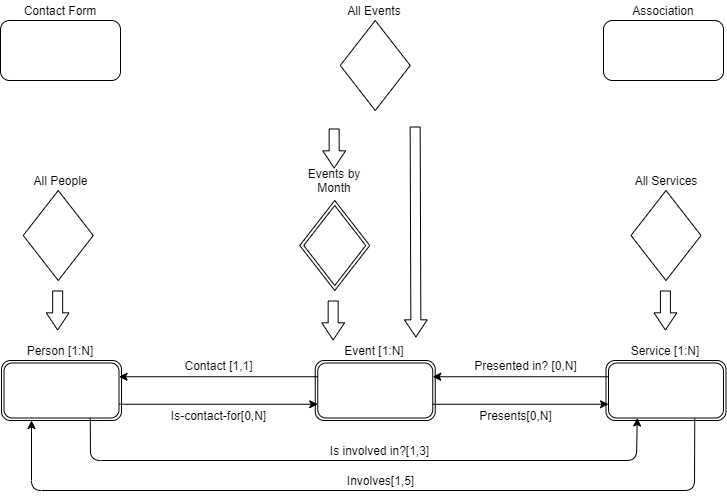
\includegraphics[width=\textwidth]{./assets/C-IDM.png}
			\caption{Content Interactive Dialogue Model}
		\end{minipage}
	\end{figure}
	\FloatBarrier

	\clearpage

	\subsection{L-IDM}
	\begin{figure}[h!]
		\centering
		\begin{minipage}[b]{1\textwidth}
    			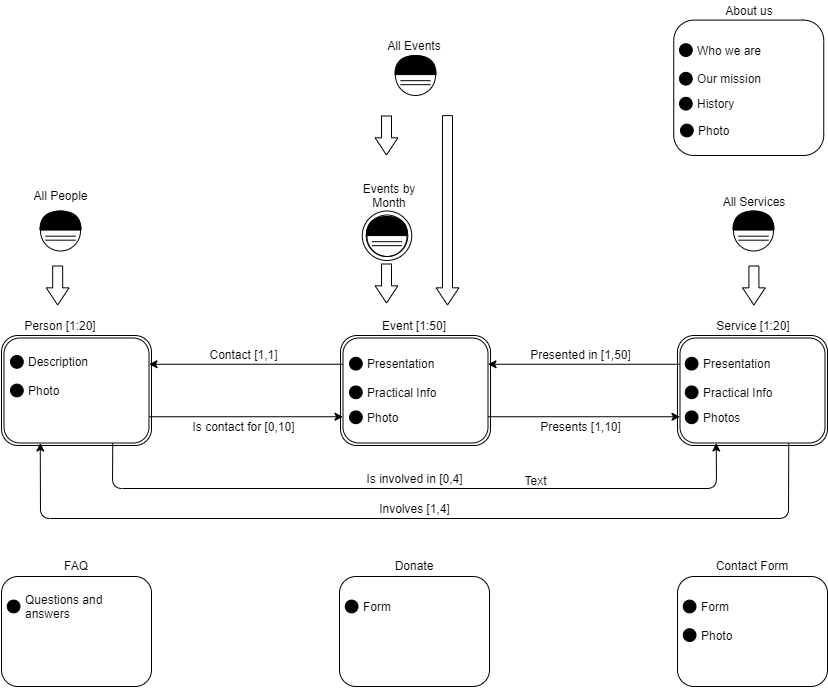
\includegraphics[width=\textwidth]{./assets/L-IDM.png}
			\caption{Logical Interactive Dialogue Model}
		\end{minipage}
	\end{figure}

	\clearpage

	\subsection{P-IDM}
	\begin{figure}[h!]
		\centering
		\begin{minipage}[b]{1\textwidth}
    			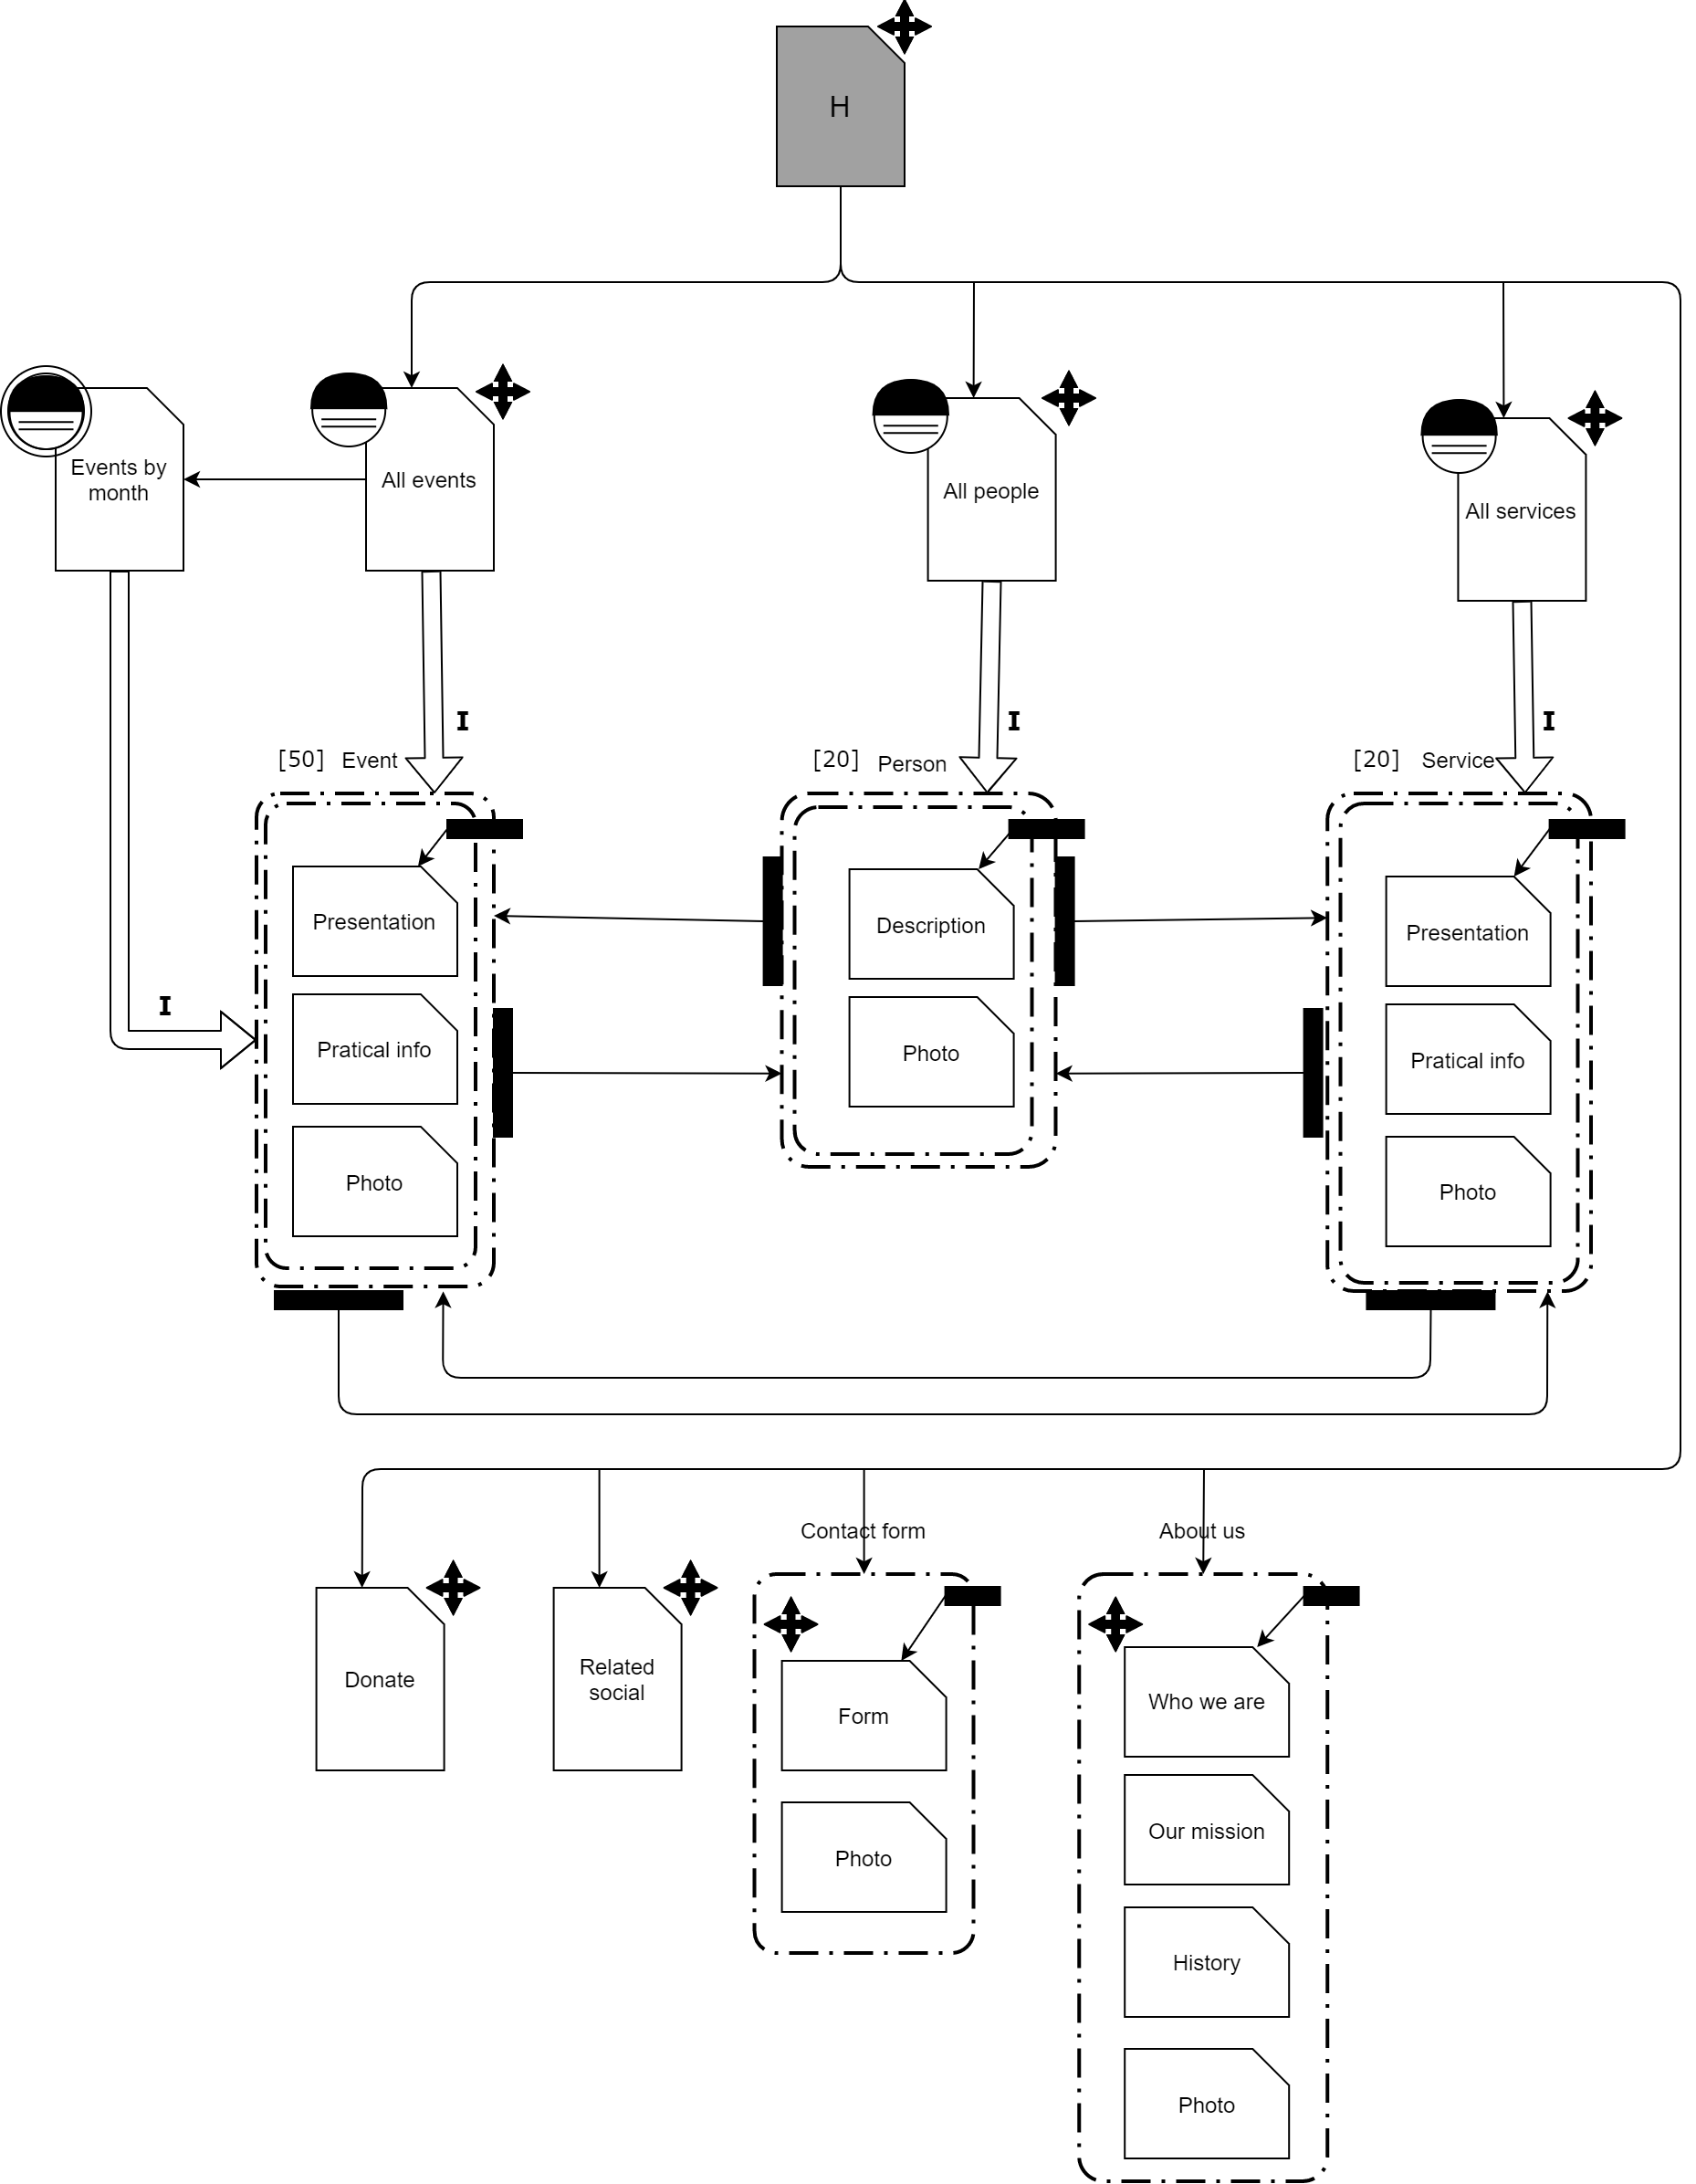
\includegraphics[width=\textwidth]{./assets/P-IDM.png}
			\caption{Page Interactive Dialogue Model}
		\end{minipage}
	\end{figure}
	\clearpage


	%Scenarios
	\section{Scenarios}

	\subsection{Case 1}
	An elementary school teacher that lives in Sondrio has always loved mountain fauna. One day she decides to bring her students in a trip to show them the beauty of those creatures, so she connects to the website.\\
First she learns some basics about the association, then she proceeds to search for an interesting event during the current month that presents several services involving different animals. When she finds the best event for what she is looking for, she contacts the volunteer responsible for that event to reserve a place for her class.
	\begin{figure}[h!]
		\centering
		\begin{minipage}[b]{1\textwidth}
    			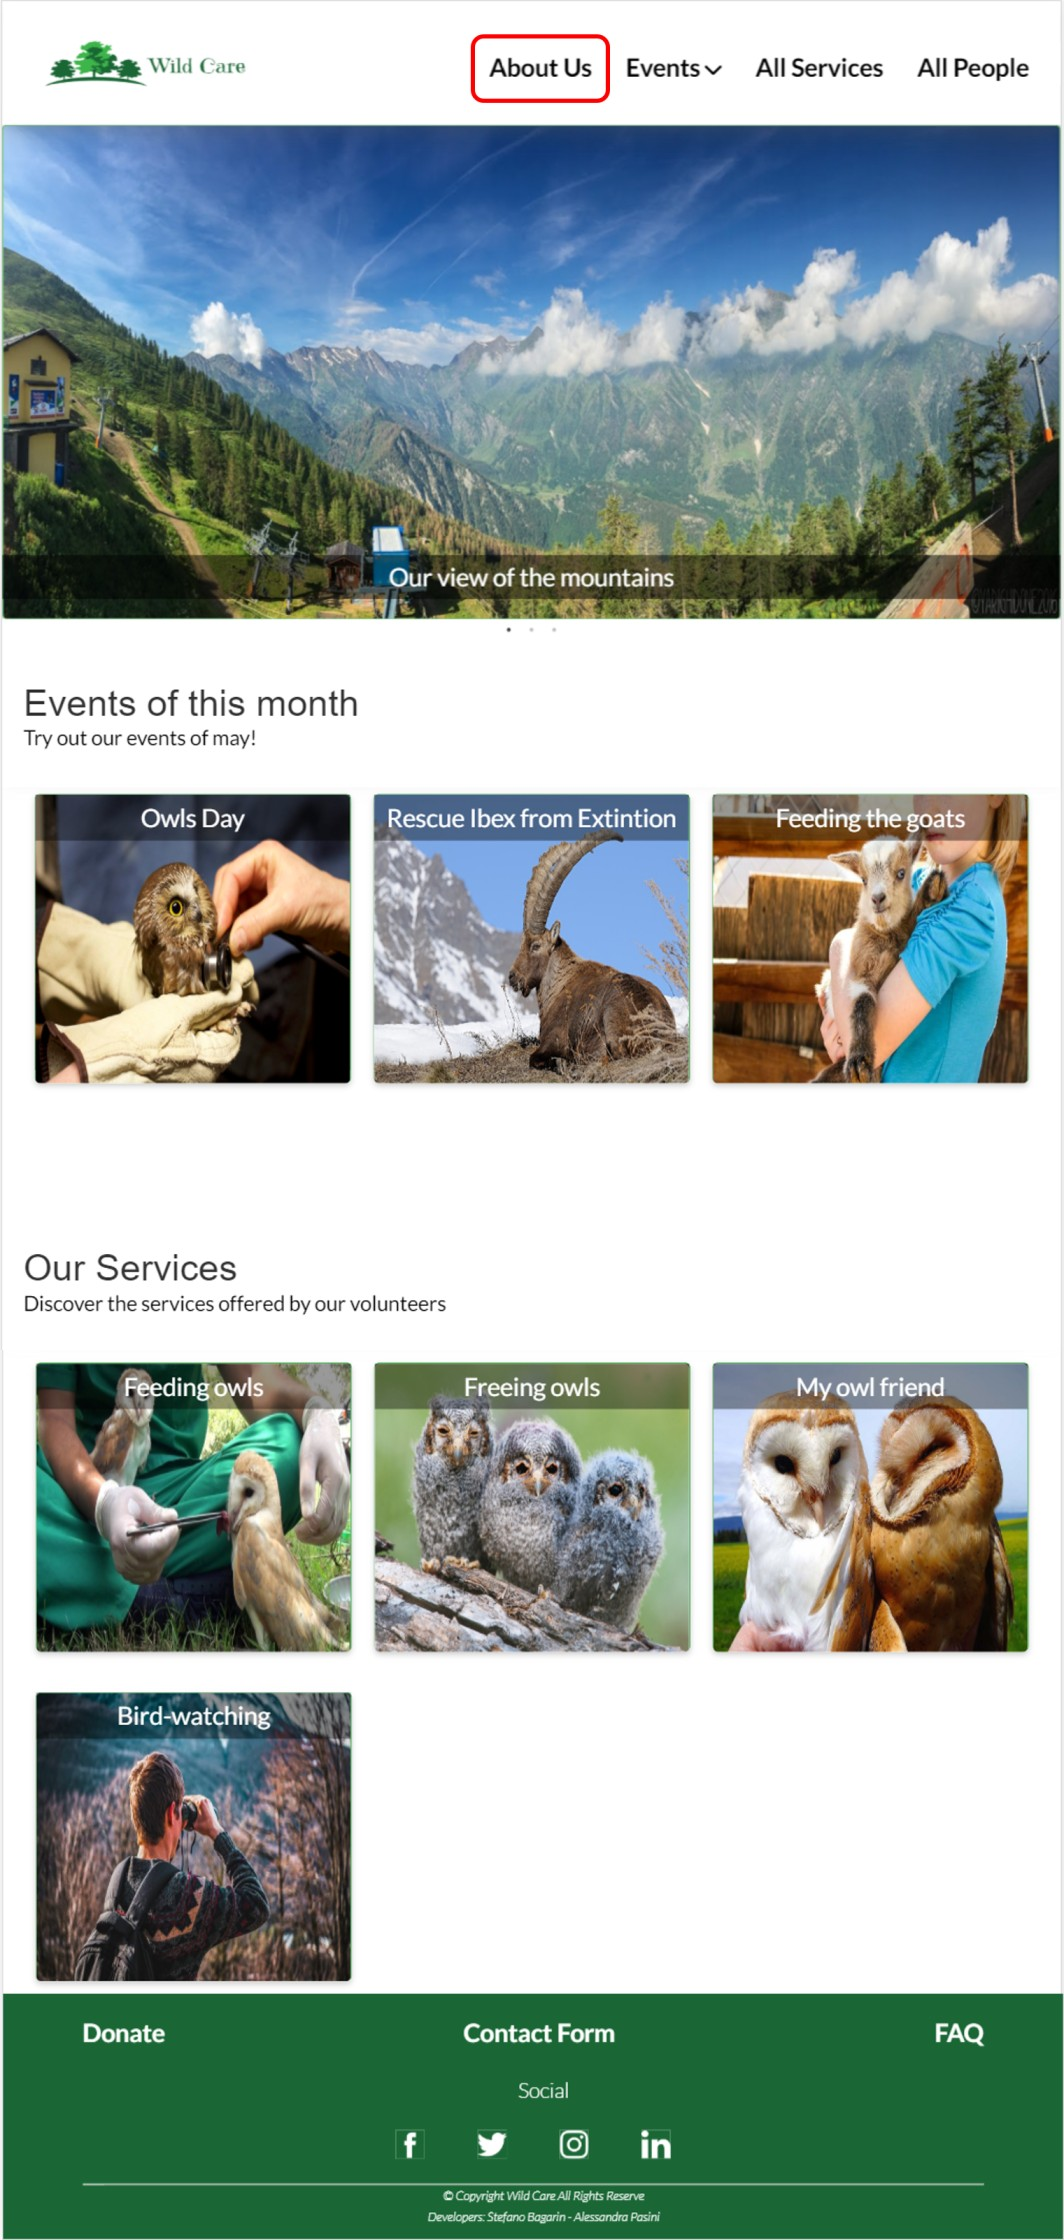
\includegraphics[width= 120mm]{./assets/mockups/homepage_aboutus.png}
			\caption{Selects about us from the home page.}
		\end{minipage}
	\end{figure}

	\begin{figure}[h!]
		\centering
		\begin{minipage}[b]{1\textwidth}
    			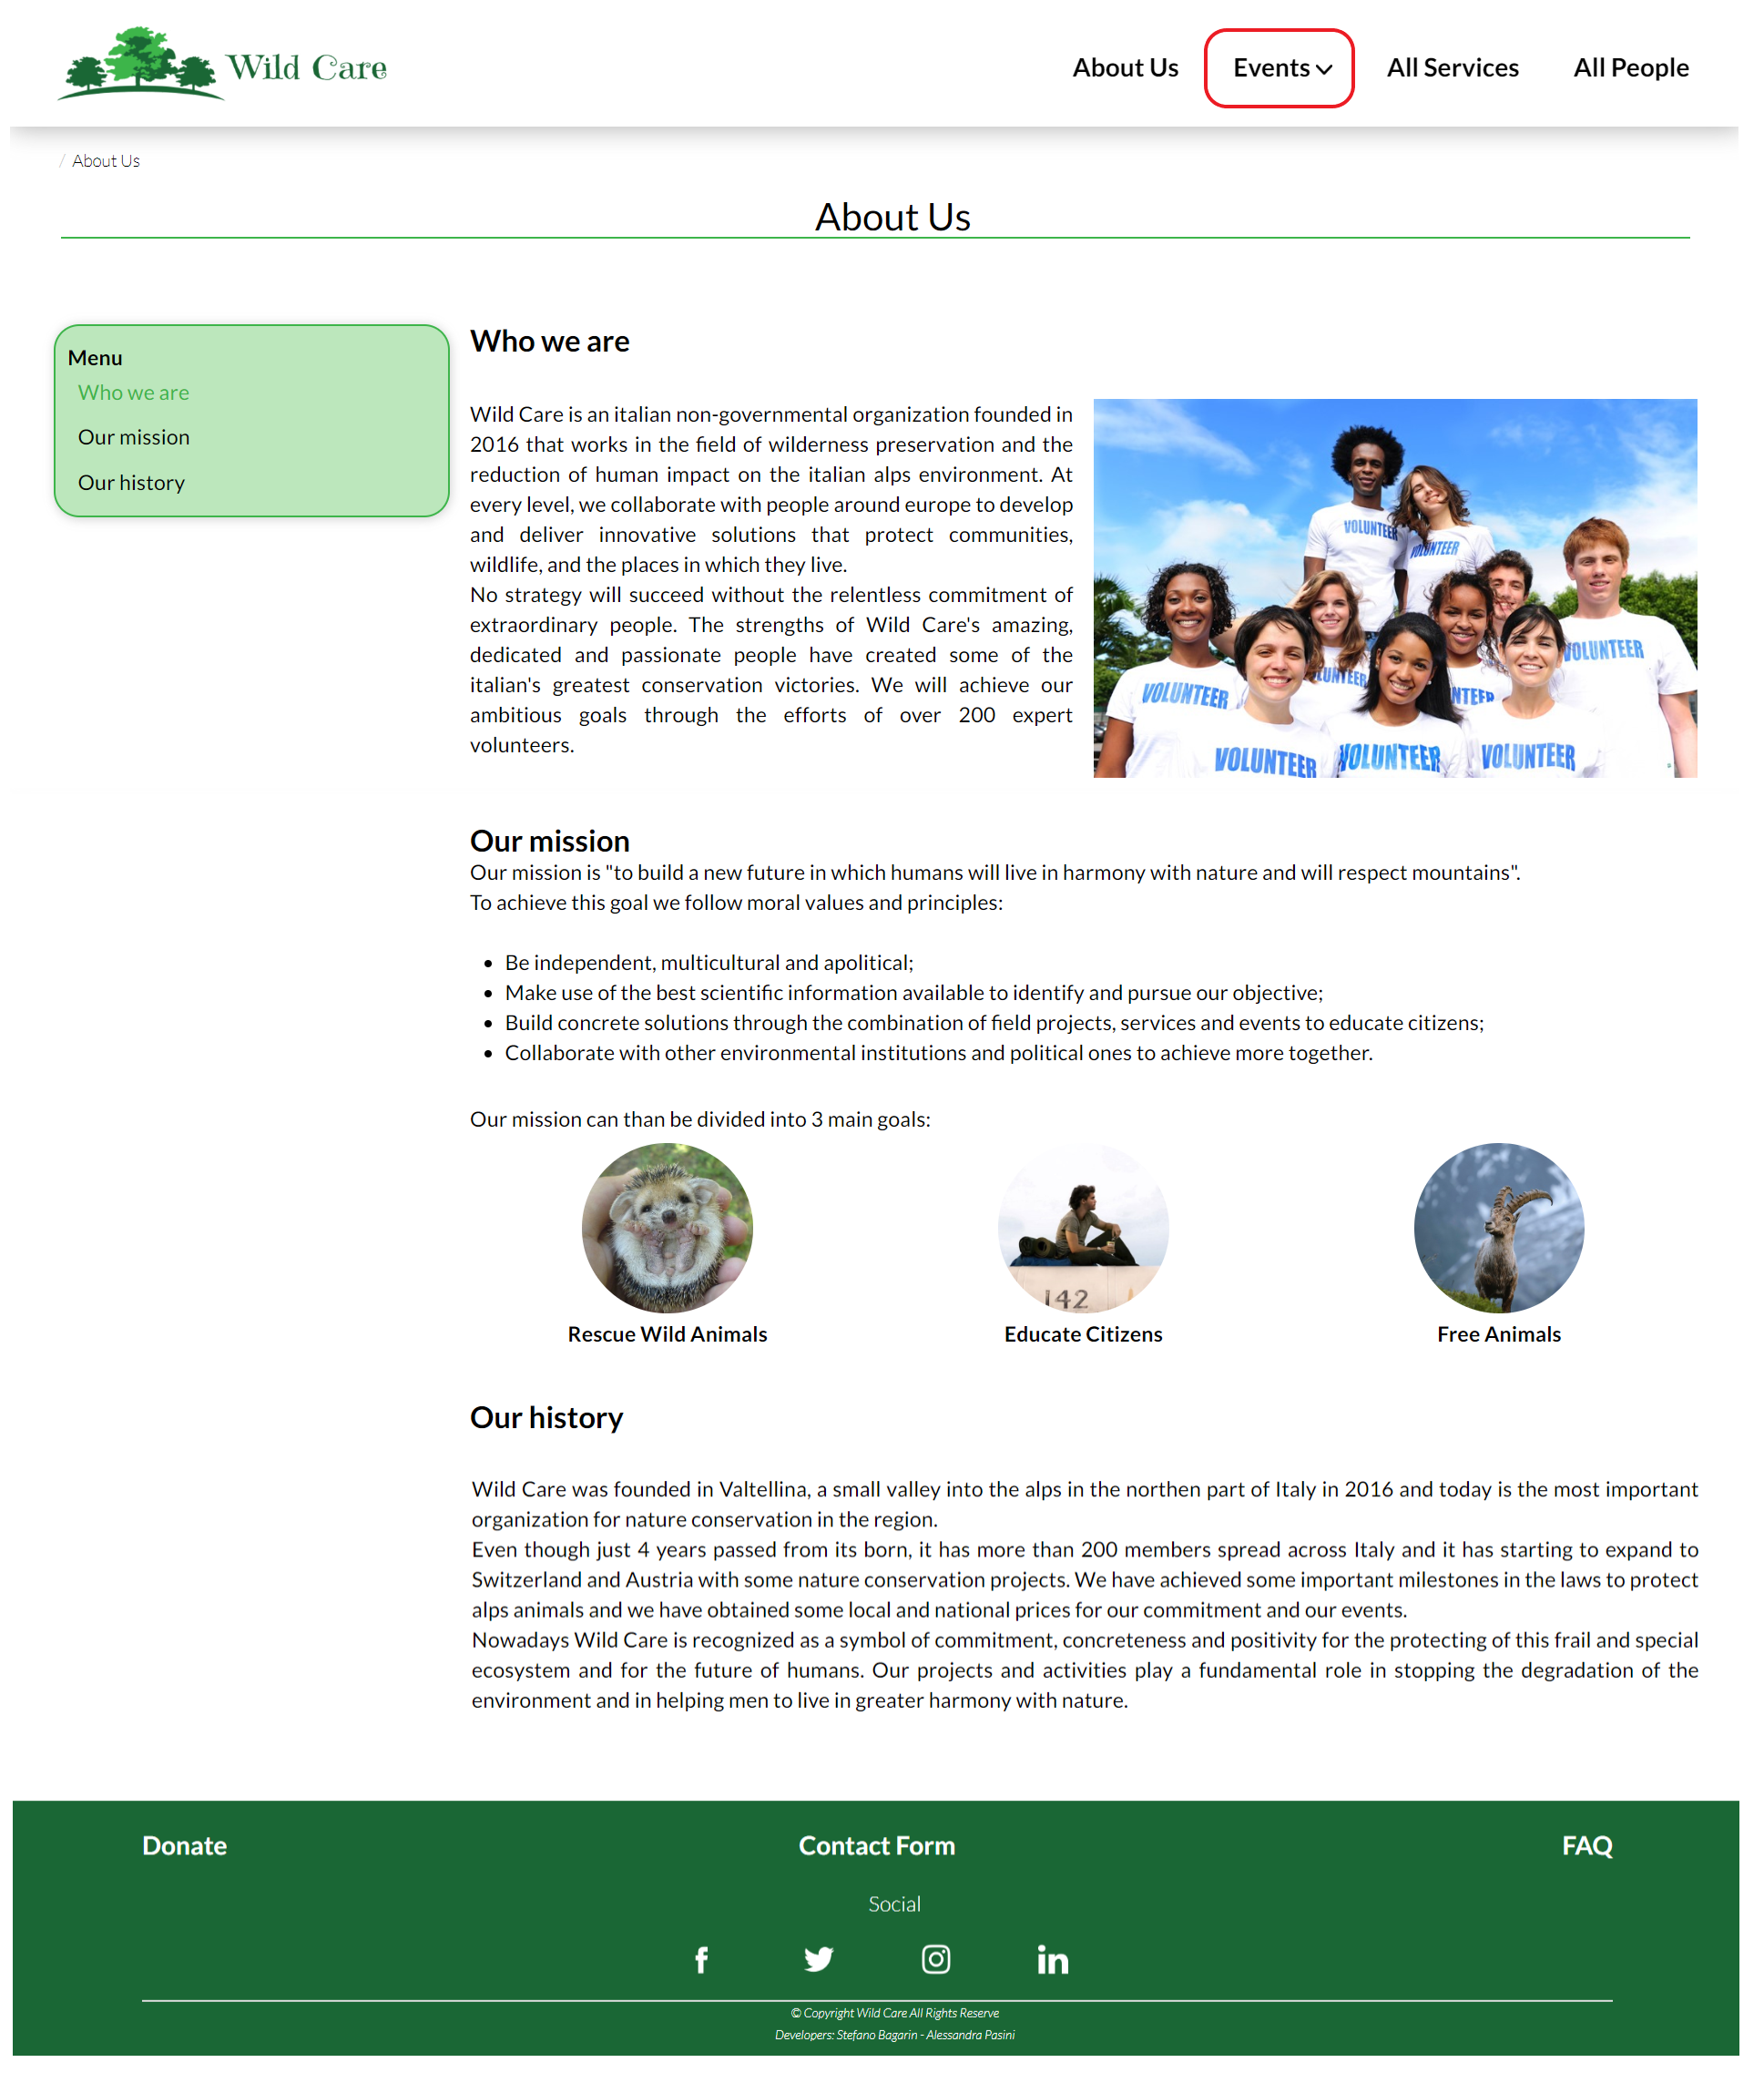
\includegraphics[width=\textwidth]{./assets/mockups/aboutus_eventsbymonth.png}
			\caption{Goes in the section events by month.}
		\end{minipage}
	\end{figure}

	\begin{figure}[h!]
		\centering
		\begin{minipage}[b]{1\textwidth}
    			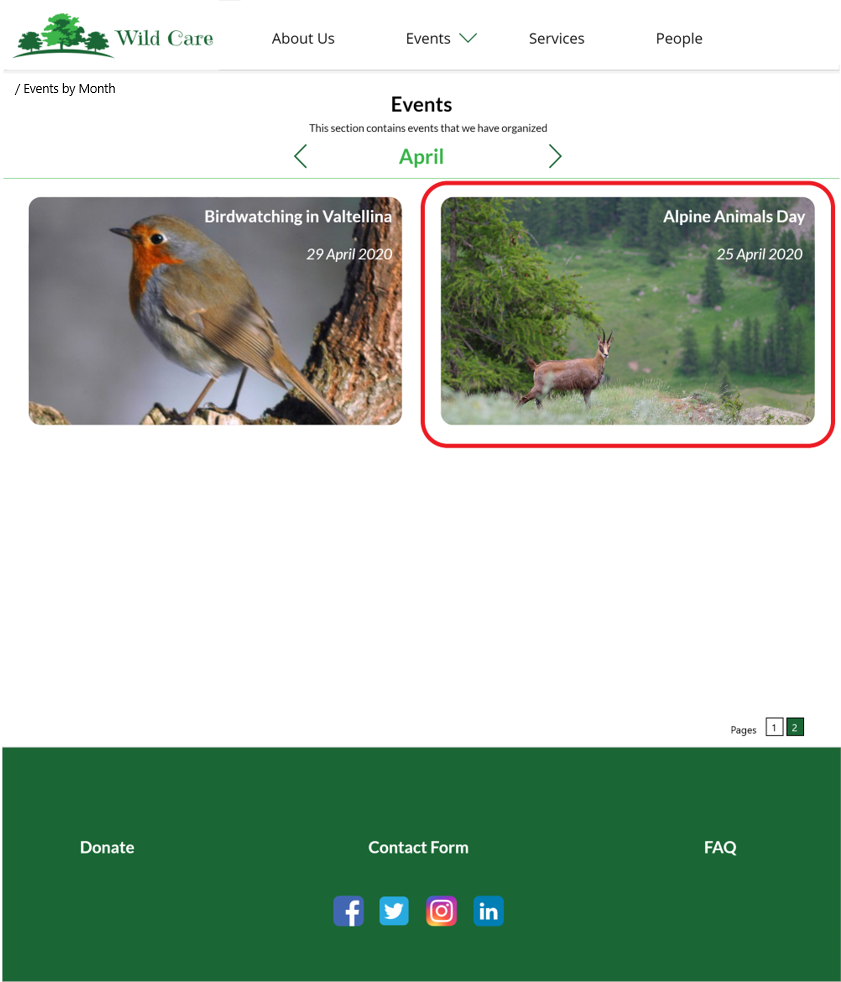
\includegraphics[width=\textwidth]{./assets/mockups/eventsbymonth_event.png}
			\caption{Selects an event.}
		\end{minipage}
	\end{figure}

	\begin{figure}[h!]
		\centering
		\begin{minipage}[b]{1\textwidth}
    			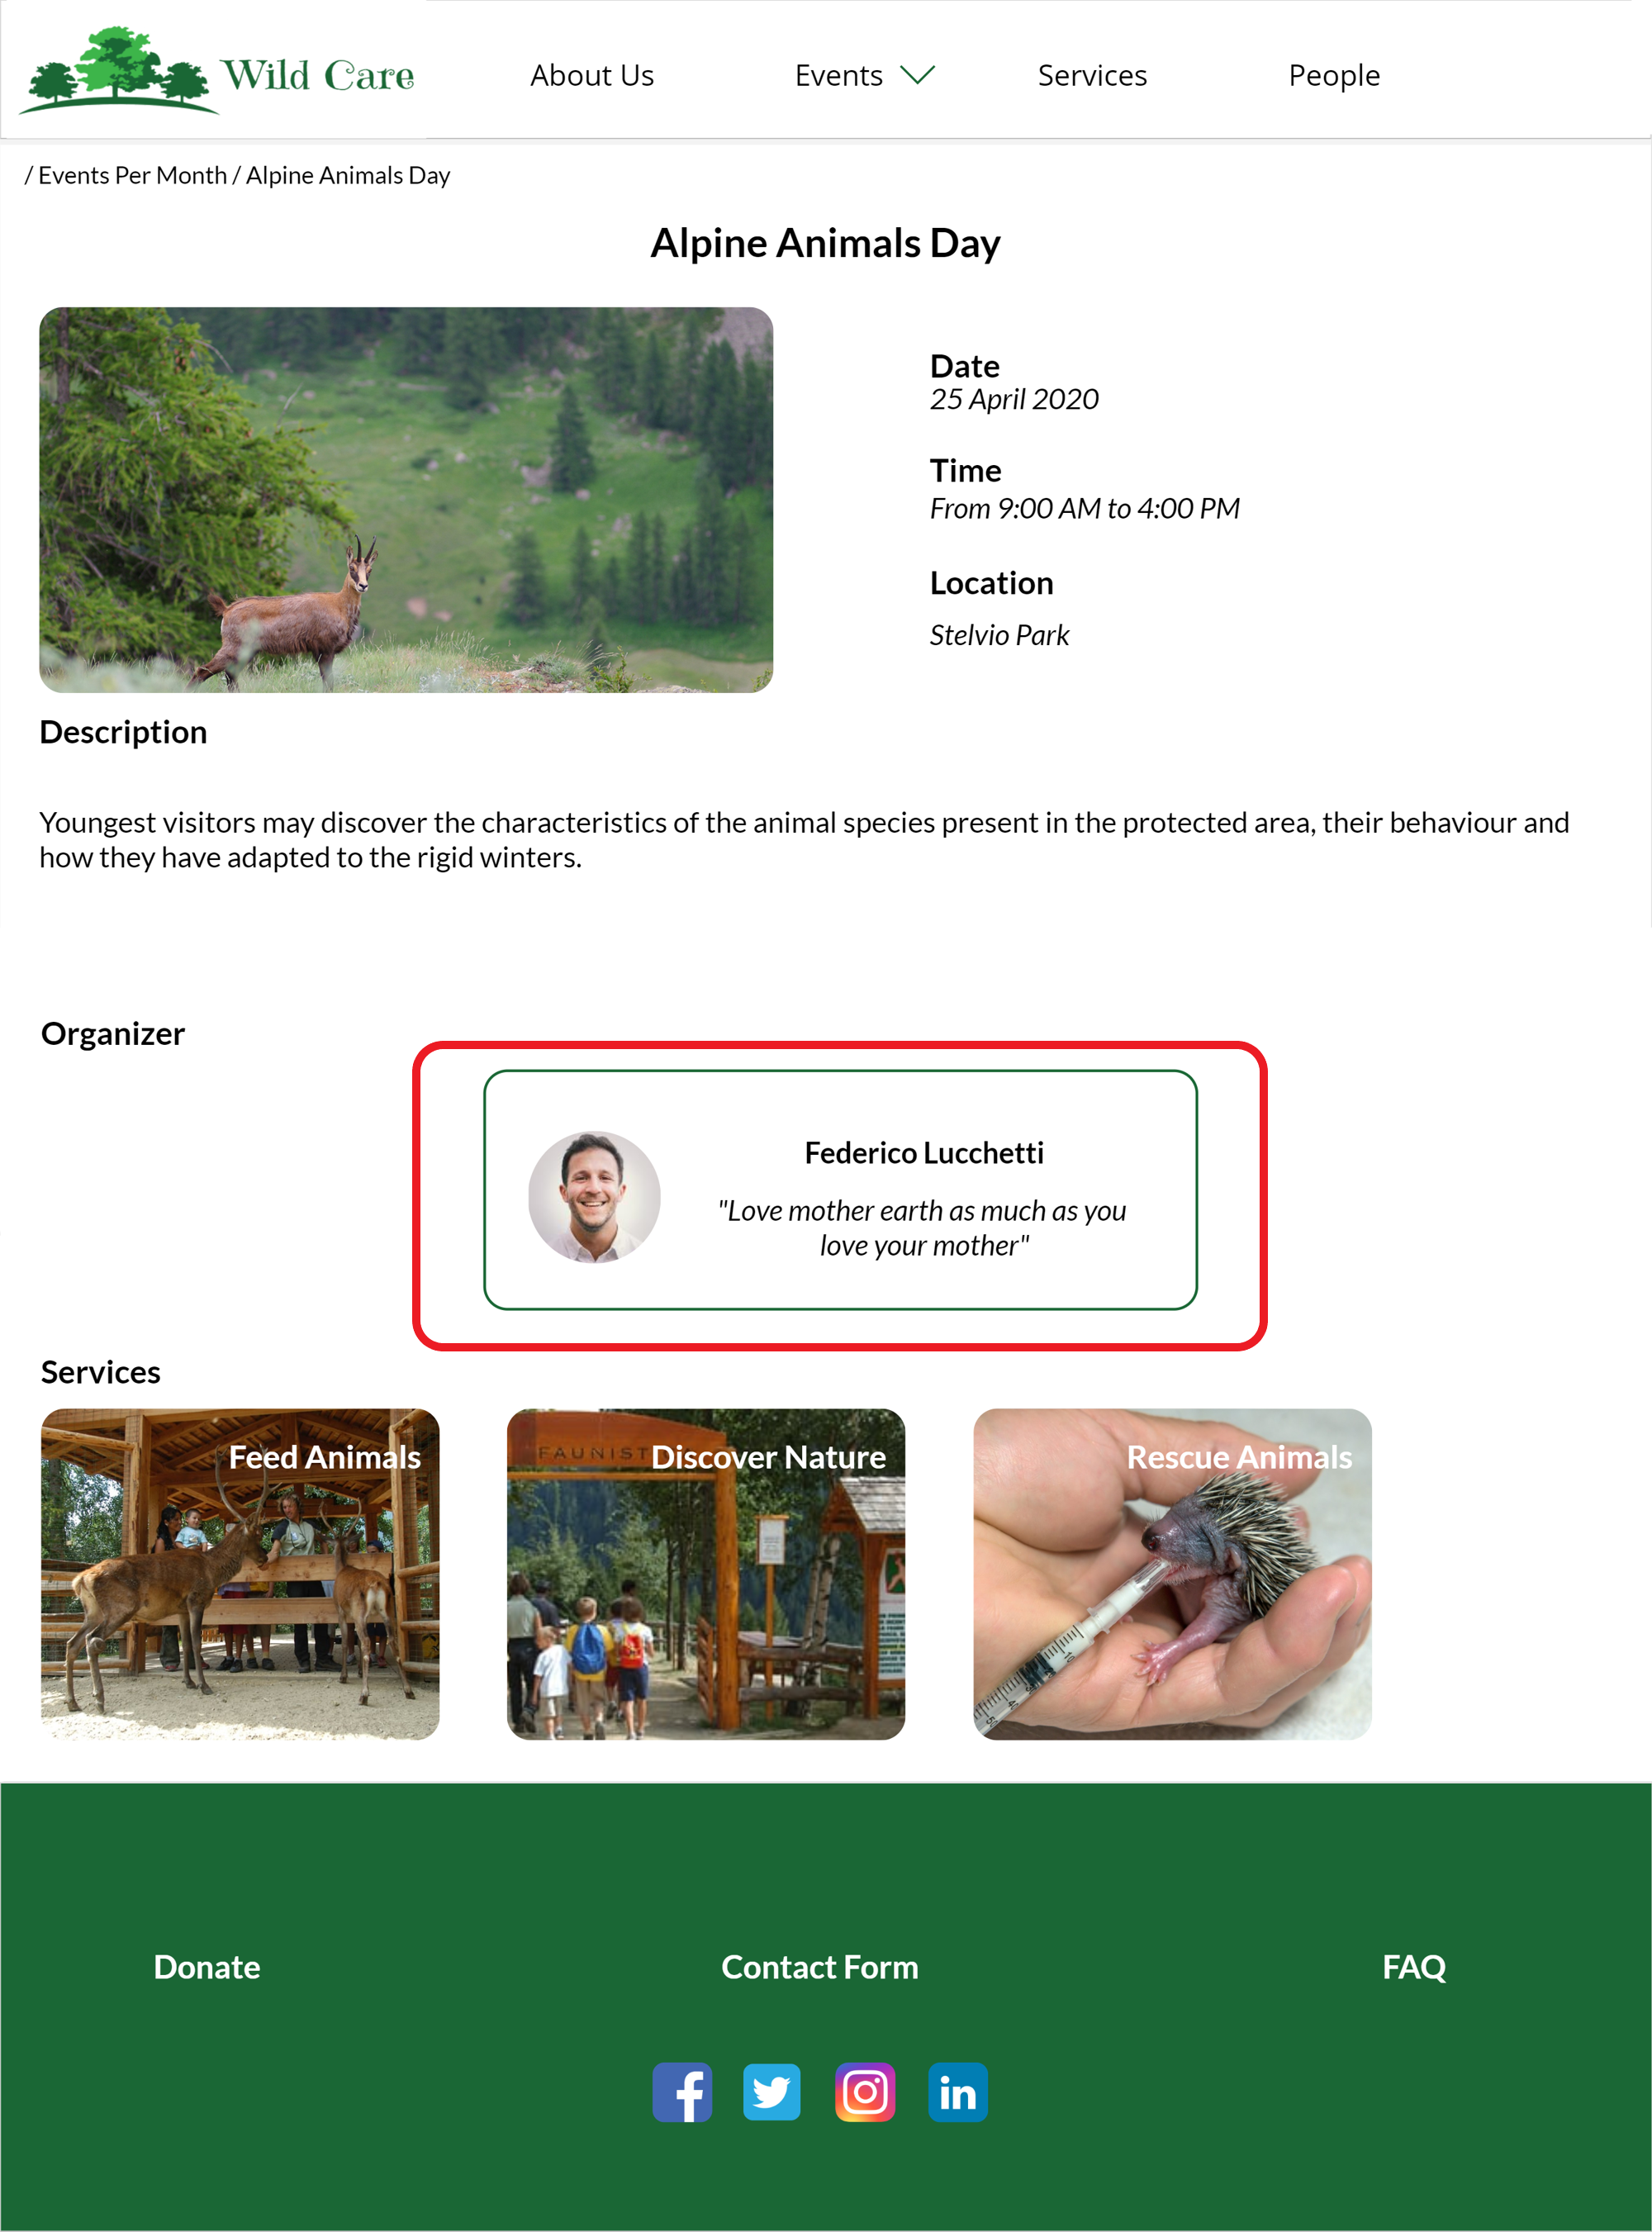
\includegraphics[width=\textwidth]{./assets/mockups/eventdetails_persondetails.png}
			\caption{Goes to the page of the responsible of the event.}
		\end{minipage}
	\end{figure}

	\begin{figure}[h!]
		\centering
		\begin{minipage}[b]{1\textwidth}
    			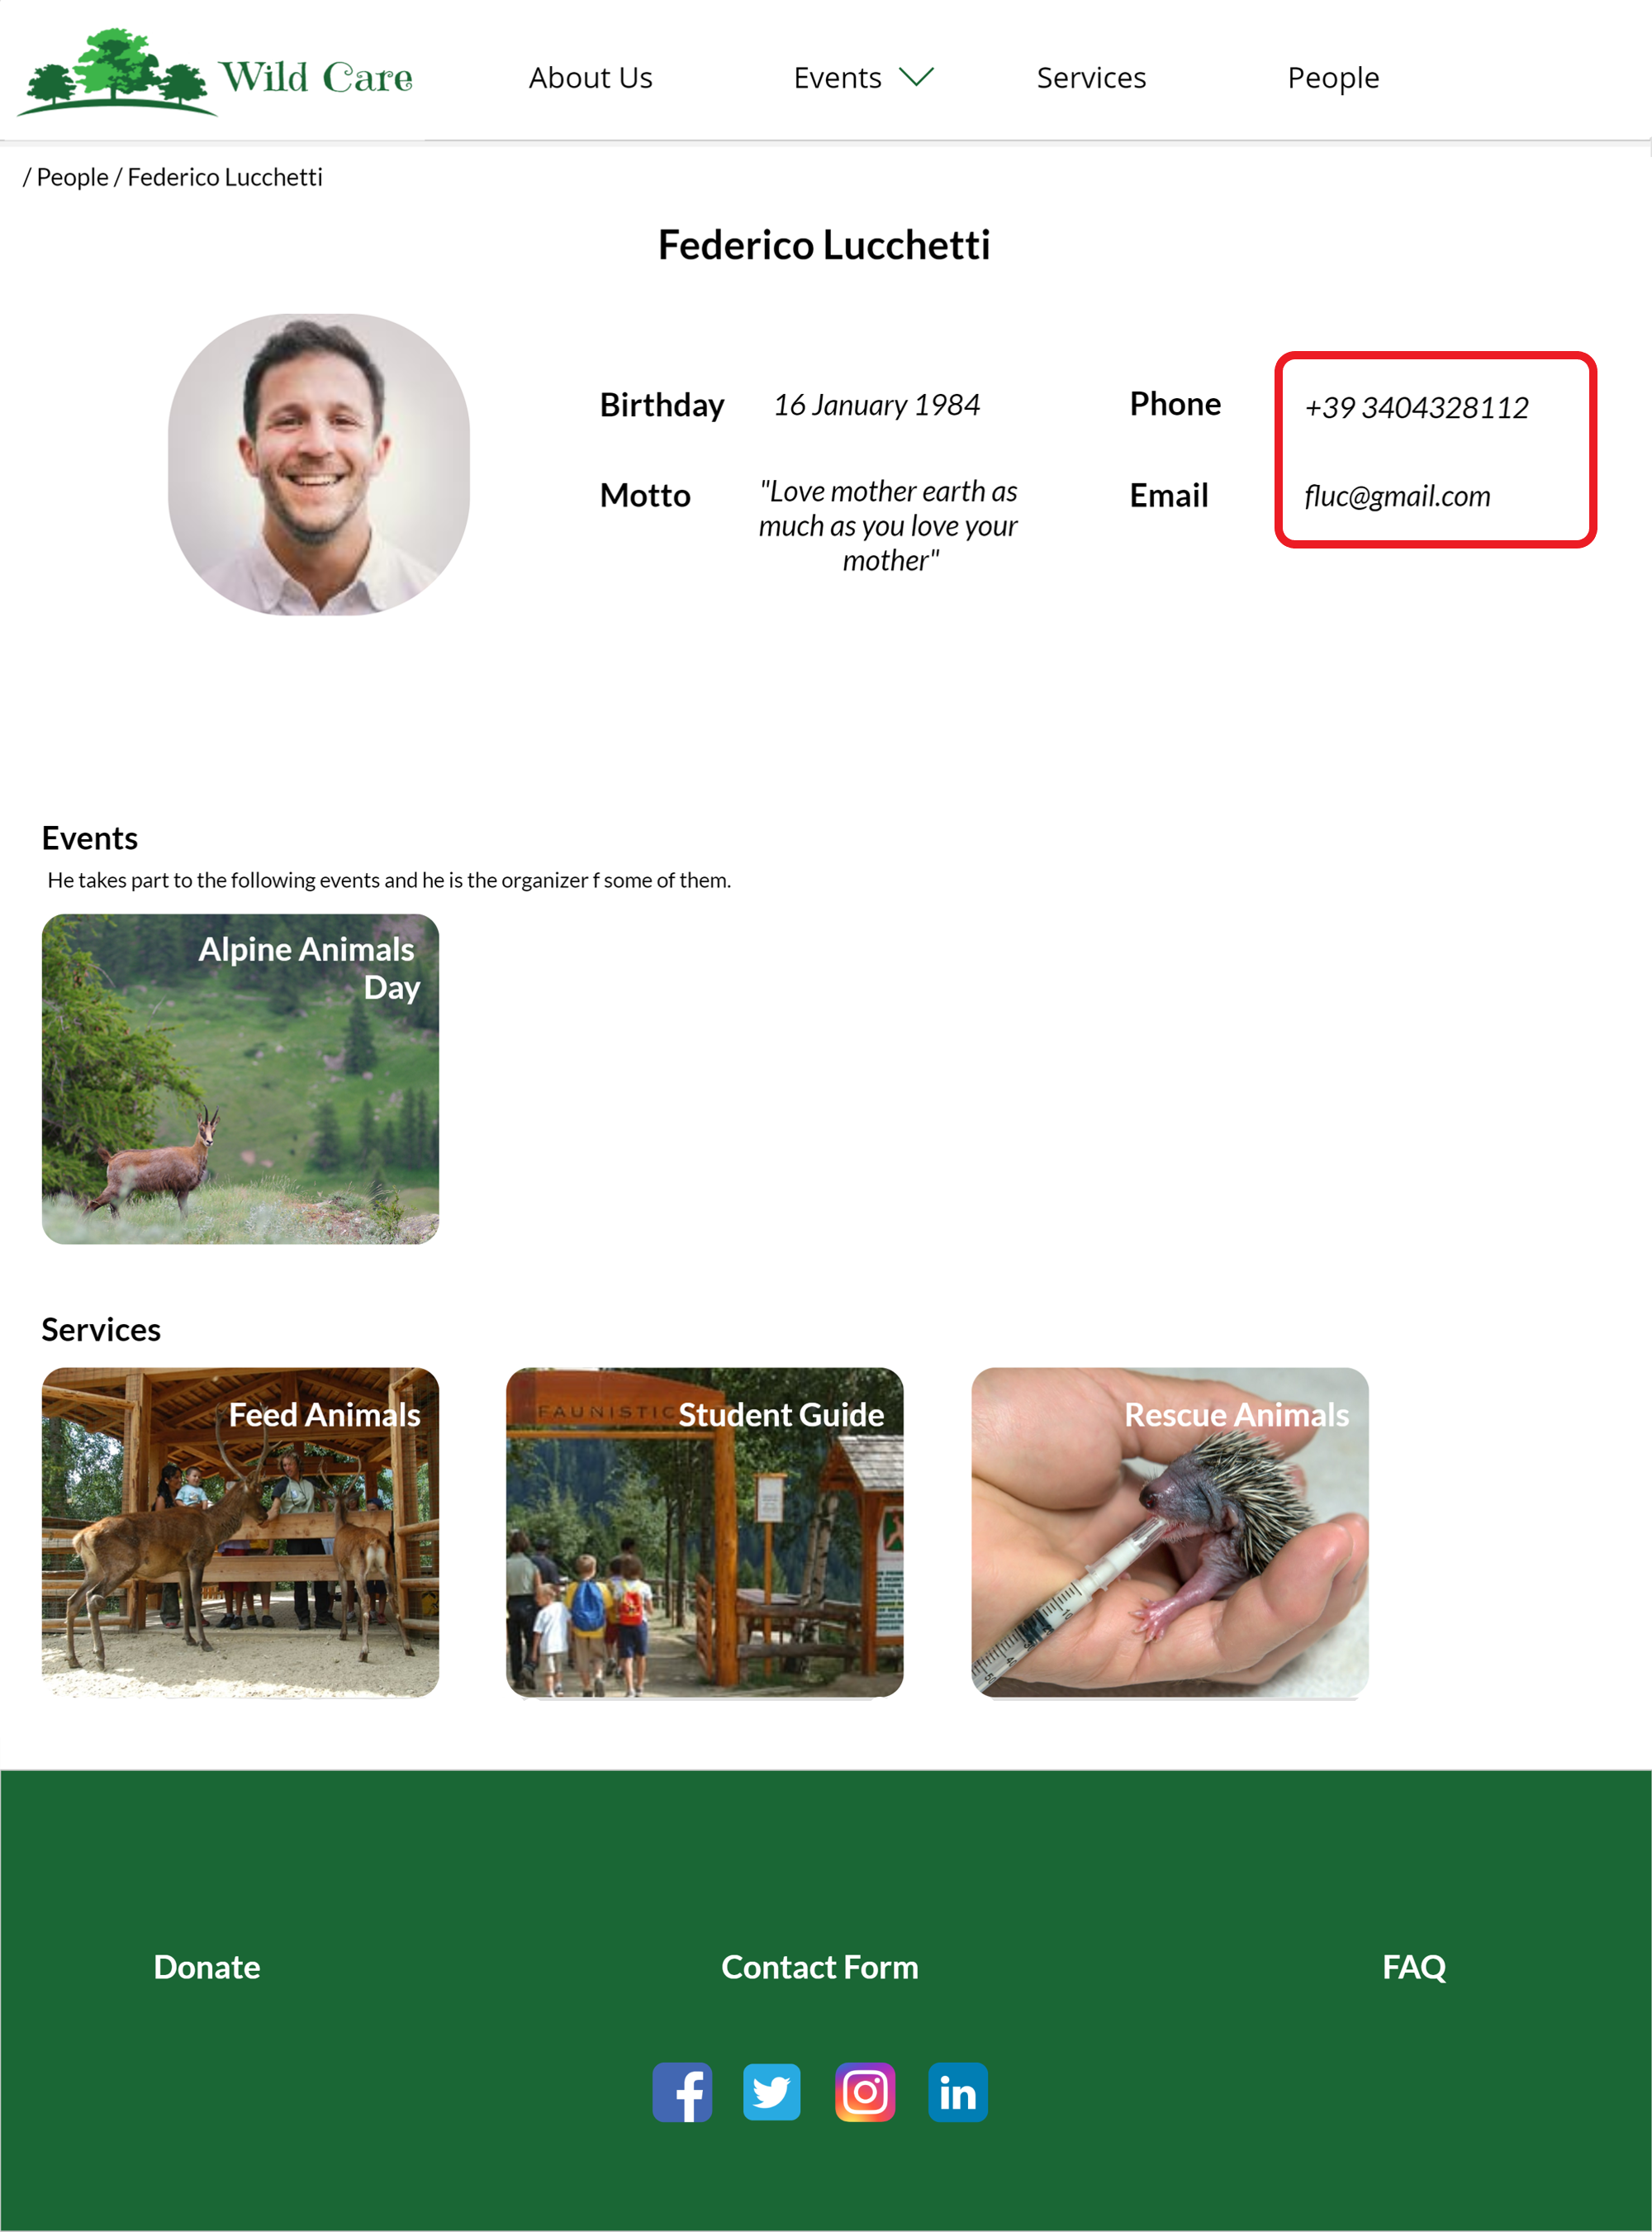
\includegraphics[width=\textwidth]{./assets/mockups/persondetails_contacts.png}
			\caption{Takes the email or the phone number of the responsible to contact it.}
		\end{minipage}
	\end{figure}
\clearpage

	\subsection{Case 2}
	Alessandra always watches documentaries abount mountain enviroment and she is scared about that fragile echosystem, so she decides to start to do something about it. She starts to looking for associations that takes care of wild animals and ends up on the website. \\
She reads all the informations about Wild Care and the profiles of some of the people that are already volunteers there and at the end decides that she likes the place; so she navigates to the FAQ section where she learns that to become a volunteer she needs to send a message to the association through the contact form.

	\begin{figure}[h!]
		\centering
		\begin{minipage}[b]{1\textwidth}
    			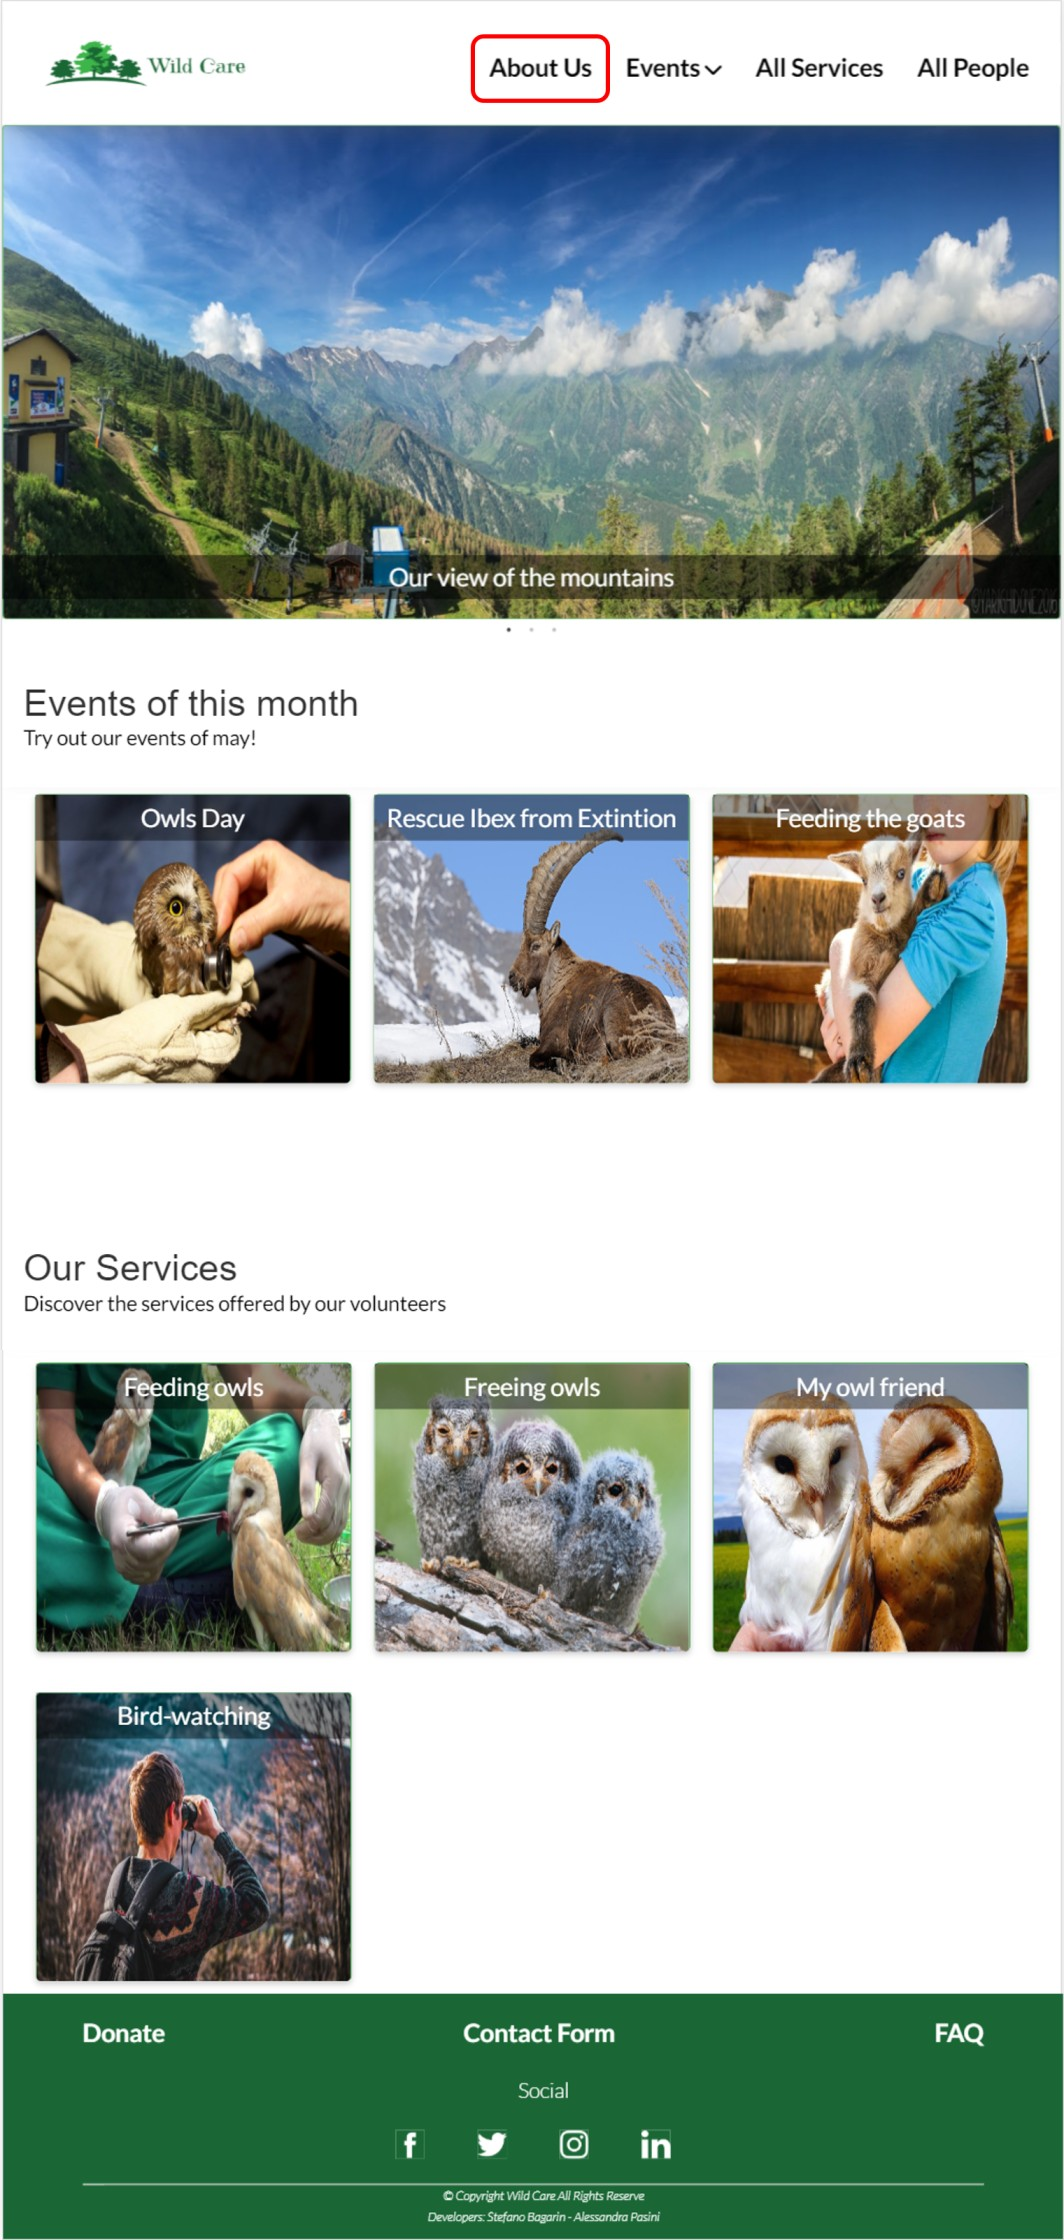
\includegraphics[width= 120mm]{./assets/mockups/homepage_aboutus.png}
			\caption{Selects about us from the home page.}
		\end{minipage}
	\end{figure}

	\begin{figure}[h!]
		\centering
		\begin{minipage}[b]{1\textwidth}
    			\includegraphics[width=\textwidth]{./assets/mockups/homepage.png}
			\caption{Goes in the people section.}
		\end{minipage}
	\end{figure}

	\begin{figure}[h!]
		\centering
		\begin{minipage}[b]{1\textwidth}
    			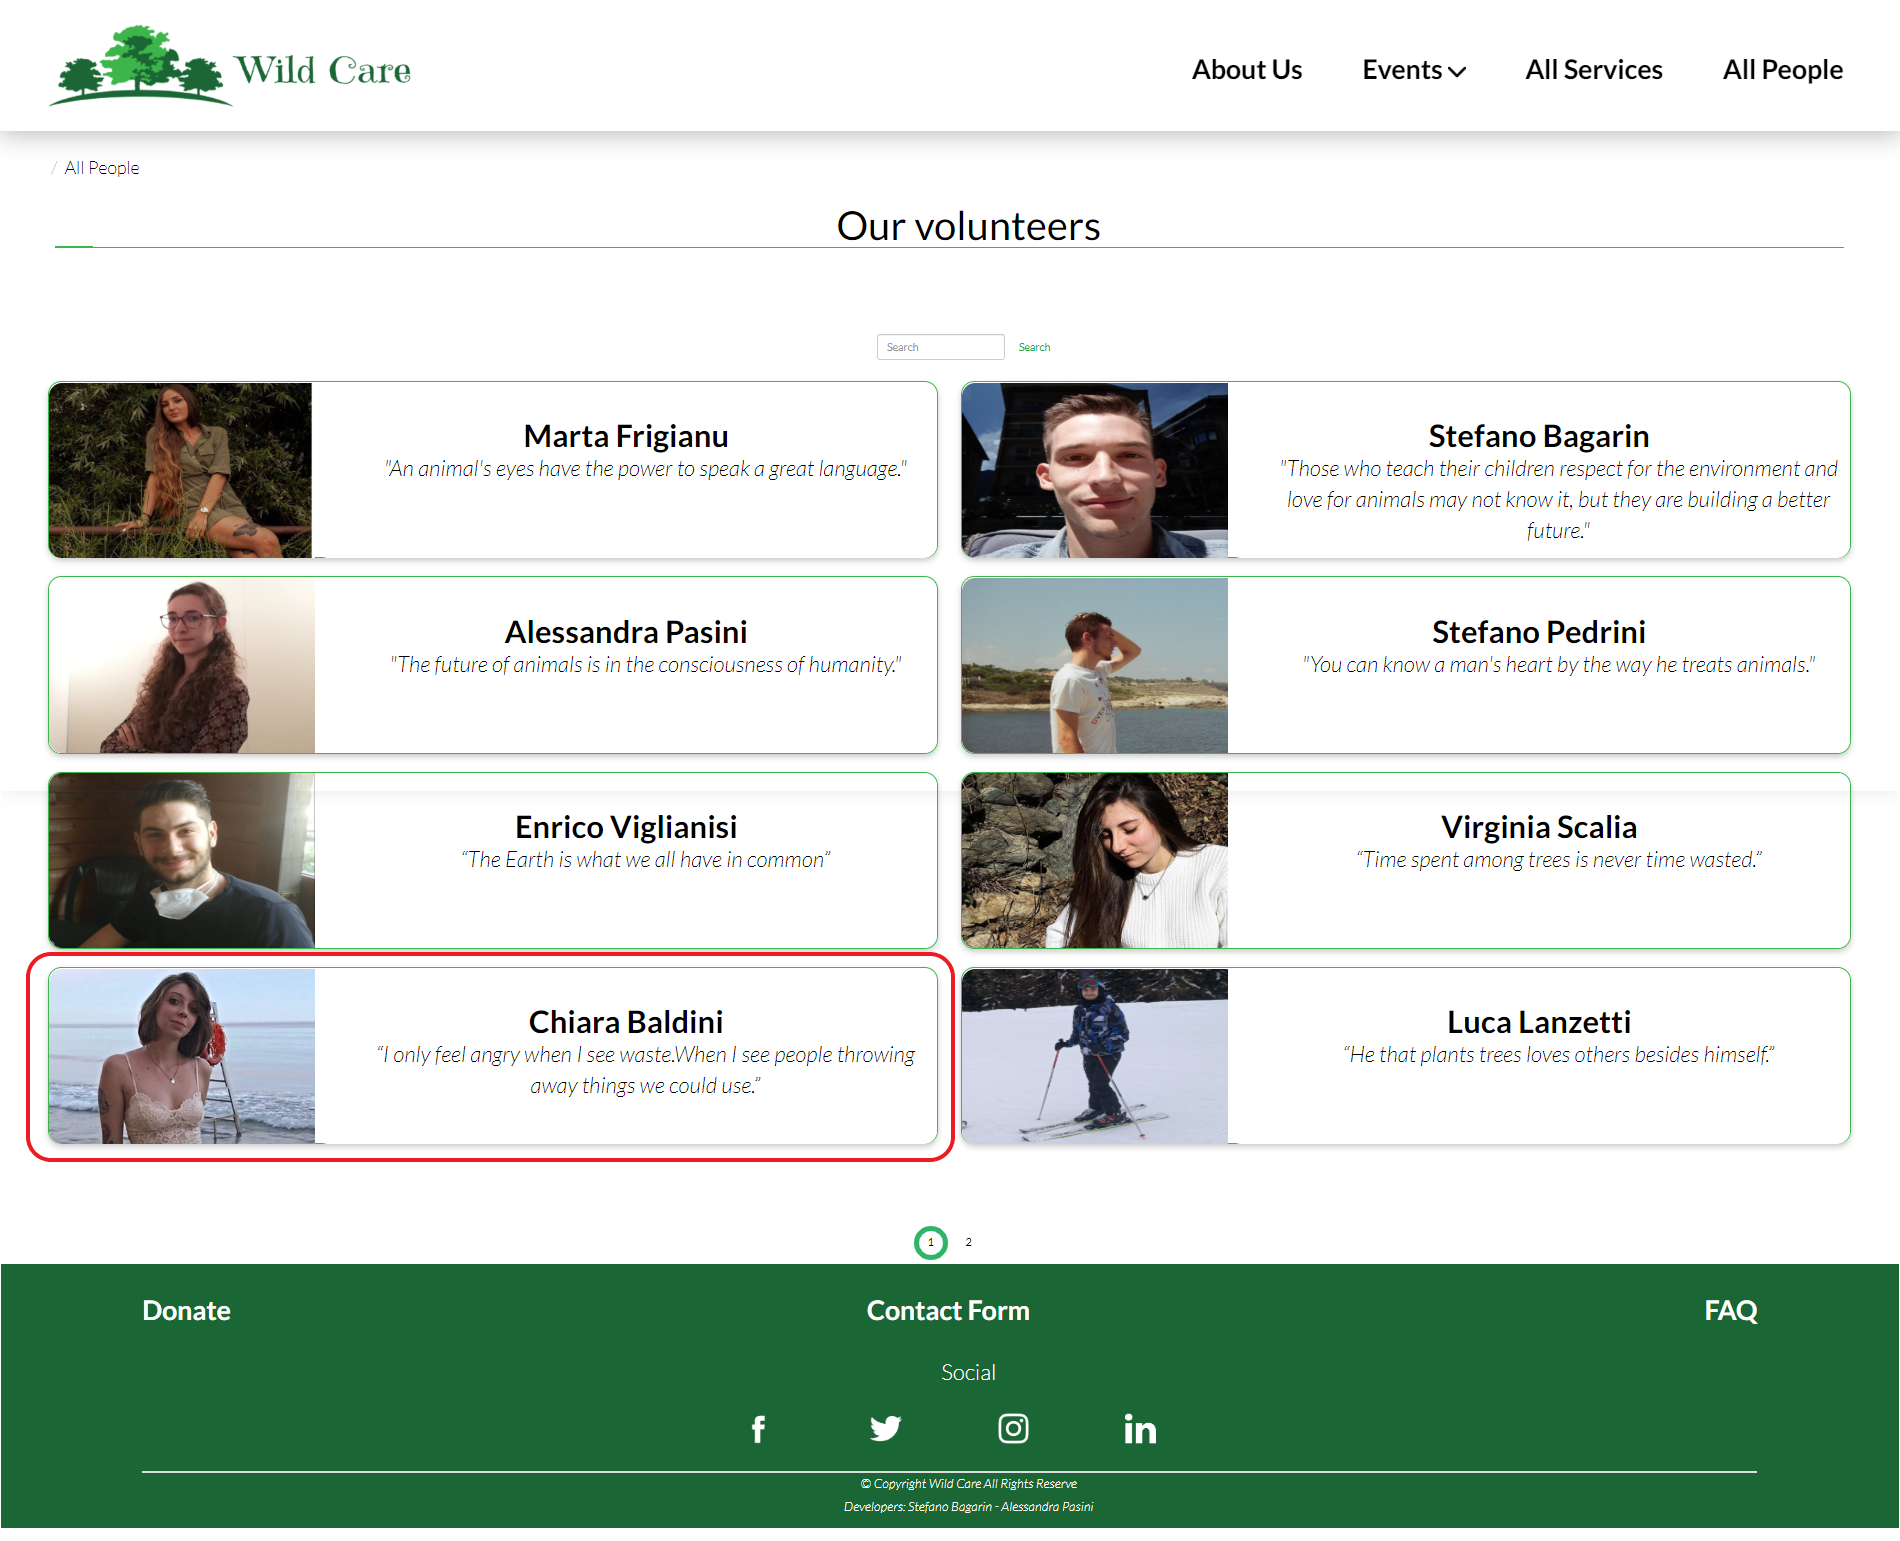
\includegraphics[width=\textwidth]{./assets/mockups/people_persondetails.png}
			\caption{Selects a person.}
		\end{minipage}
	\end{figure}

	\begin{figure}[h!]
		\centering
		\begin{minipage}[b]{1\textwidth}
    			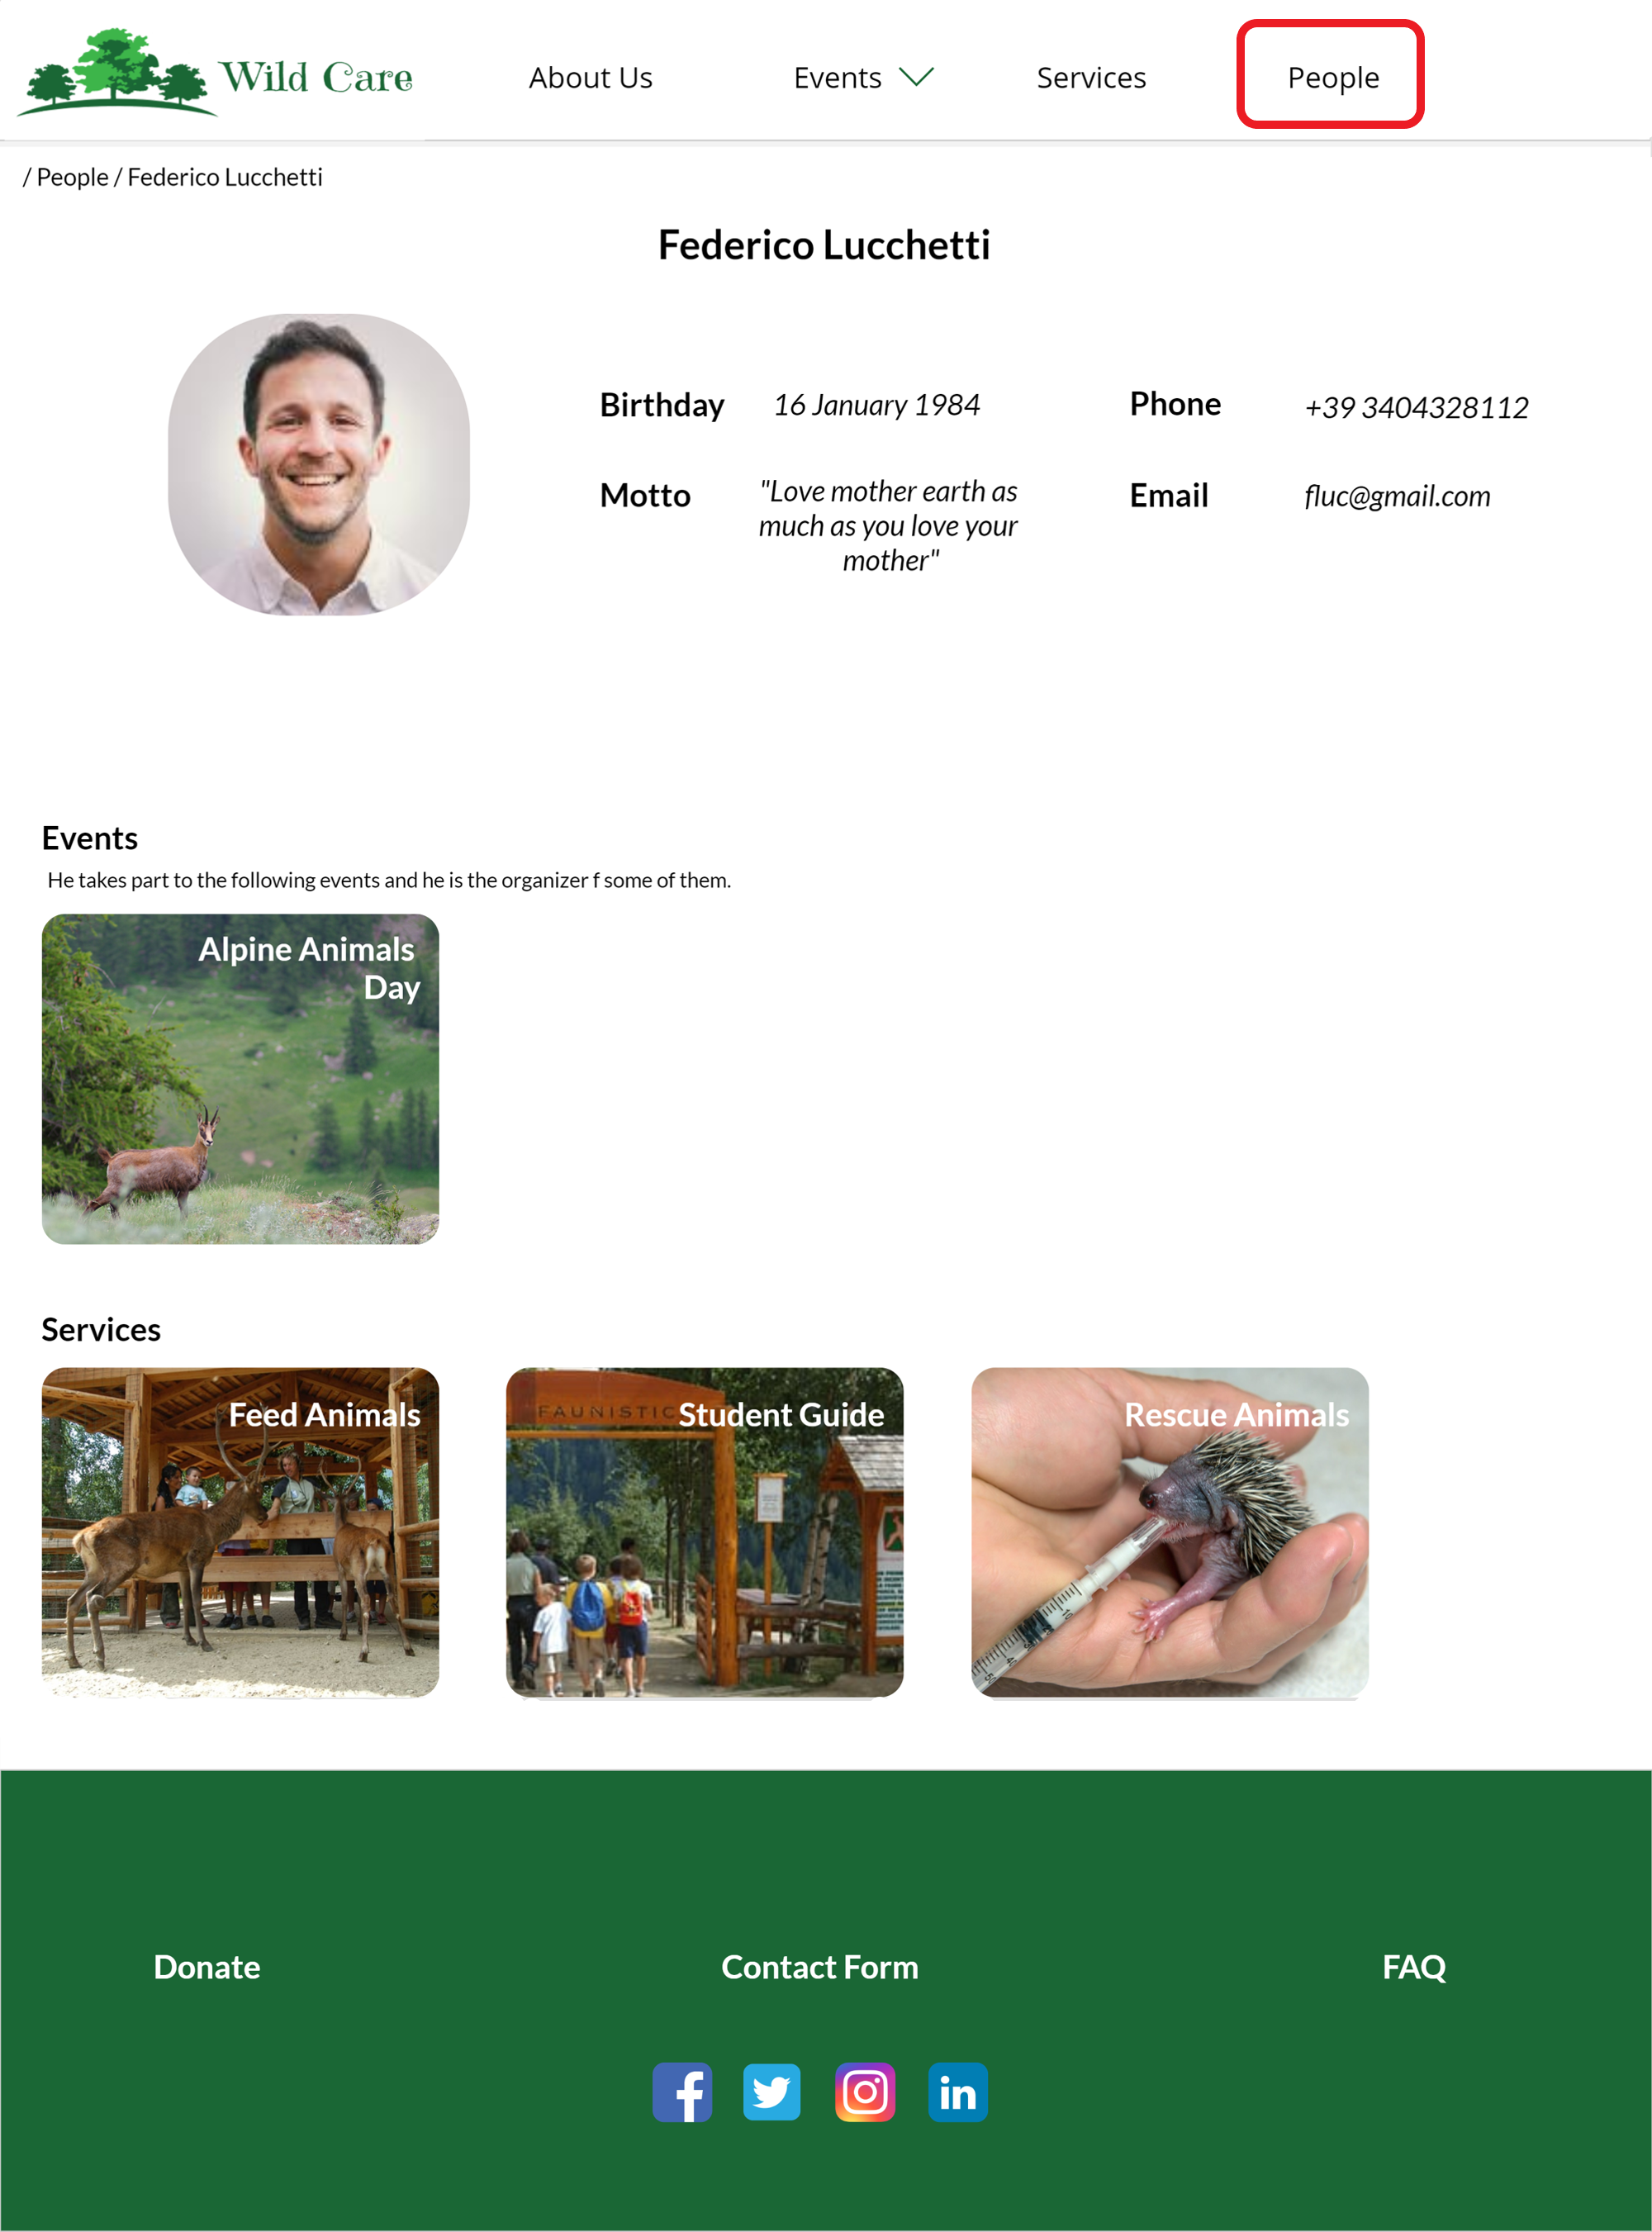
\includegraphics[width=\textwidth]{./assets/mockups/persondetails_people.png}
			\caption{Goes back to the people page to see the profile of other volunteers.}
		\end{minipage}
	\end{figure}

	\begin{figure}[h!]
		\centering
		\begin{minipage}[b]{1\textwidth}
    			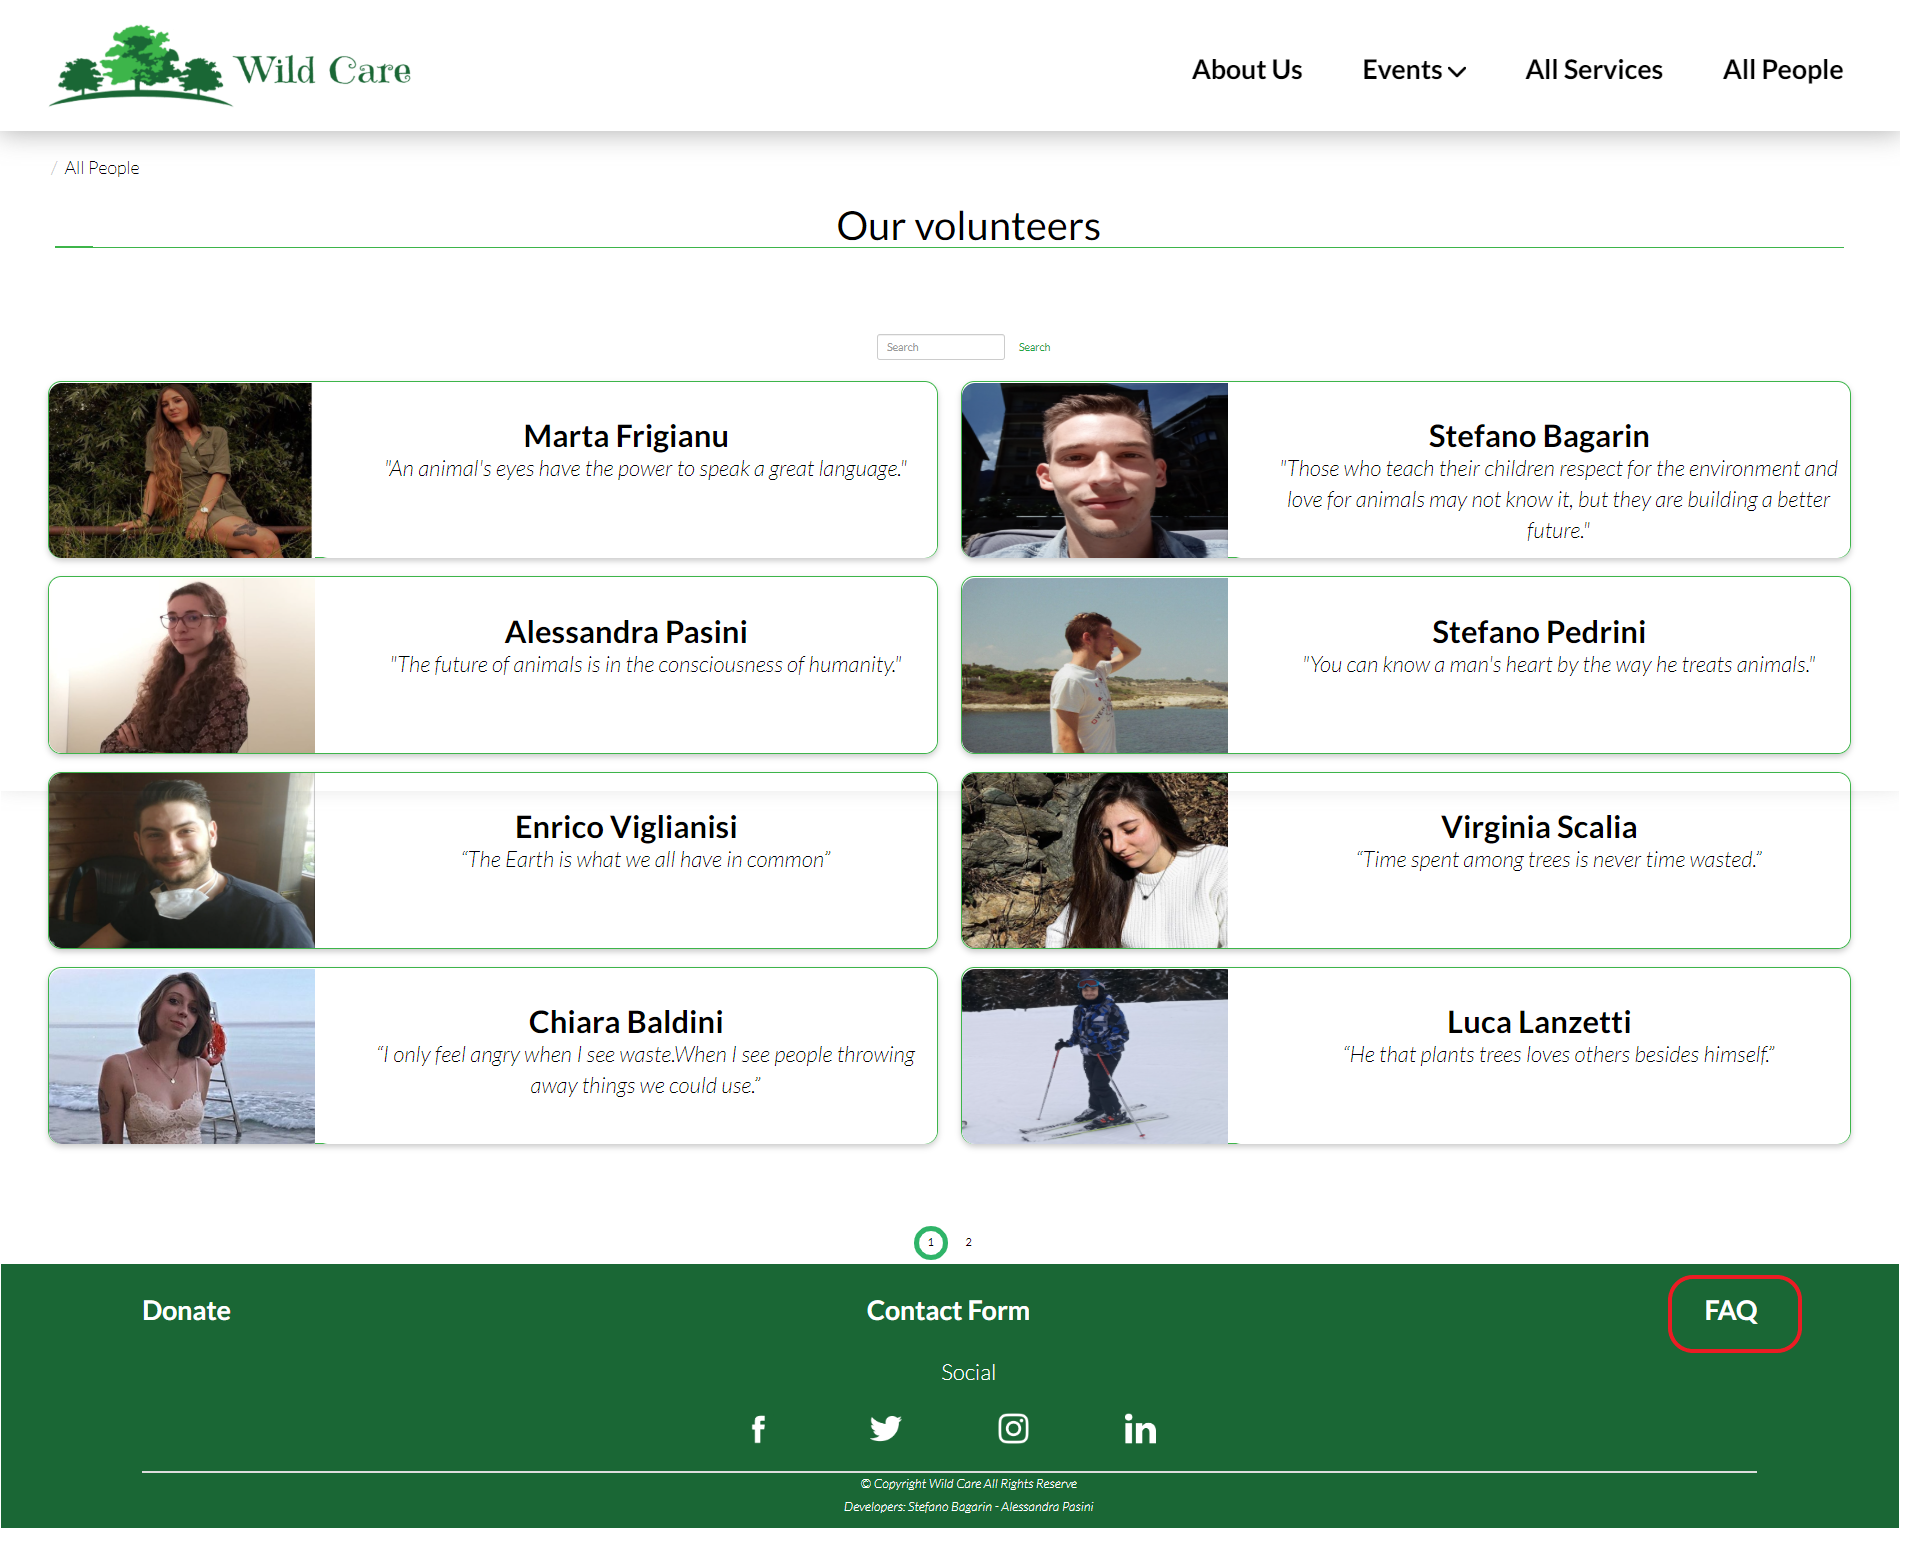
\includegraphics[width=\textwidth]{./assets/mockups/people_faq.png}
			\caption{Navigates to the FAQ section.}
		\end{minipage}
	\end{figure}

	\begin{figure}[h!]
		\centering
		\begin{minipage}[b]{1\textwidth}
    			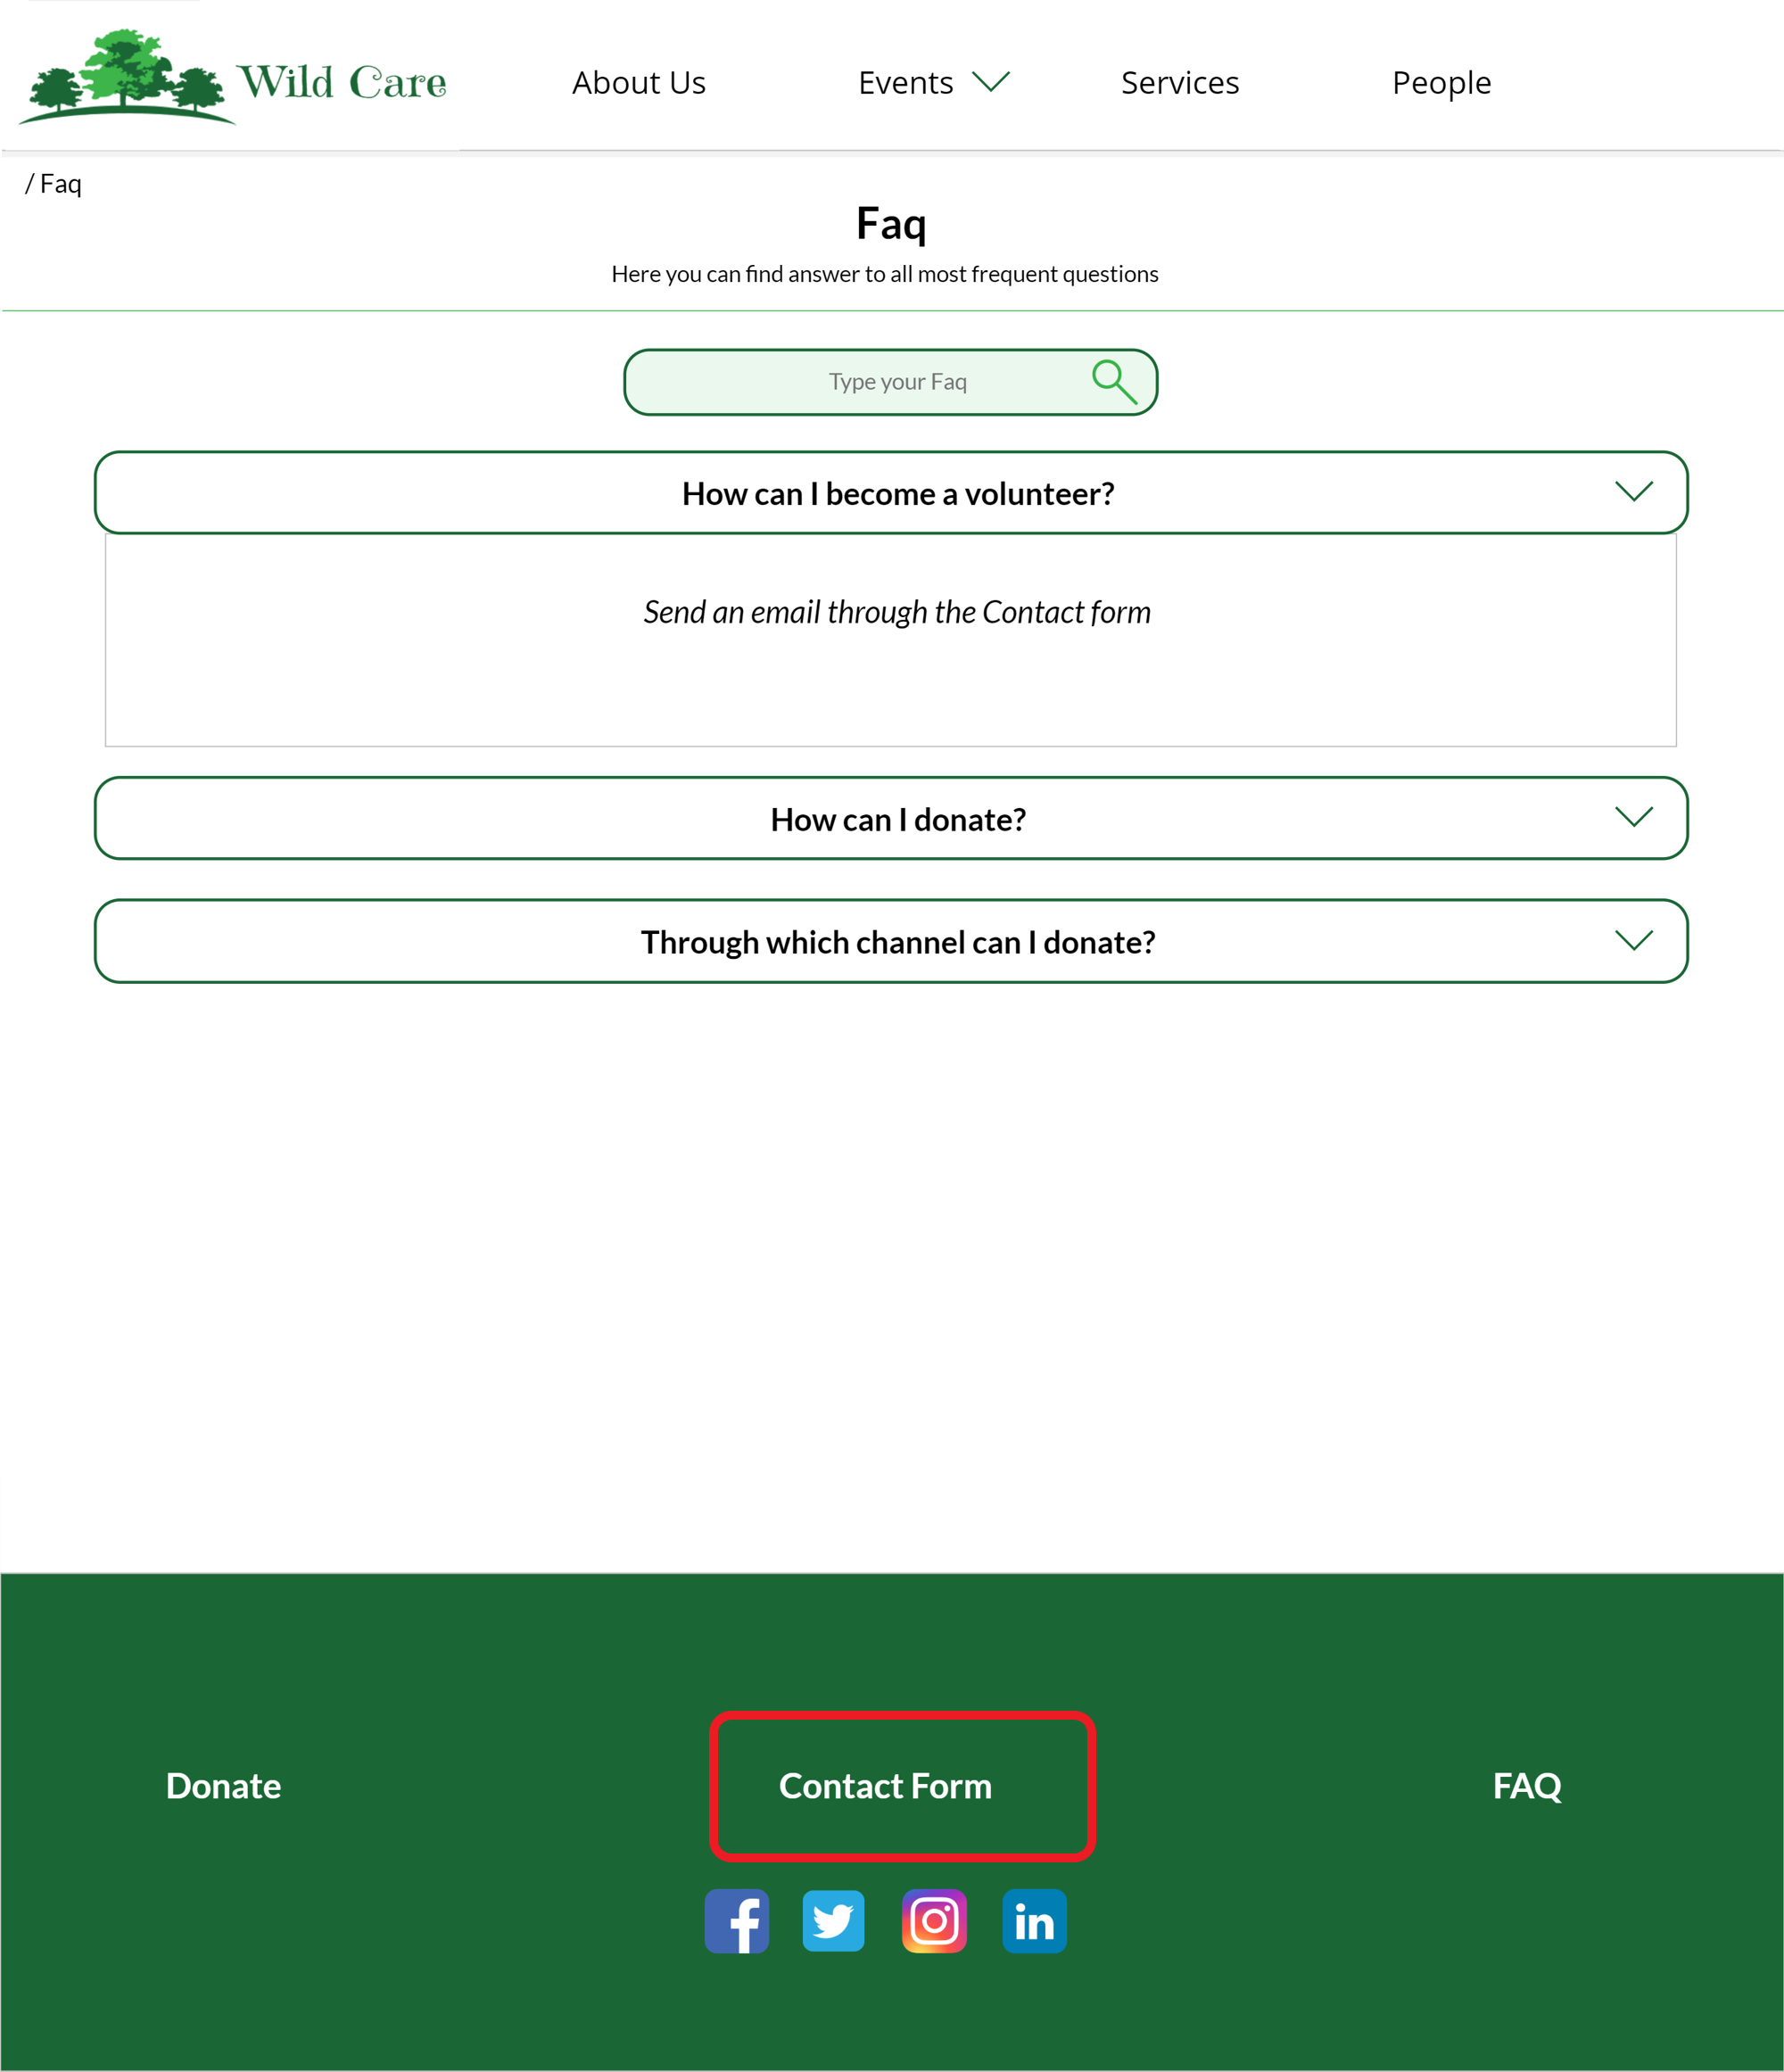
\includegraphics[width=\textwidth]{./assets/mockups/faq_contactform.png}
			\caption{Selects contact form.}
		\end{minipage}
	\end{figure}

	\begin{figure}[h!]
		\centering
		\begin{minipage}[b]{1\textwidth}
    			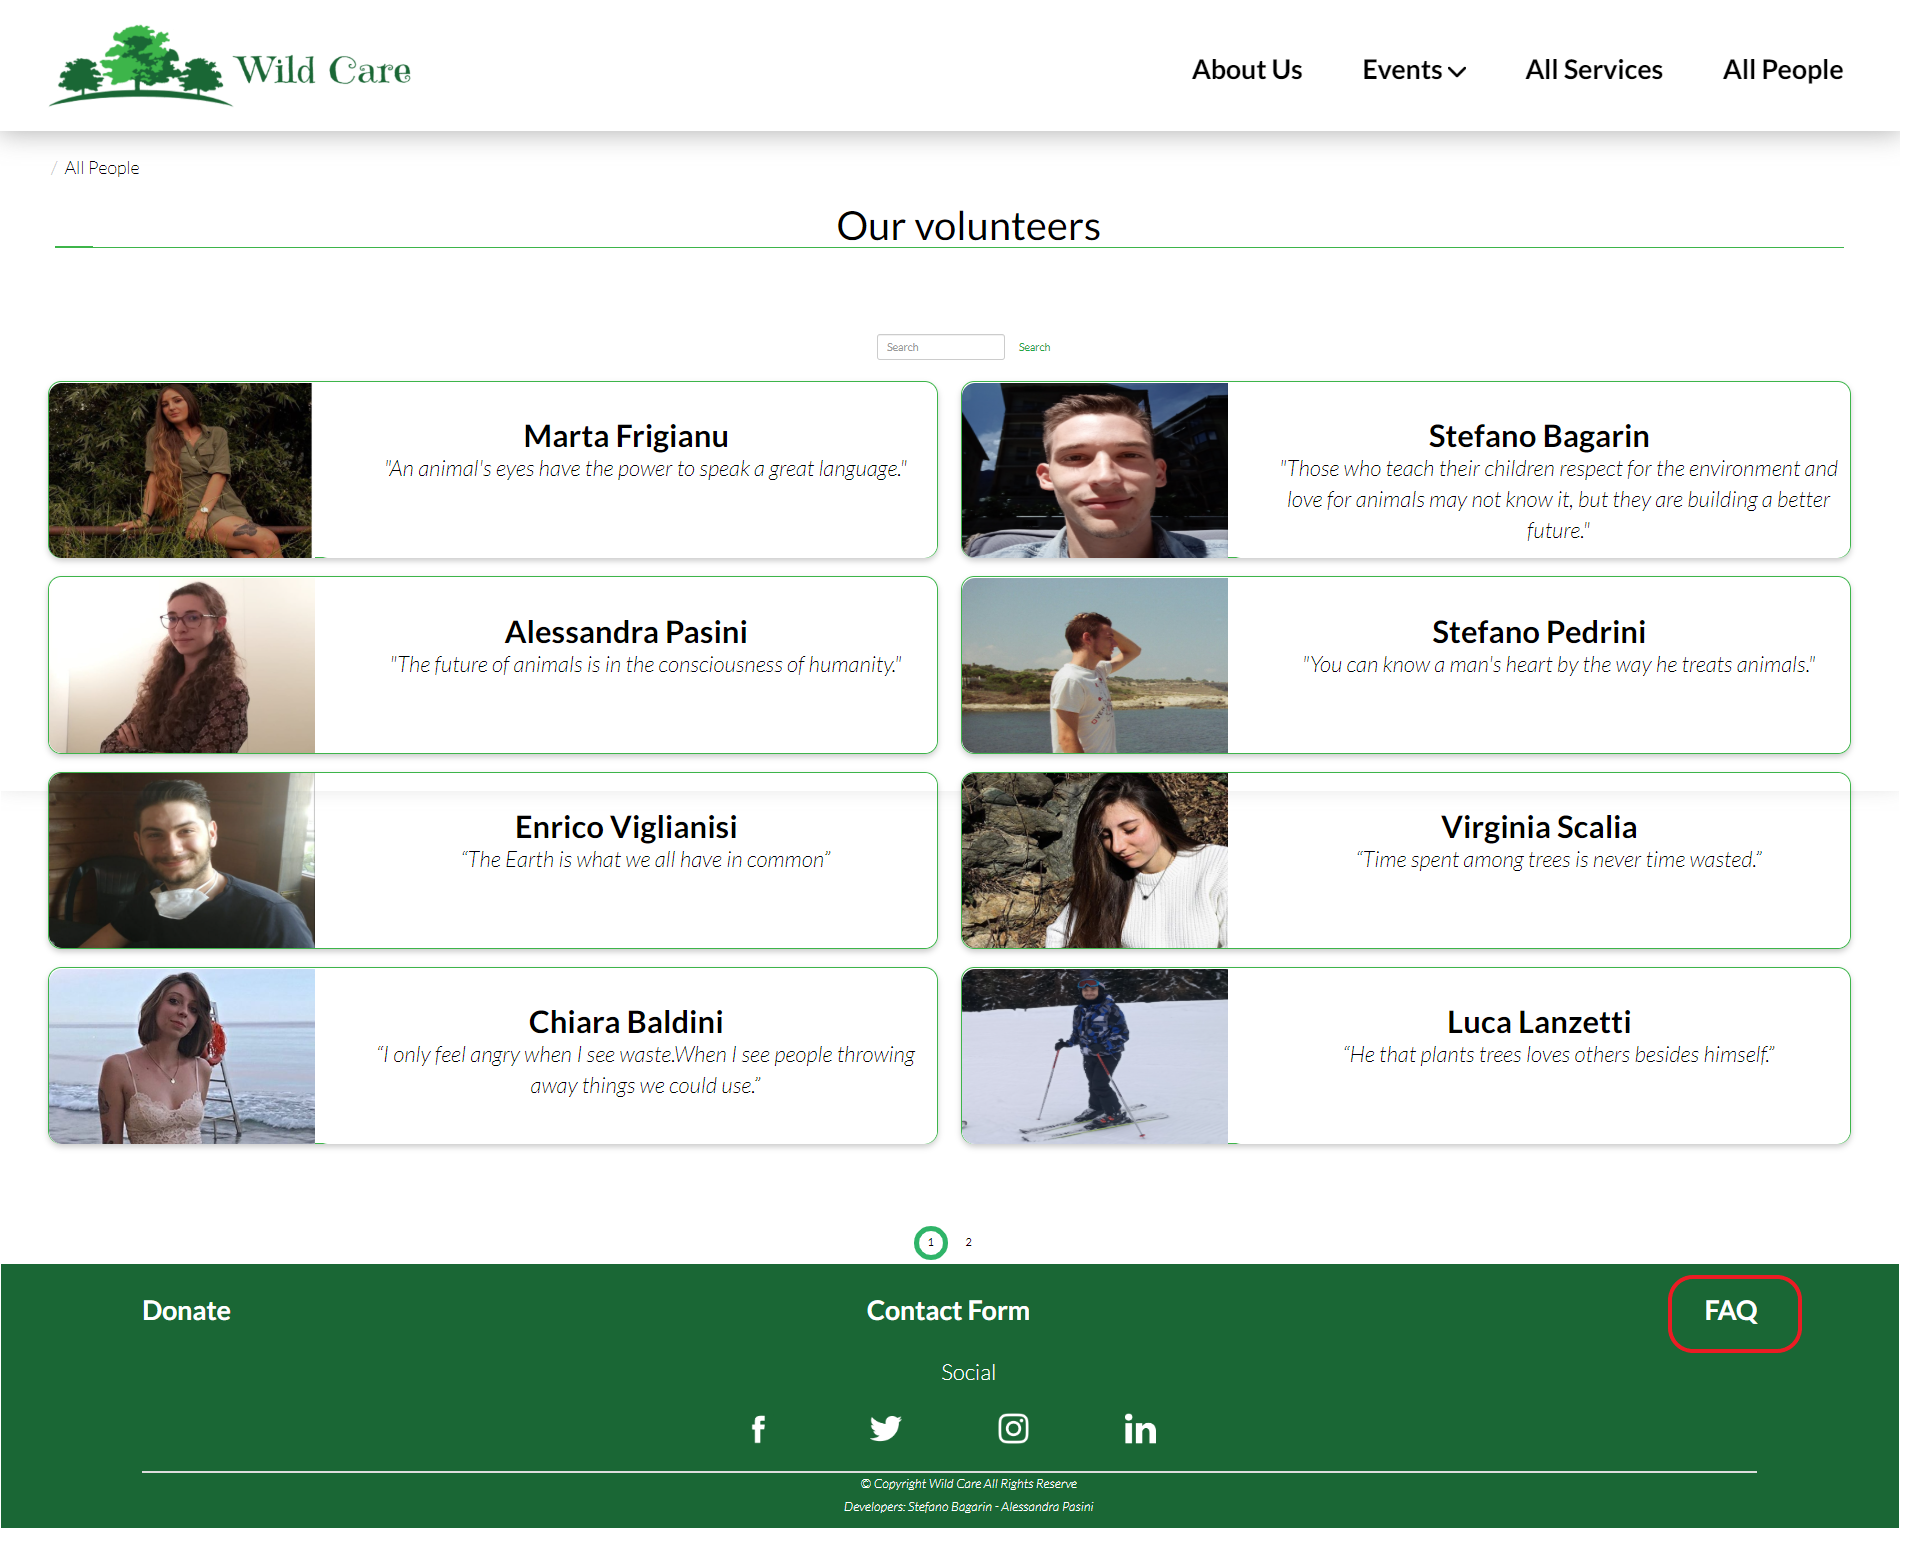
\includegraphics[width=\textwidth]{./assets/mockups/people_faq.png}
			\caption{Sends a message to the association.}
		\end{minipage}
	\end{figure}
\clearpage

	\subsection{Case 3}
	Stefano enjoys participating to some of the events organized by Wild Care sometimes. In particular, last week he took part to an event that offered a service about owls and he really liked both the content of the service and the interactiveness with the involved volunteers.\\
He decides to experience that again with he's girlfriend, so he connects to the website and starts to looking for that service with the volunteers that was involved last time too. When he finds it, he navigates to the next event that will offer it and reads when it's going to take place.

	\begin{figure}[h!]
		\centering
		\begin{minipage}[b]{0.8\textwidth}
    			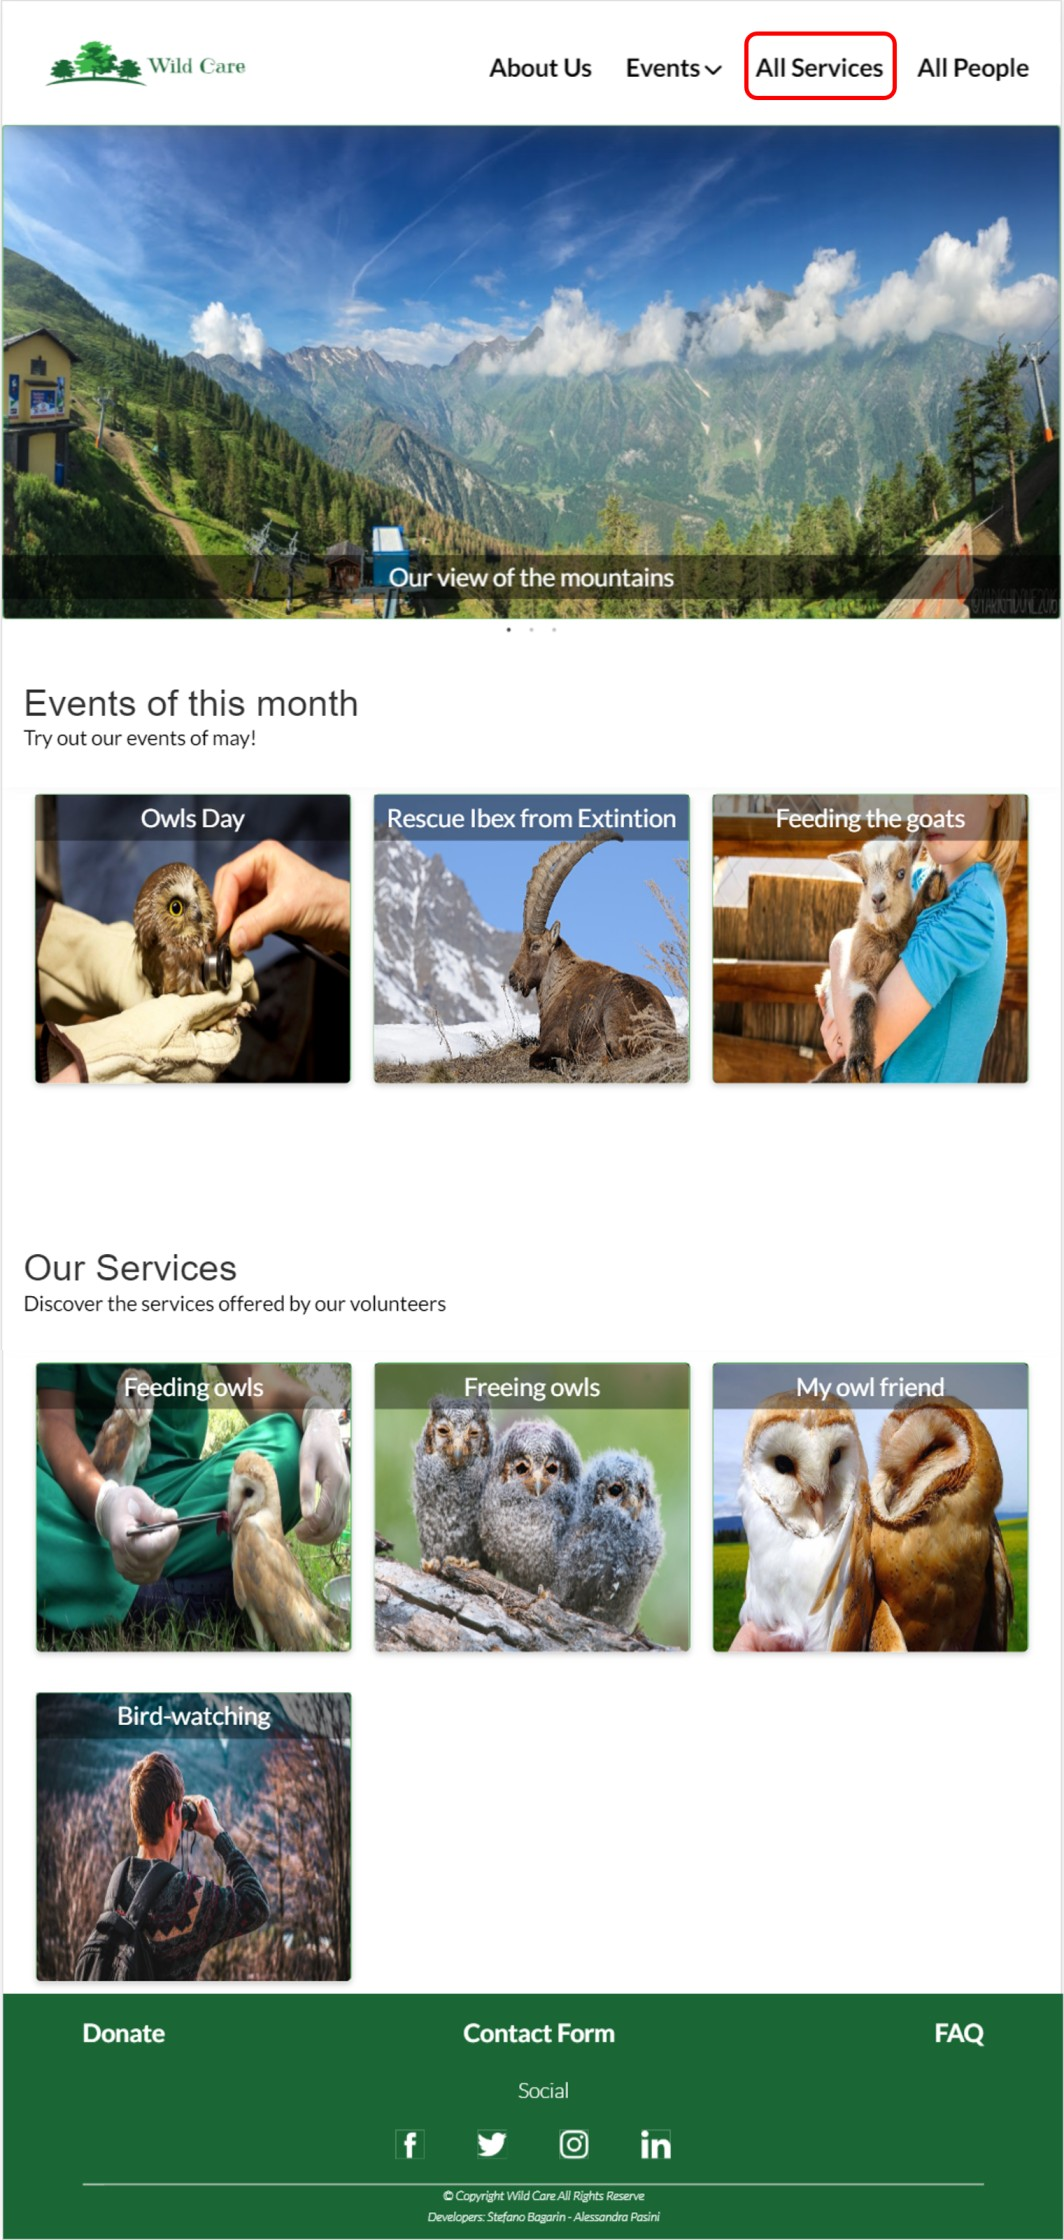
\includegraphics[width= \textwidth]{./assets/mockups/homepage_services.jpg}
			\caption{Selects services from the home page.}
		\end{minipage}
	\end{figure}

	\begin{figure}[h!]
		\centering
		\begin{minipage}[b]{1\textwidth}
    			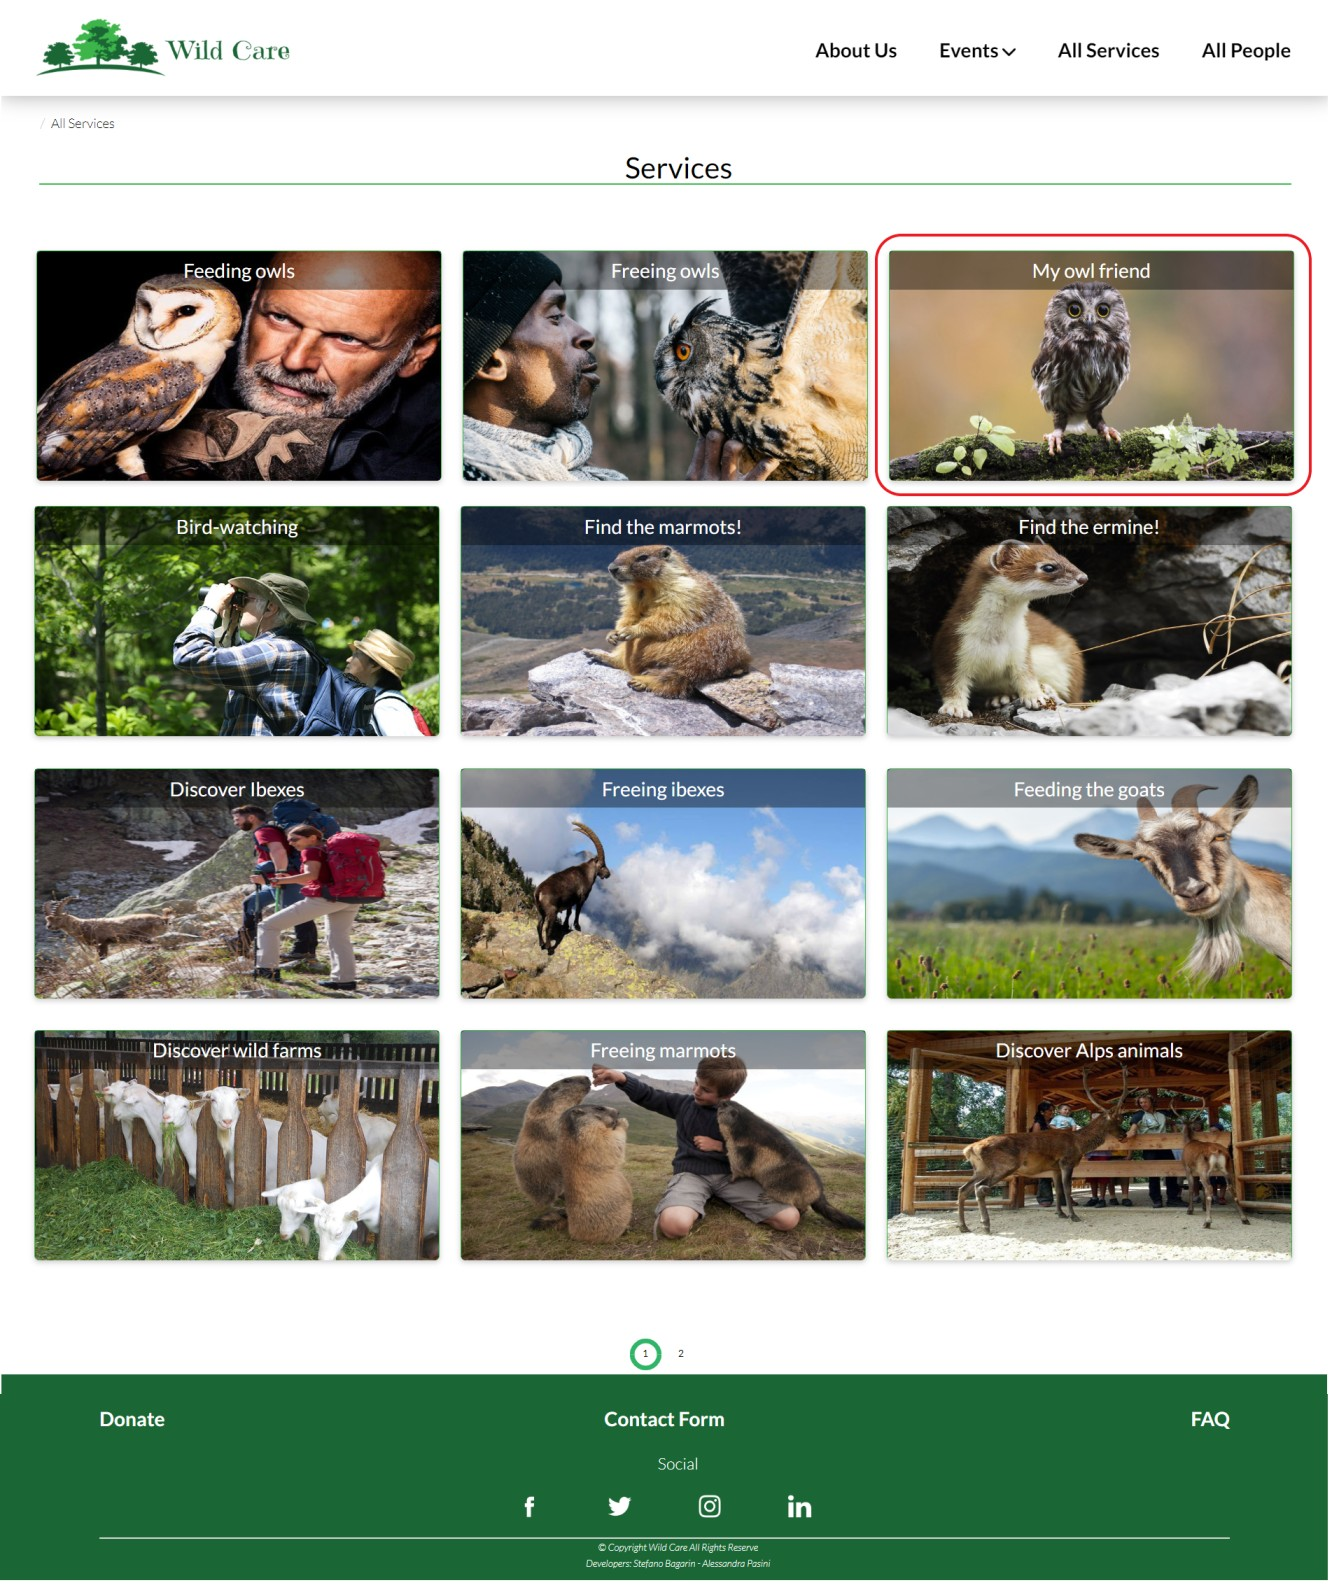
\includegraphics[width=\textwidth]{./assets/mockups/services_servicedetails.jpg}
			\caption{Selects the service.}
		\end{minipage}
	\end{figure}

	\begin{figure}[h!]
		\centering
		\begin{minipage}[b]{1\textwidth}
    			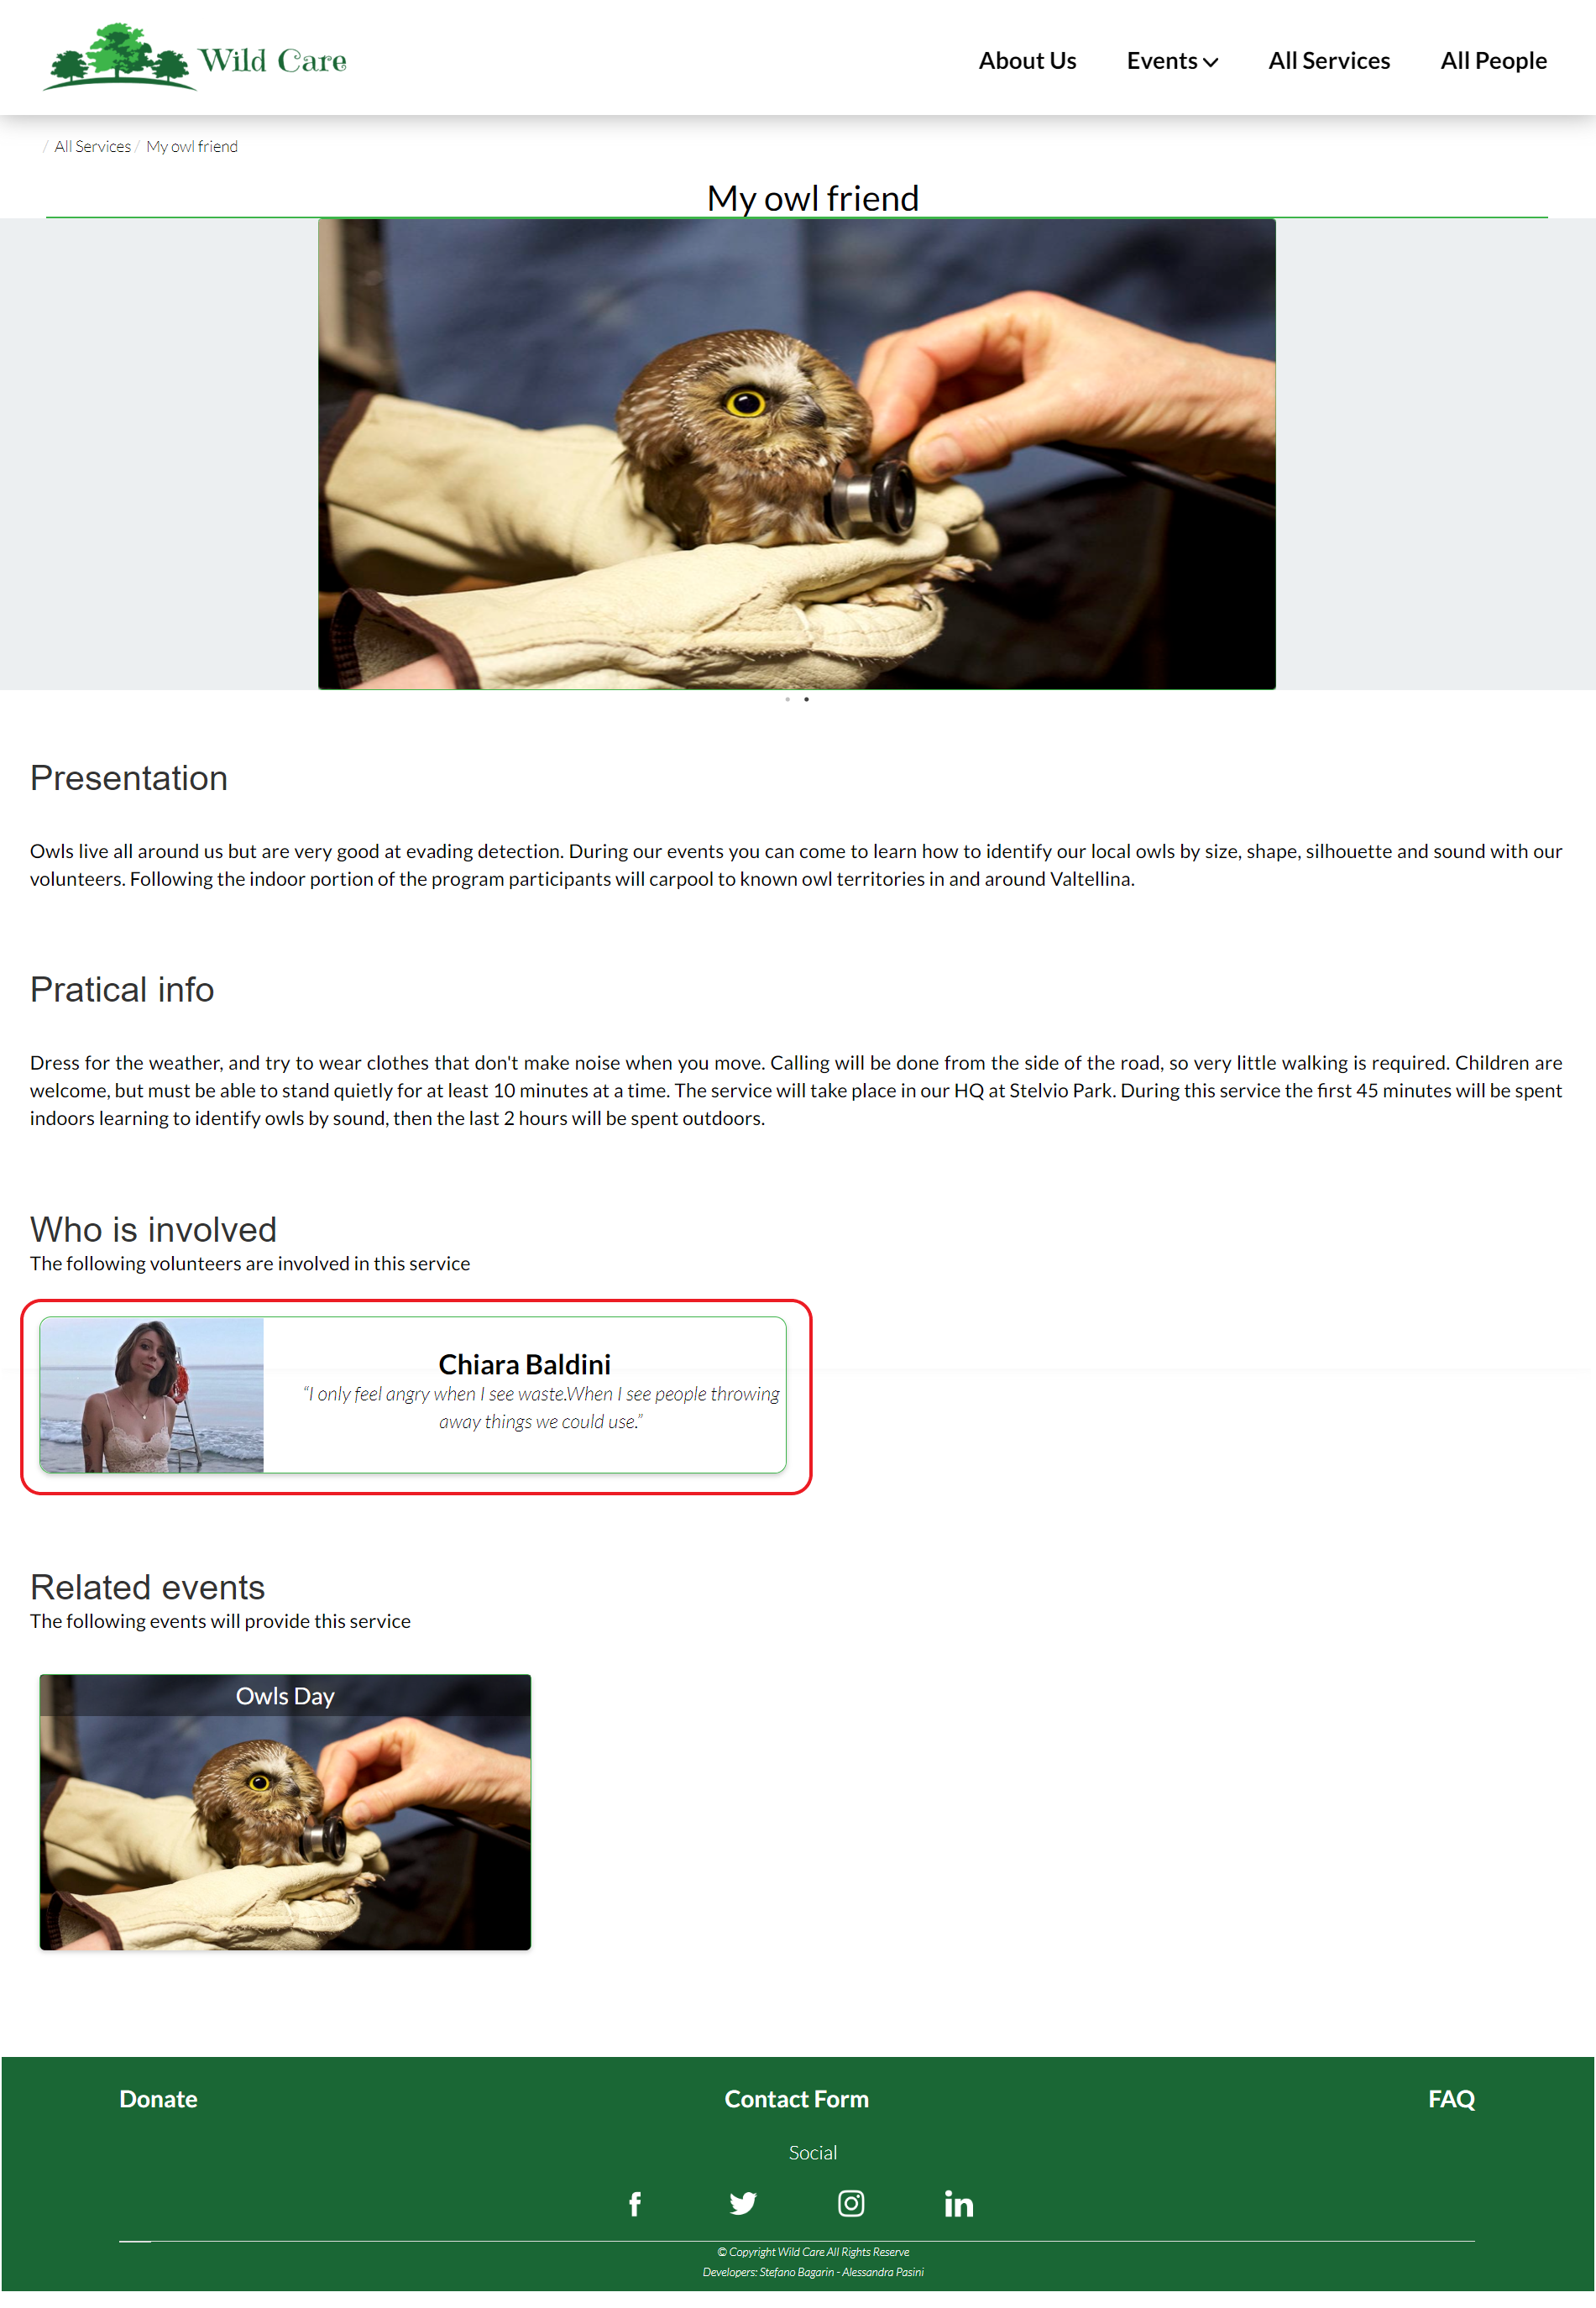
\includegraphics[width=\textwidth]{./assets/mockups/servicedetails_persondetails.png}
			\caption{Checks the volunteers.}
		\end{minipage}
	\end{figure}

	\begin{figure}[h!]
		\centering
		\begin{minipage}[b]{1\textwidth}
    			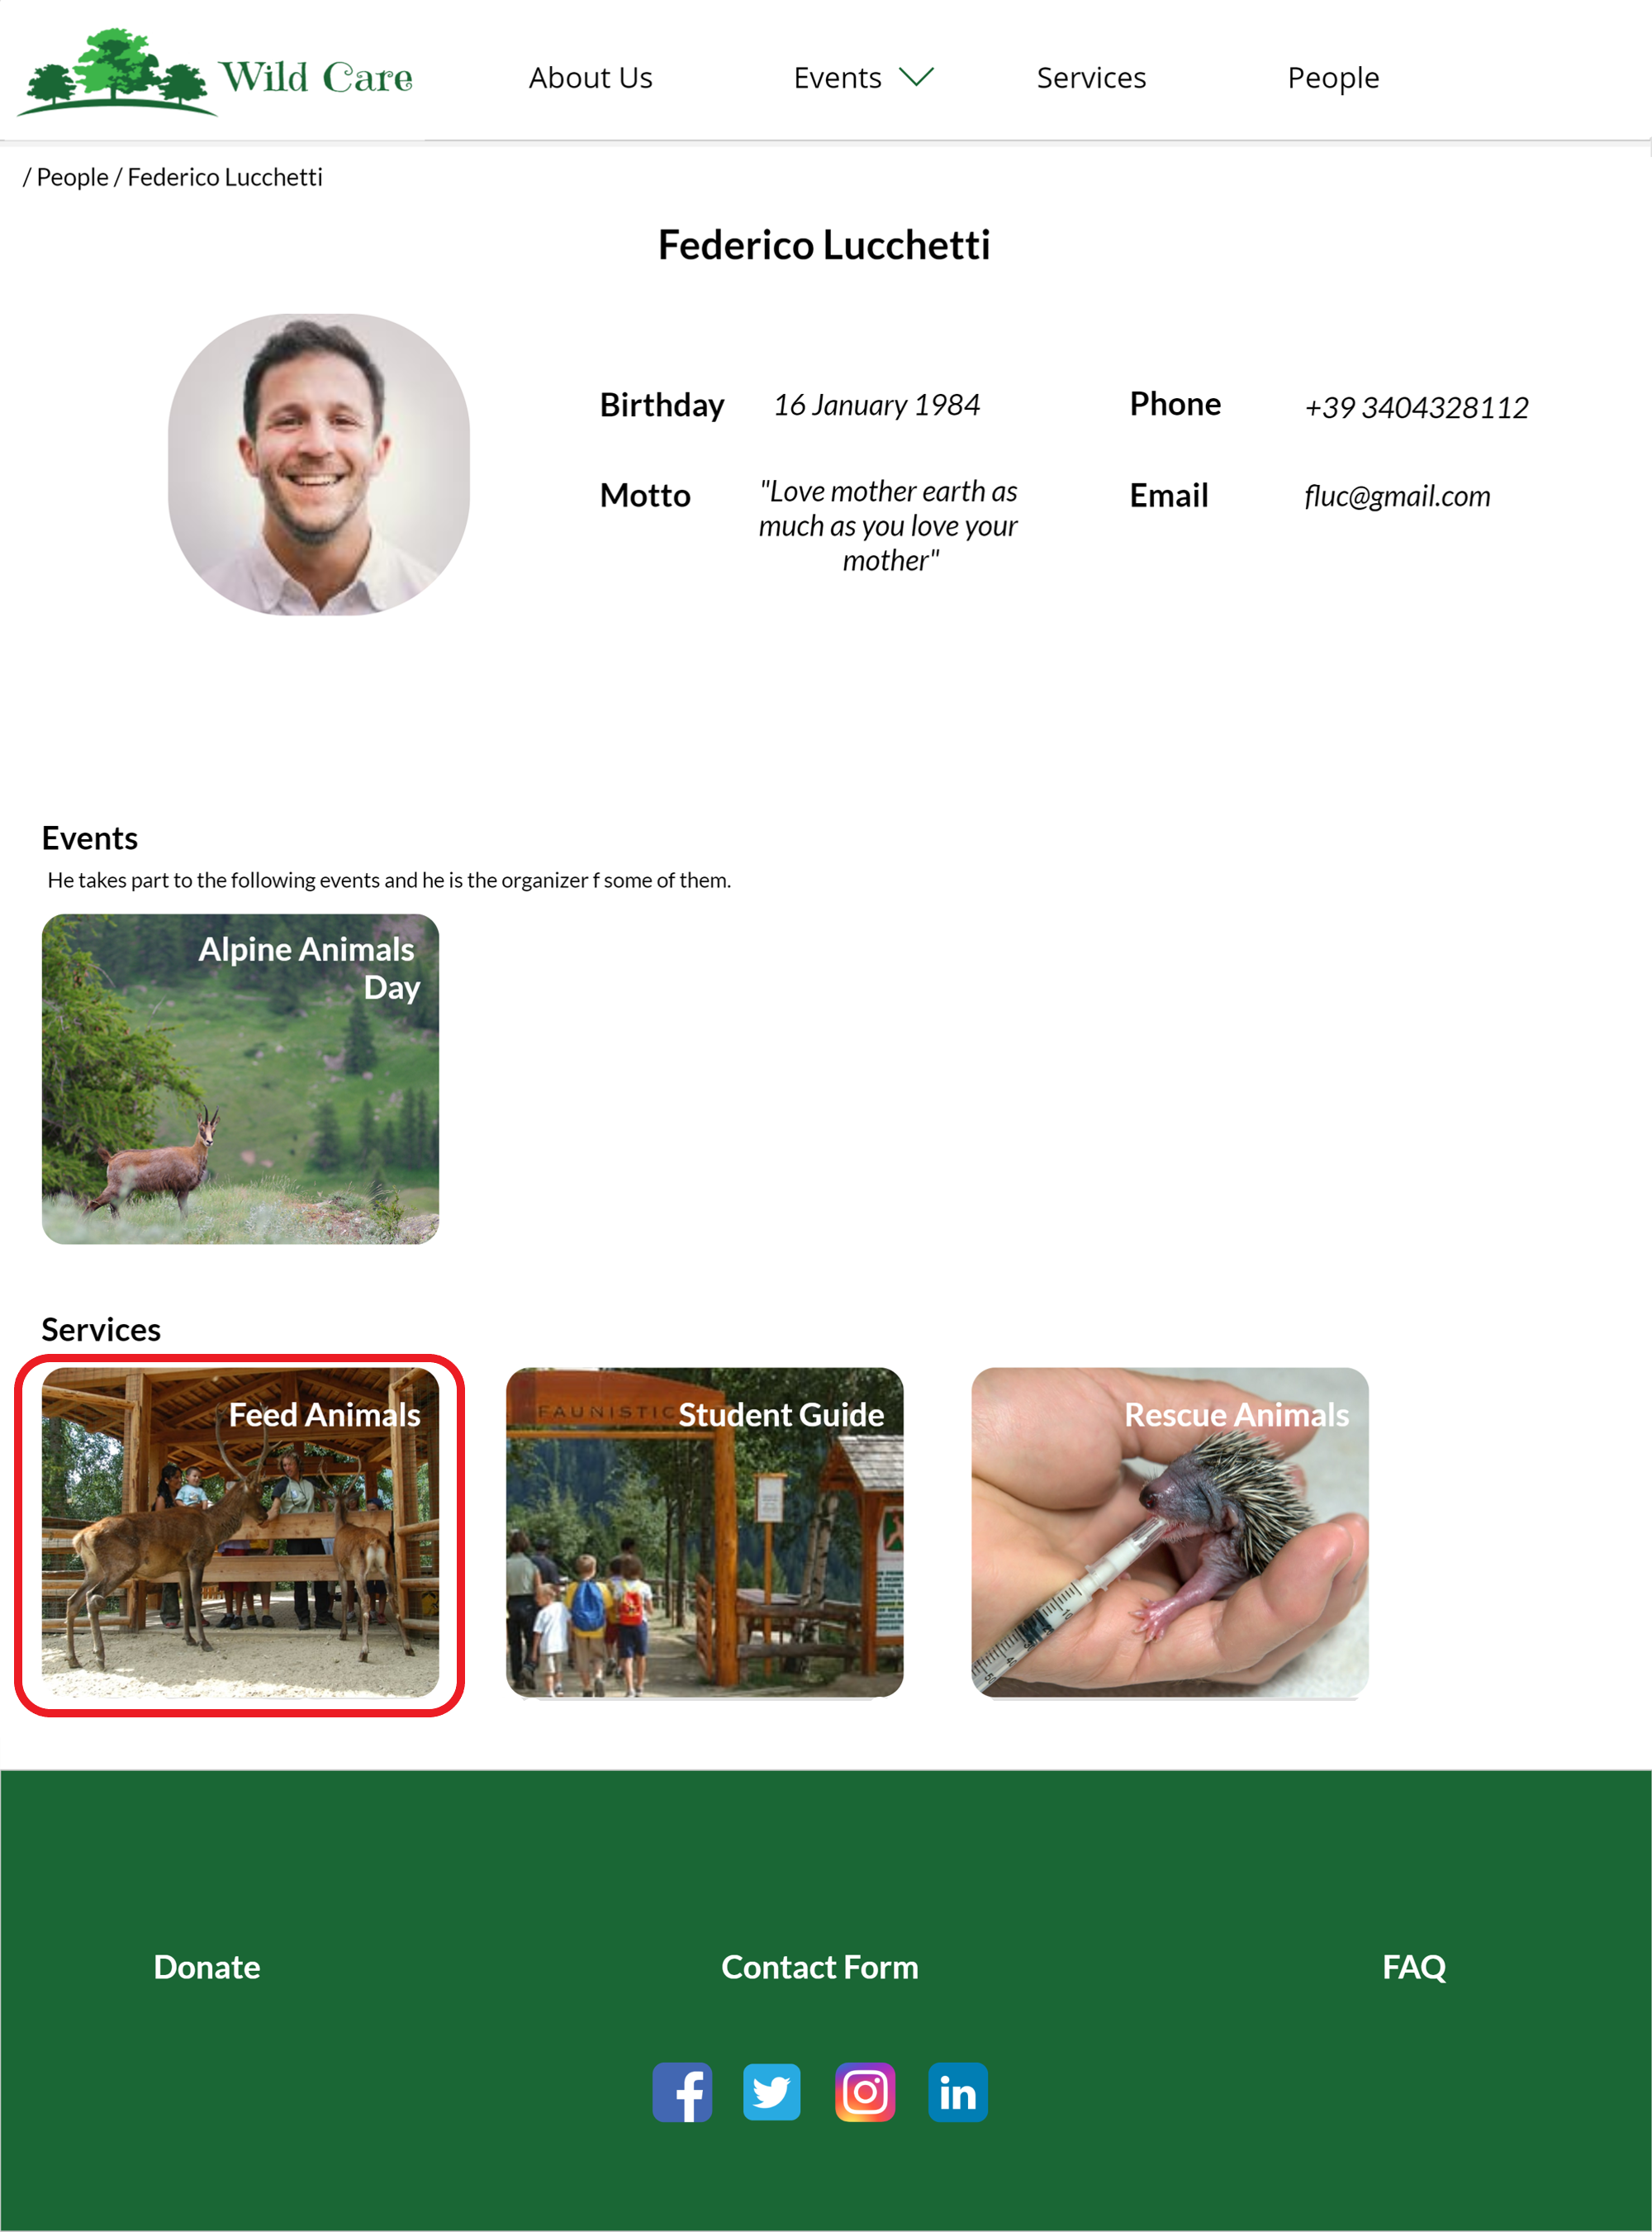
\includegraphics[width=\textwidth]{./assets/mockups/persondetails_servicedetails.png}
			\caption{Goes back to the service page.}
		\end{minipage}
	\end{figure}

	\begin{figure}[h!]
		\centering
		\begin{minipage}[b]{1\textwidth}
    			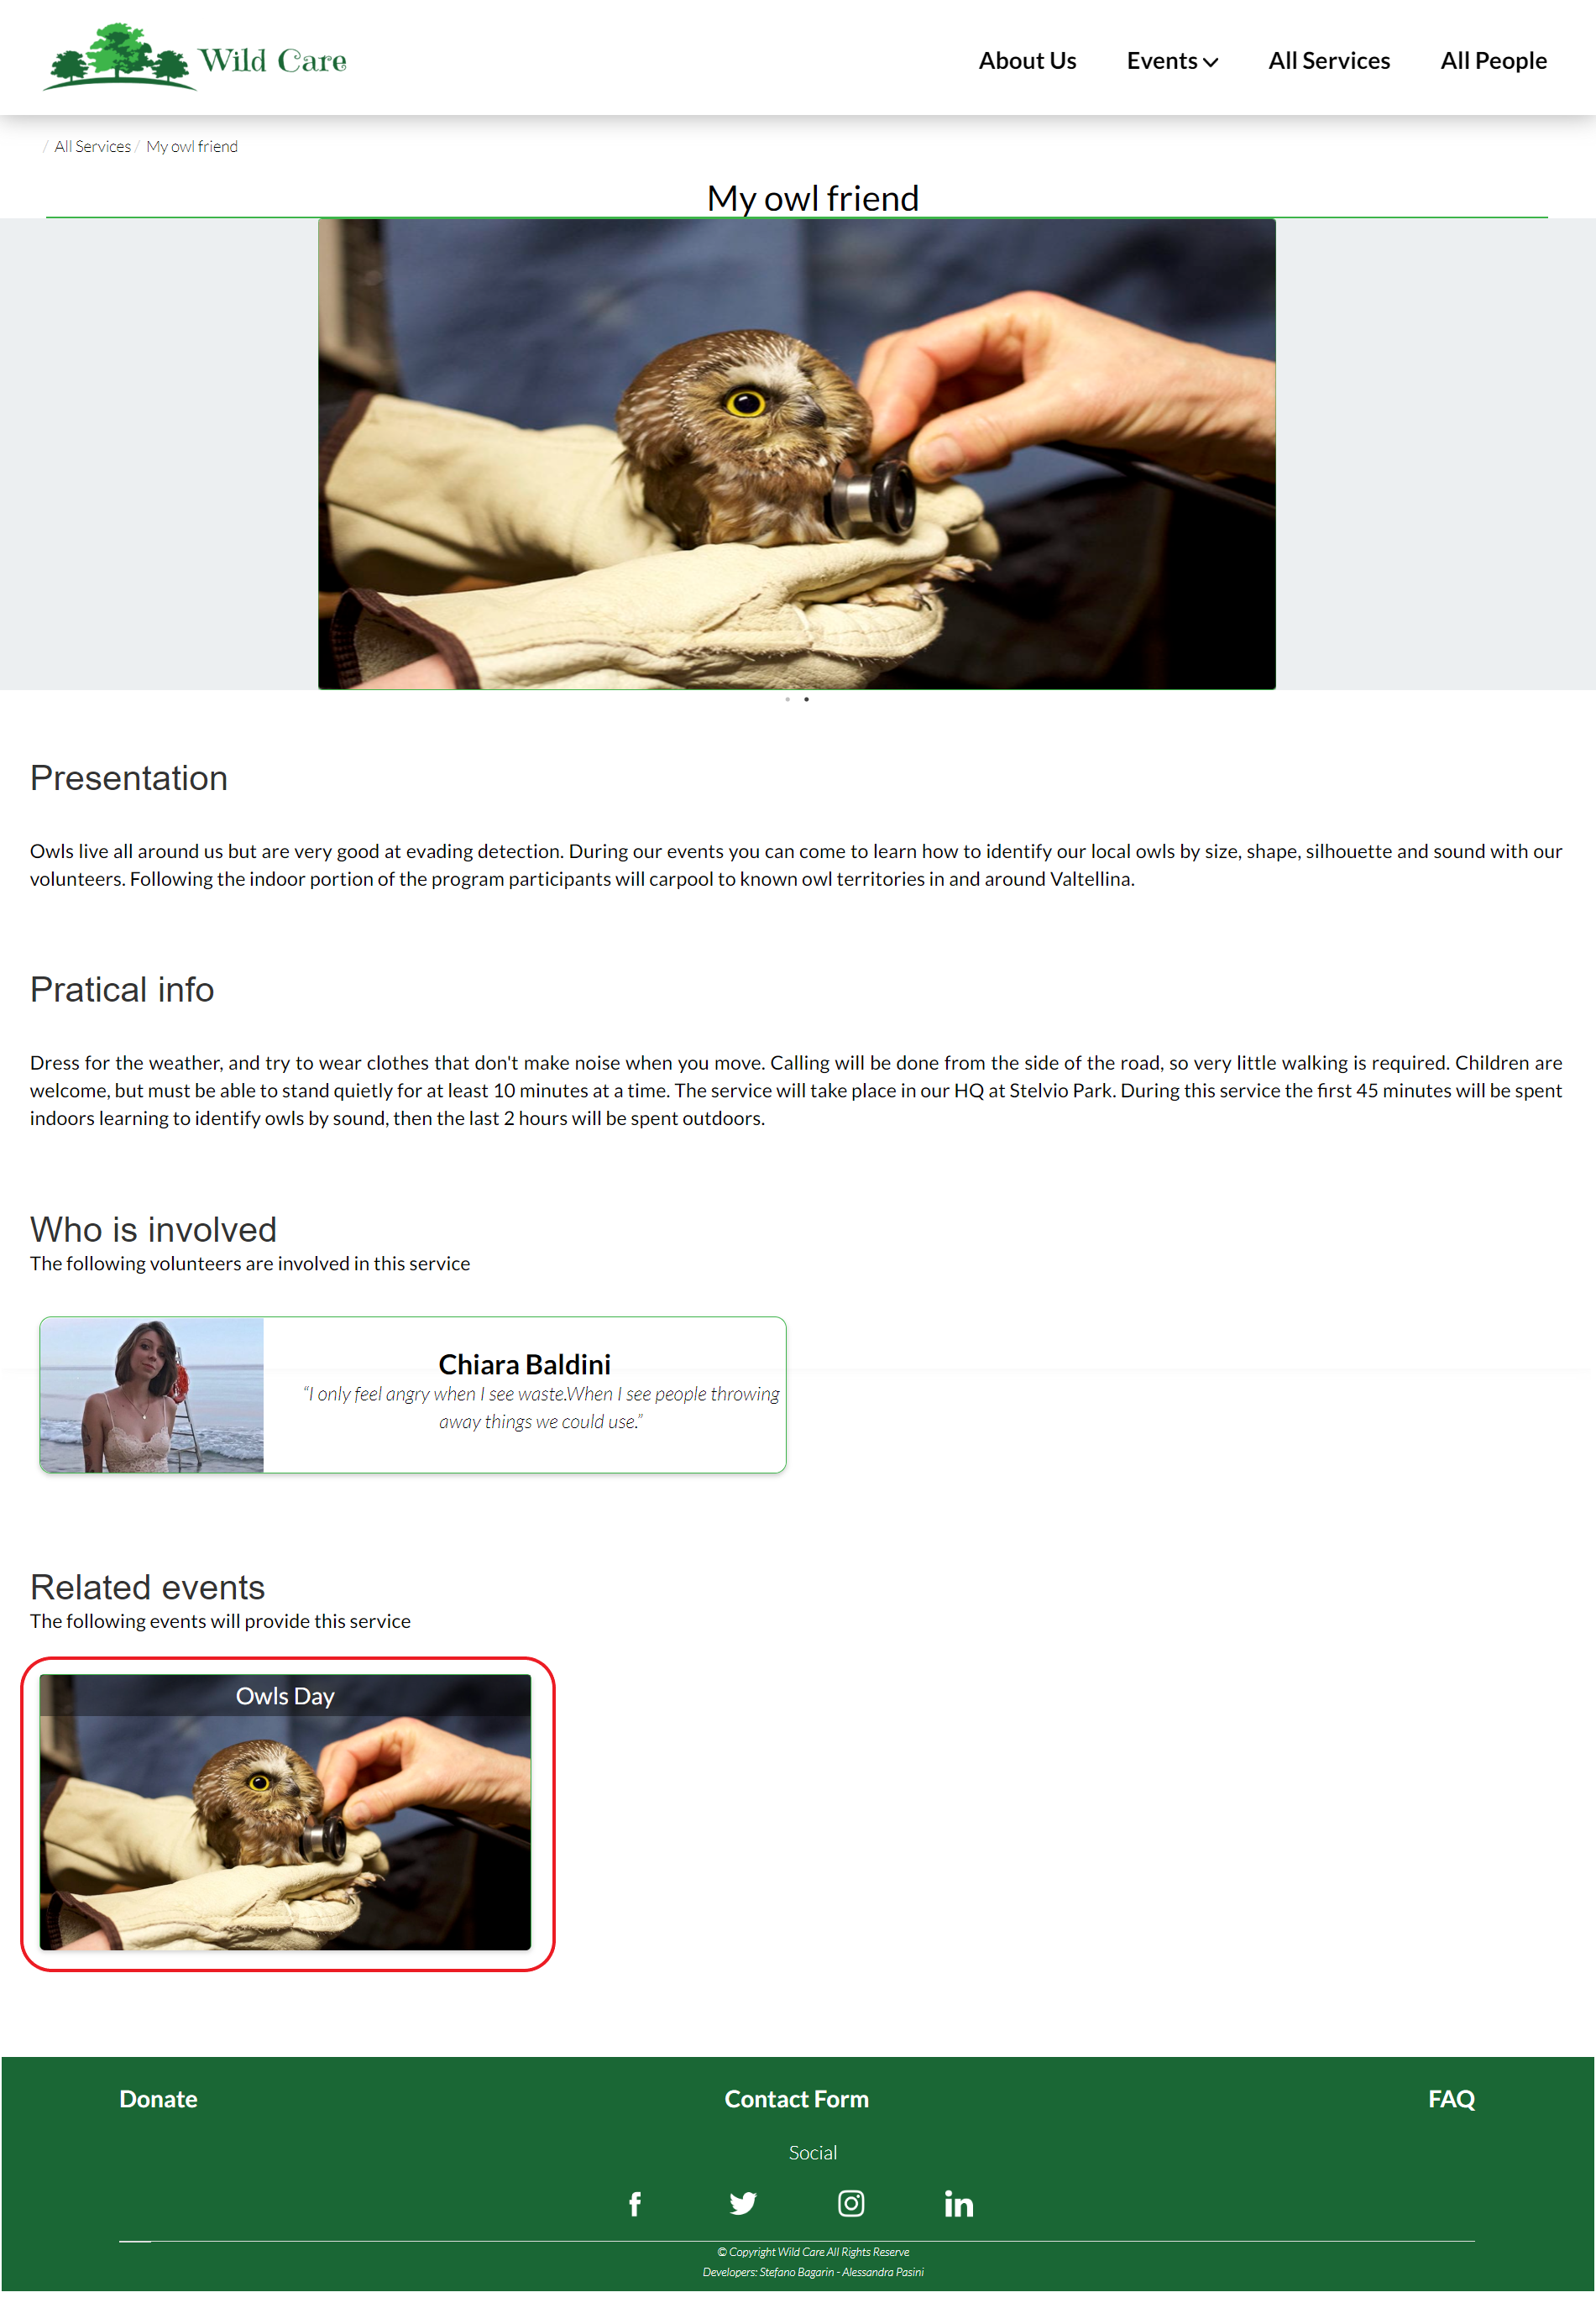
\includegraphics[width=\textwidth]{./assets/mockups/servicedetails_eventdetails.png}
			\caption{Navigates to the related event page.}
		\end{minipage}
	\end{figure}

	\begin{figure}[h!]
		\centering
		\begin{minipage}[b]{1\textwidth}
    			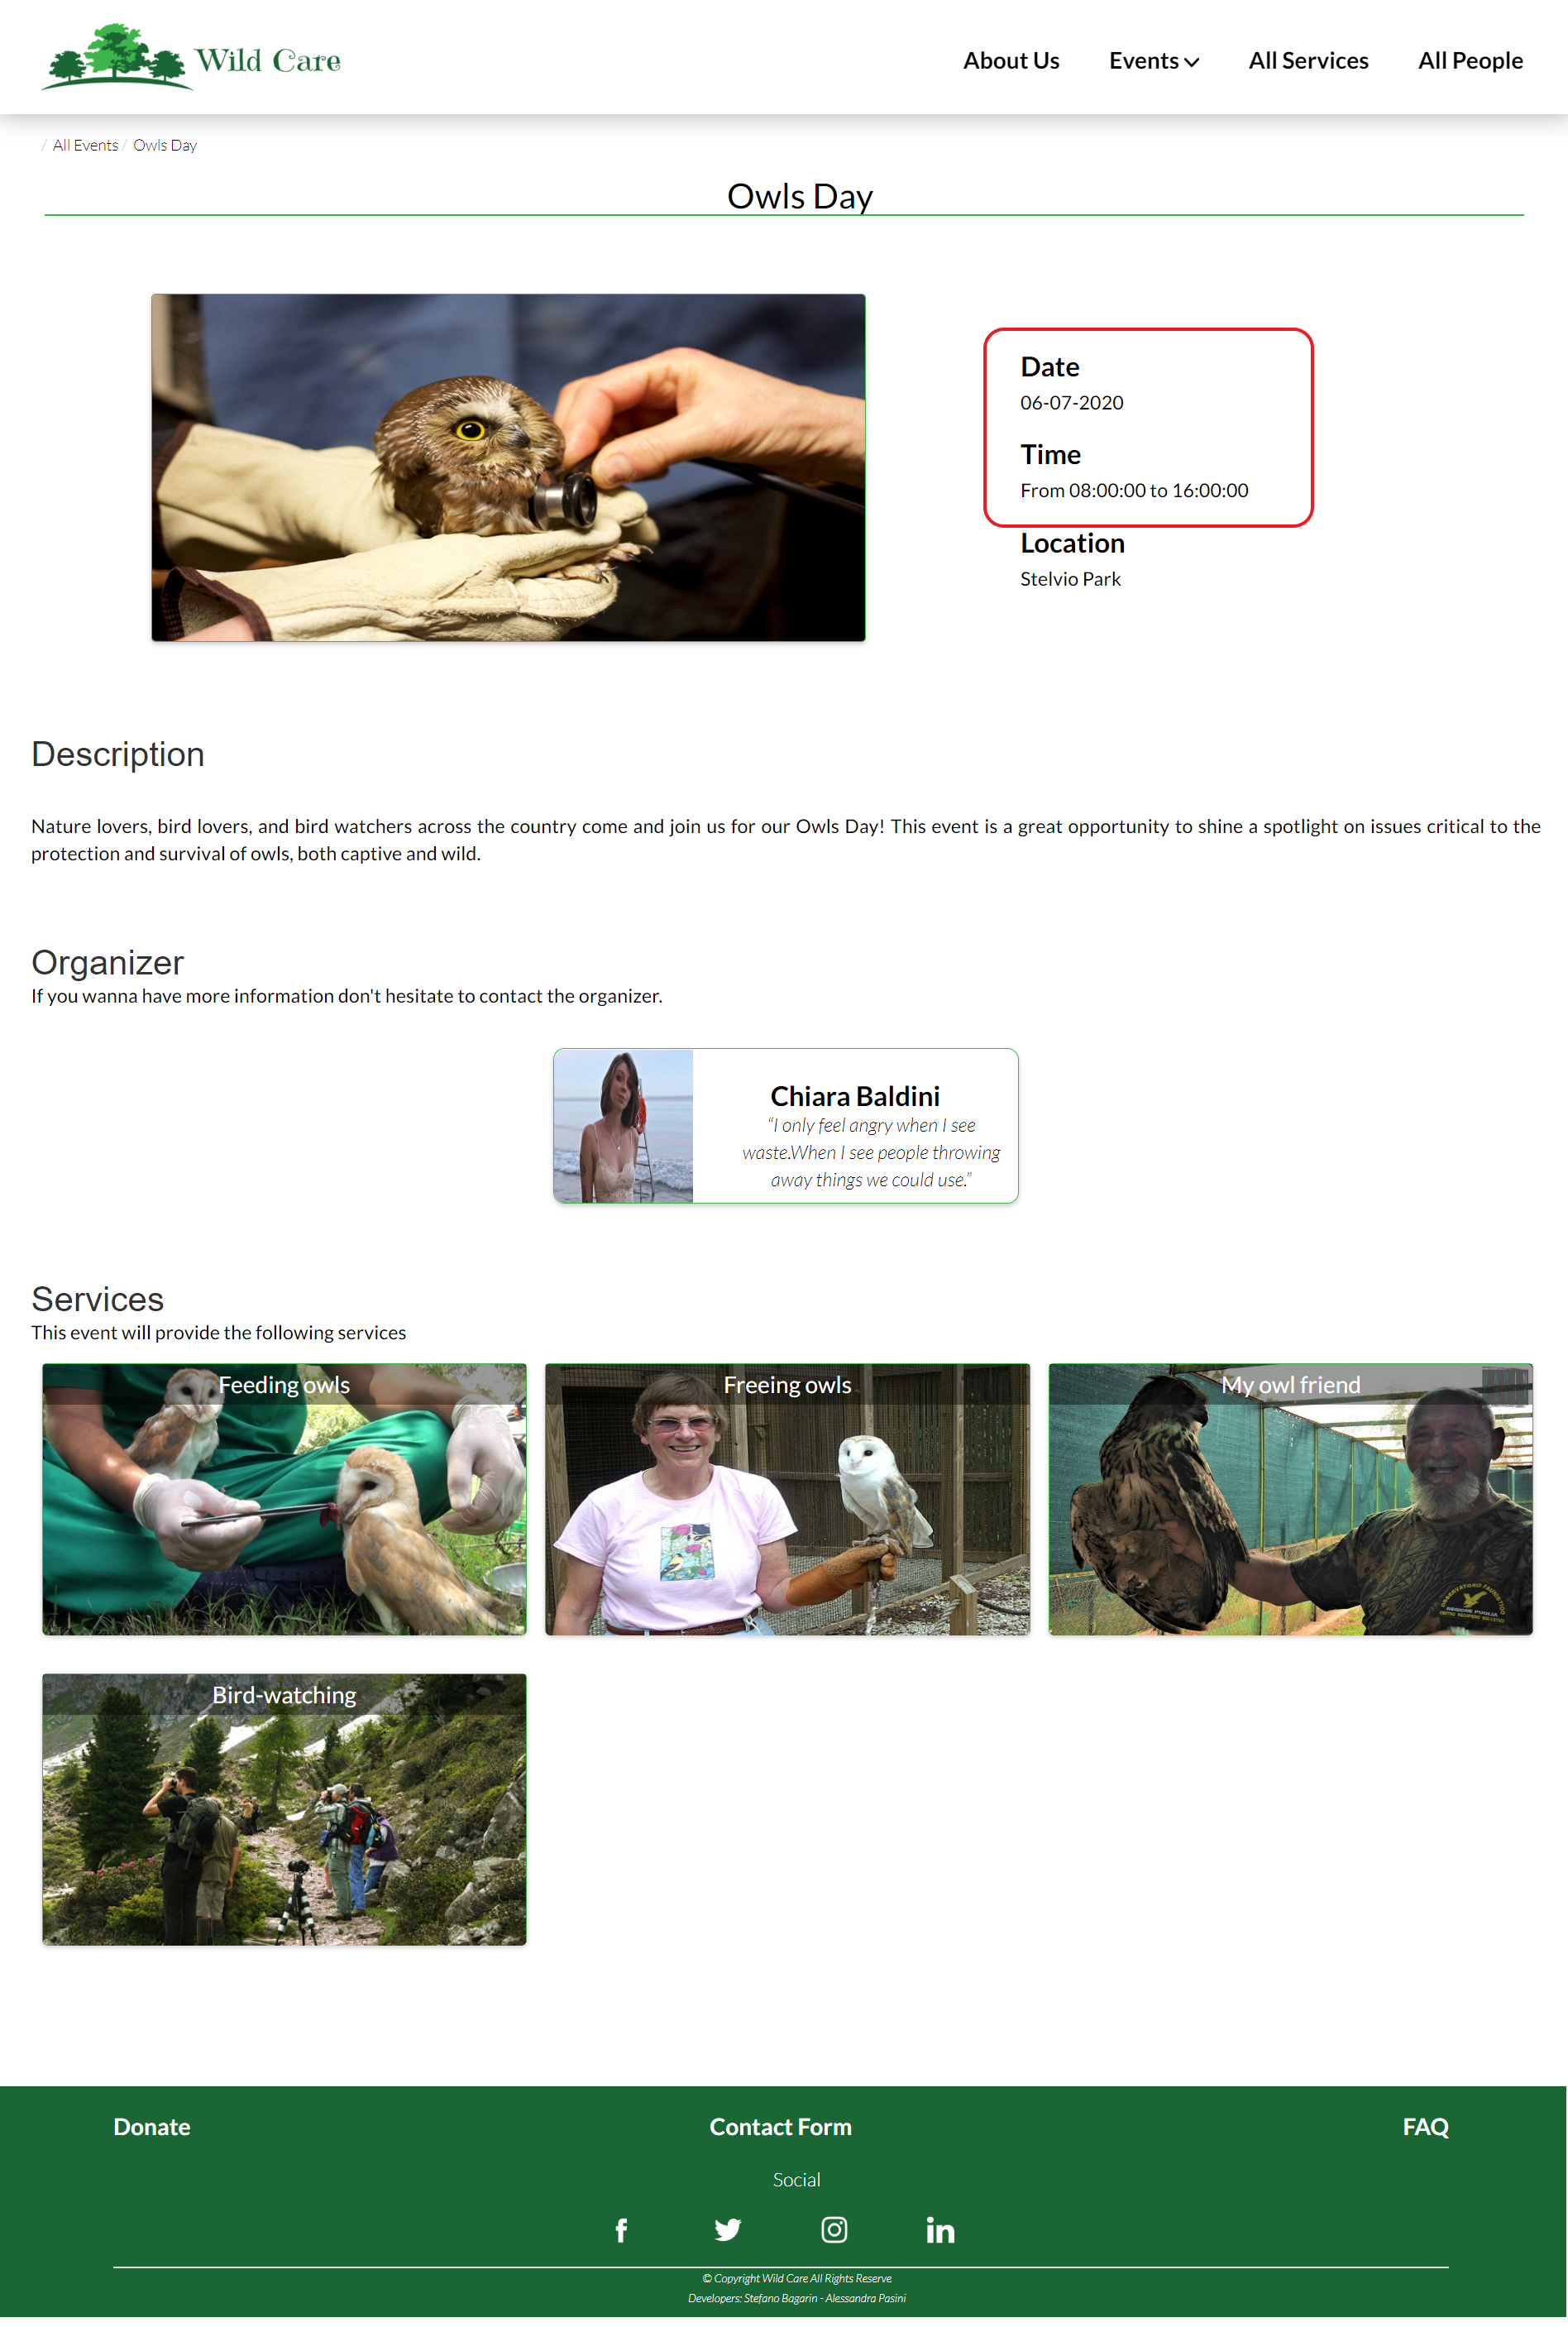
\includegraphics[width=\textwidth]{./assets/mockups/eventdetails_date.png}
			\caption{checks when the event will take place.}
		\end{minipage}
	\end{figure}

	\clearpage


	%Design in-the-small
	\section{Design in-the-small}

	\subsection{Home Page}
	The association's homepage gives a general representation of the main websites's categories.  TODOIt alsco contains links to sSome useful links are provided in order to easily reach subsets of
books or events, for instance is possible to fetch best seller books or latest event
just with one click. In order to make the navigation smoother and the website more
user friendly, the home page contains some Carousel slideshow.

\begin{figure}[h!]
	\centering
	\begin{minipage}[b]{1\textwidth}
    		\includegraphics[width=\textwidth]{./assets/homepage.png}
		\caption{Homepage in the small}
	\end{minipage}
\end{figure}
\FloatBarrier



	\clearpage

	\subsection{About us}
	This is the page dedicated to describe and give general information about our association. It is formed by 4 main sections: 
\begin{itemize}
	\item \textbf{Who we are: } gives genral info about the association
	\item \textbf{Our Mission: } explains the purpose and final scope
	\item \textbf{History: } tells to user what the association as done from the foundation to today
	\item \textbf{FAQ: } contains some common questions and related answers
\end{itemize}
A set of functional links has been added to let users easily navigate between these sections.

\begin{figure}[h!]
	\centering
	\begin{minipage}[b]{1\textwidth}
    		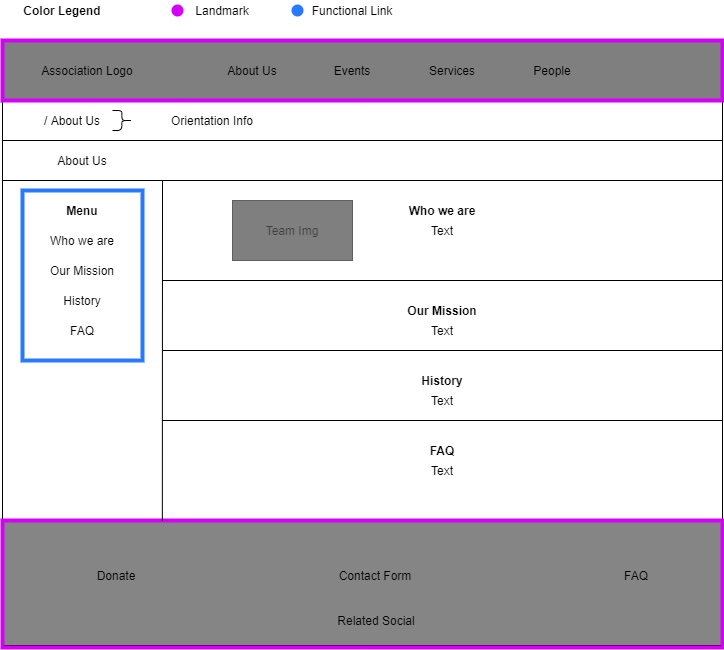
\includegraphics[width=\textwidth]{./assets/aboutus.png}
		\caption{About Us page - Design in the small}
	\end{minipage}
\end{figure}
\FloatBarrier
\clearpage


\subsection{Contact Form}
The aim of this page is to let users ask quetions or send messages to association's info email through a contact form, whose fields are all mandatory. \\
Once filled the fom, Send button must be clicked:
\begin{itemize}
	\item if one or more fields are empty or if the email is invalid (being valid means that it has the following structure: 				\emph{example@example.com}) an error message will occur;
	\item if the form has been well completed a success message will pop up.
\end{itemize}

\begin{figure}[h!]
	\centering
	\begin{minipage}[b]{1\textwidth}
    		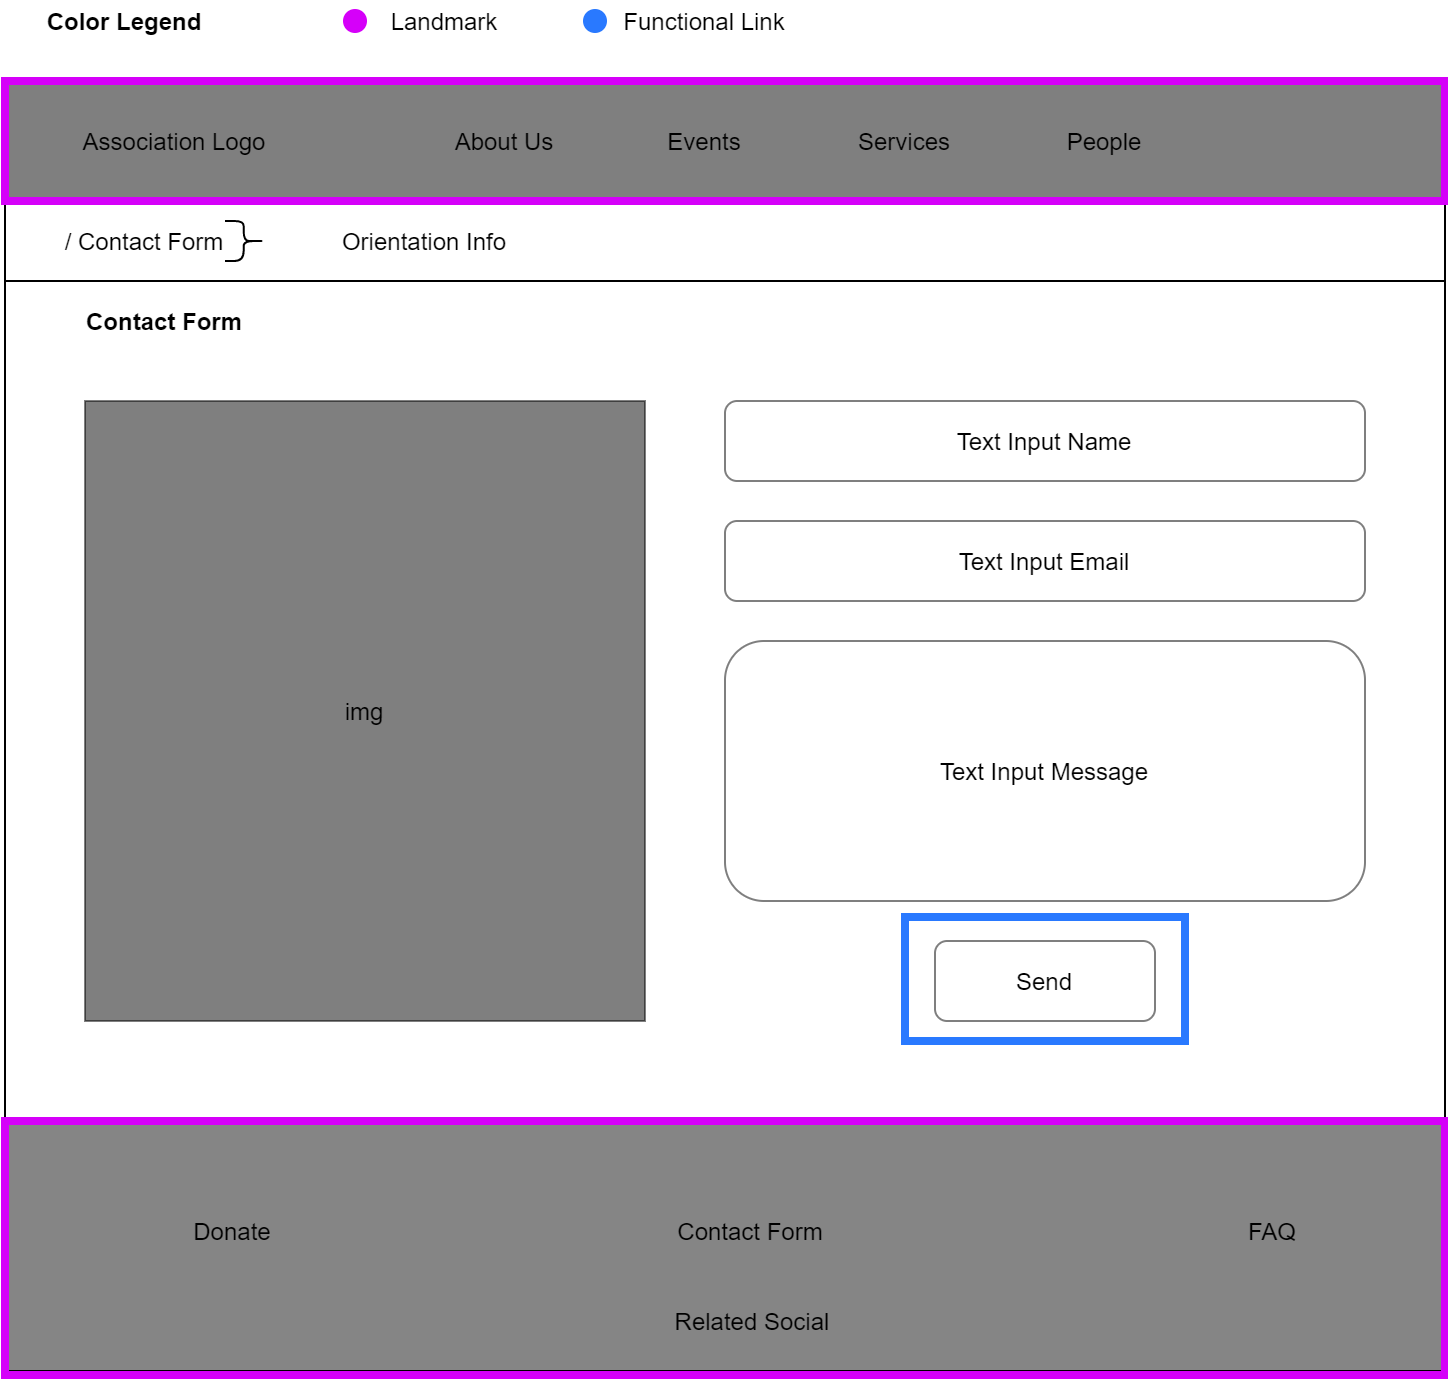
\includegraphics[width=\textwidth]{./assets/contactform.png}
		\caption{Contact Form page - Design in the small}
	\end{minipage}
\end{figure}
\FloatBarrier
	\clearpage

	\subsection{Events}
	The \emph{Events} page contains a grid with all events that our association organizes.  By clicking on each event image or name it is possible to navigate to the event's details page. Through the group links into the left side menu is possible to filter events depending on their type and date (the date filter is different from "Events by Month x" multiple group).

\subsubsection{Events in-the-small}
\begin{figure}[h!]
		\centering
		\begin{minipage}[b]{1\textwidth}
    			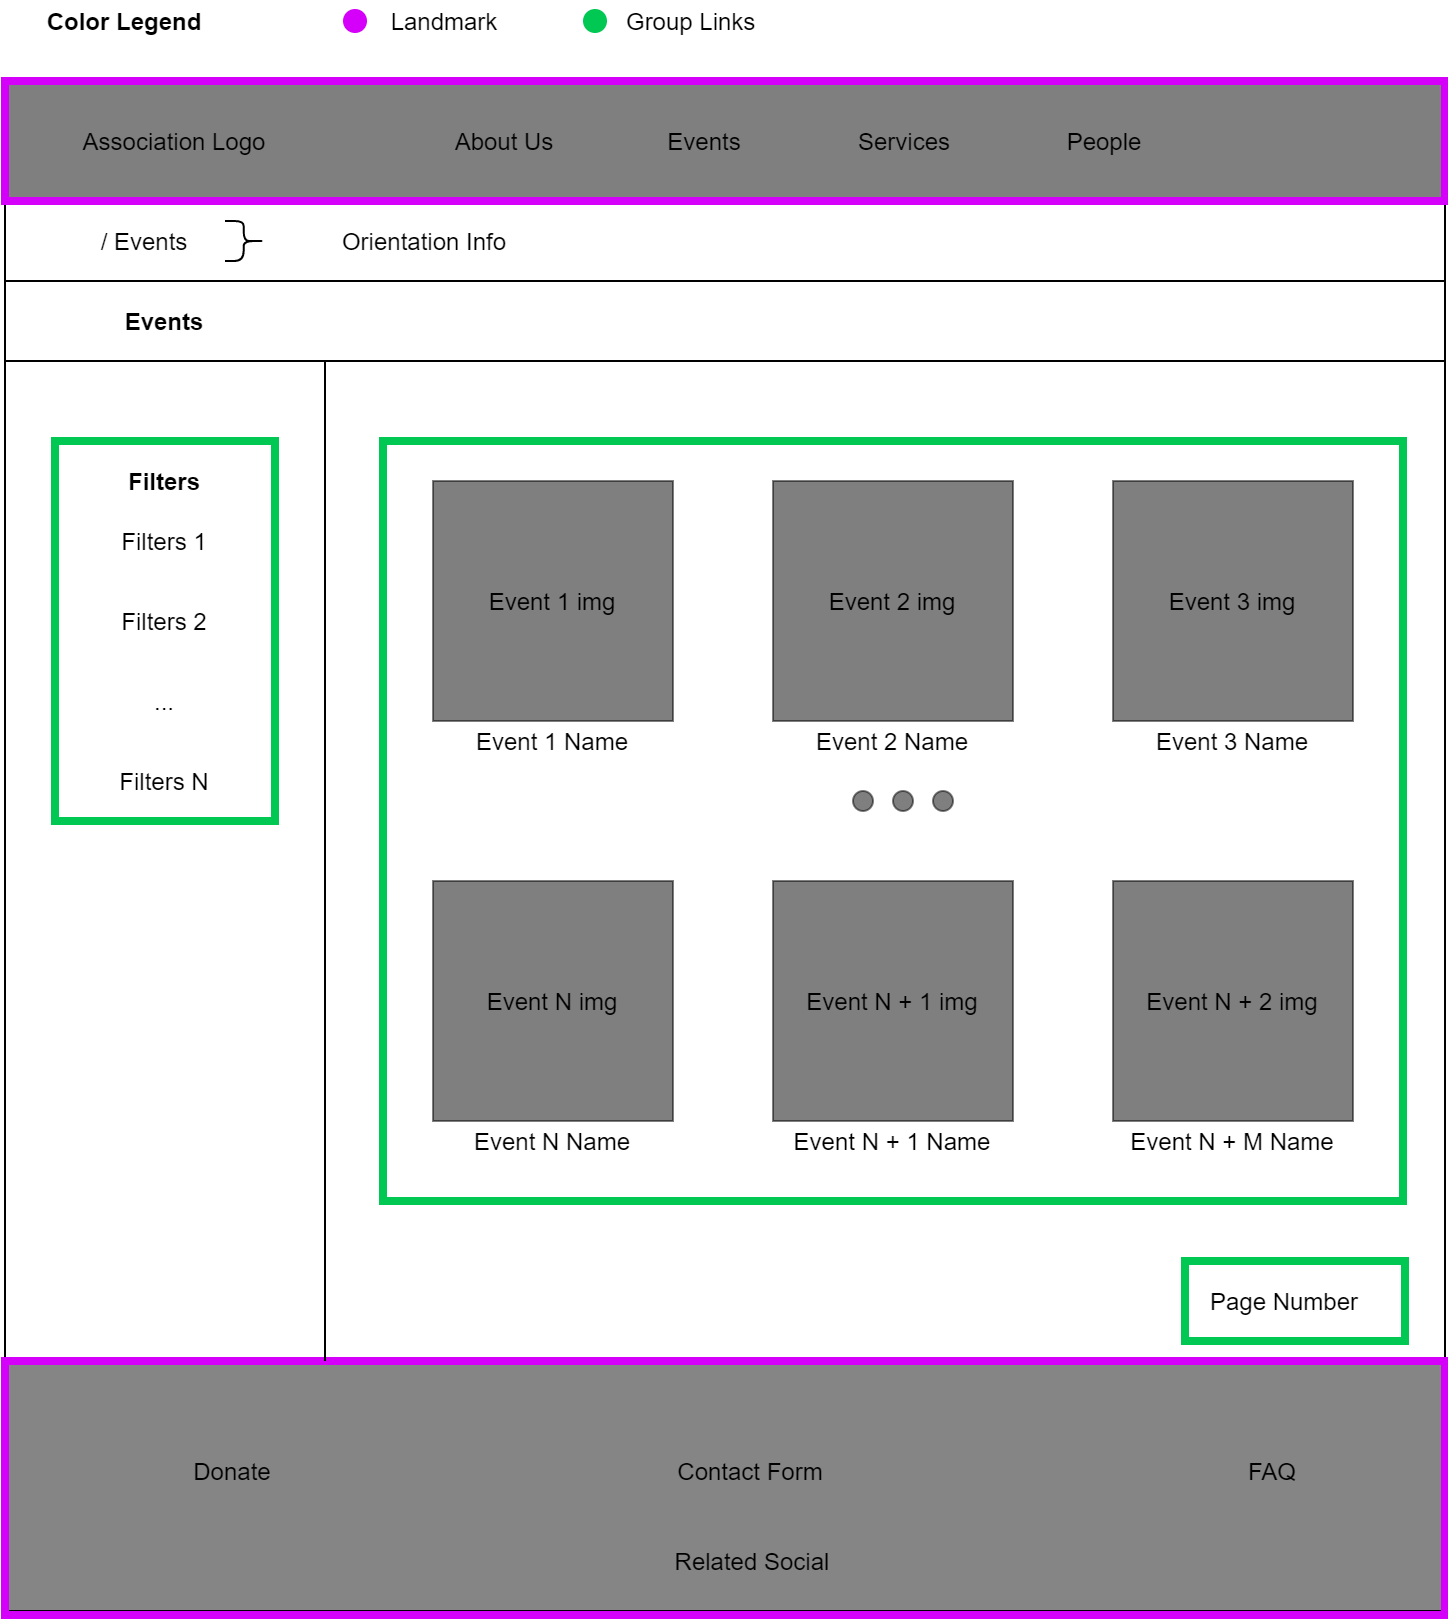
\includegraphics[width=\textwidth]{./assets/events.png}
			\caption{Events Page - Design in the small.}
		\end{minipage}
	\end{figure}
\FloatBarrier 

\clearpage

\subsubsection{Events screenshot}
\begin{figure}[h!]
	\centering
	\begin{minipage}[b]{1\textwidth}
    		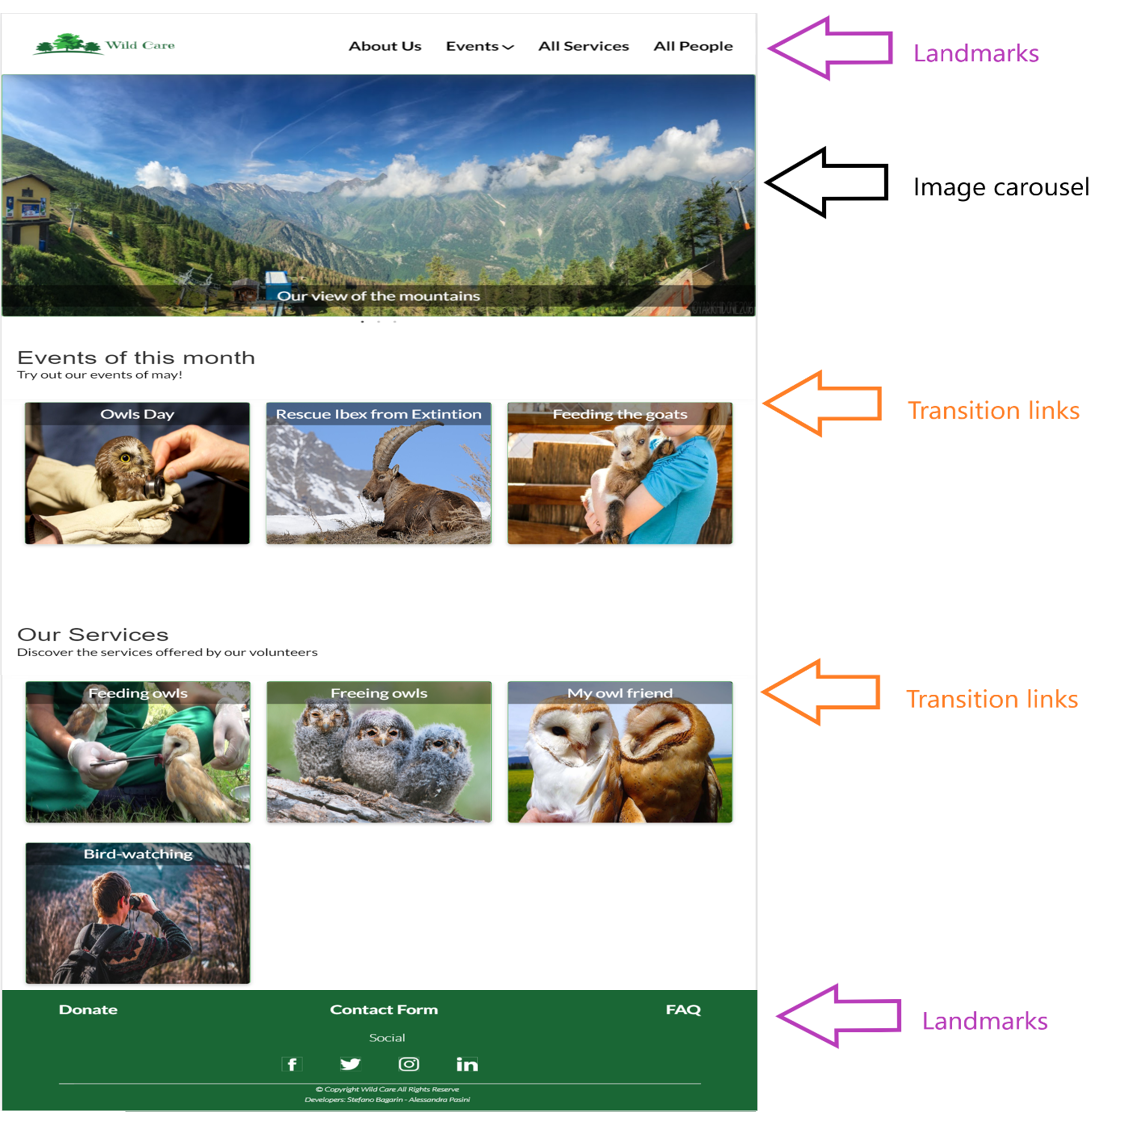
\includegraphics[width=\textwidth]{./assets/mockups/homepage_commented.png}
		\caption{Events Page - Screenshot commented.}
	\end{minipage}
\end{figure}
\FloatBarrier

\vspace{1cm}
\hspace{-1cm}
Events' details can be found in Event page, which contains:
\begin{itemize}
	\item all event's information stored into the database such as the promotion image, practical info (like event date and location),  			a brief description, etc. etc.
	\item the transition links to all services that the association provide during the selected event
	\item the transition link to the volunteers' details that are the point of reference and organizers of the selected event
\end{itemize} 

\clearpage

\subsubsection{Event in-the-small}
\begin{figure}[h!]
		\centering
		\begin{minipage}[b]{1\textwidth}
    			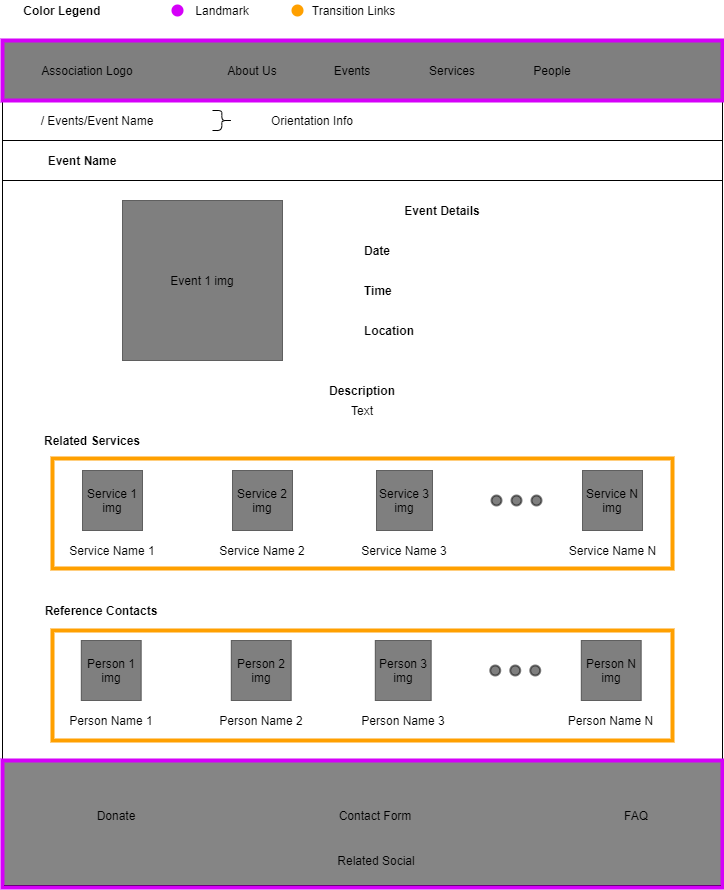
\includegraphics[width=\textwidth]{./assets/eventdetails.png}
			\caption{Event Page - Design in the small.}
		\end{minipage}
\end{figure}
\FloatBarrier

\clearpage

\subsubsection{Event screenshot}
\begin{figure}[h!]
	\centering
	\begin{minipage}[b]{1\textwidth}
    		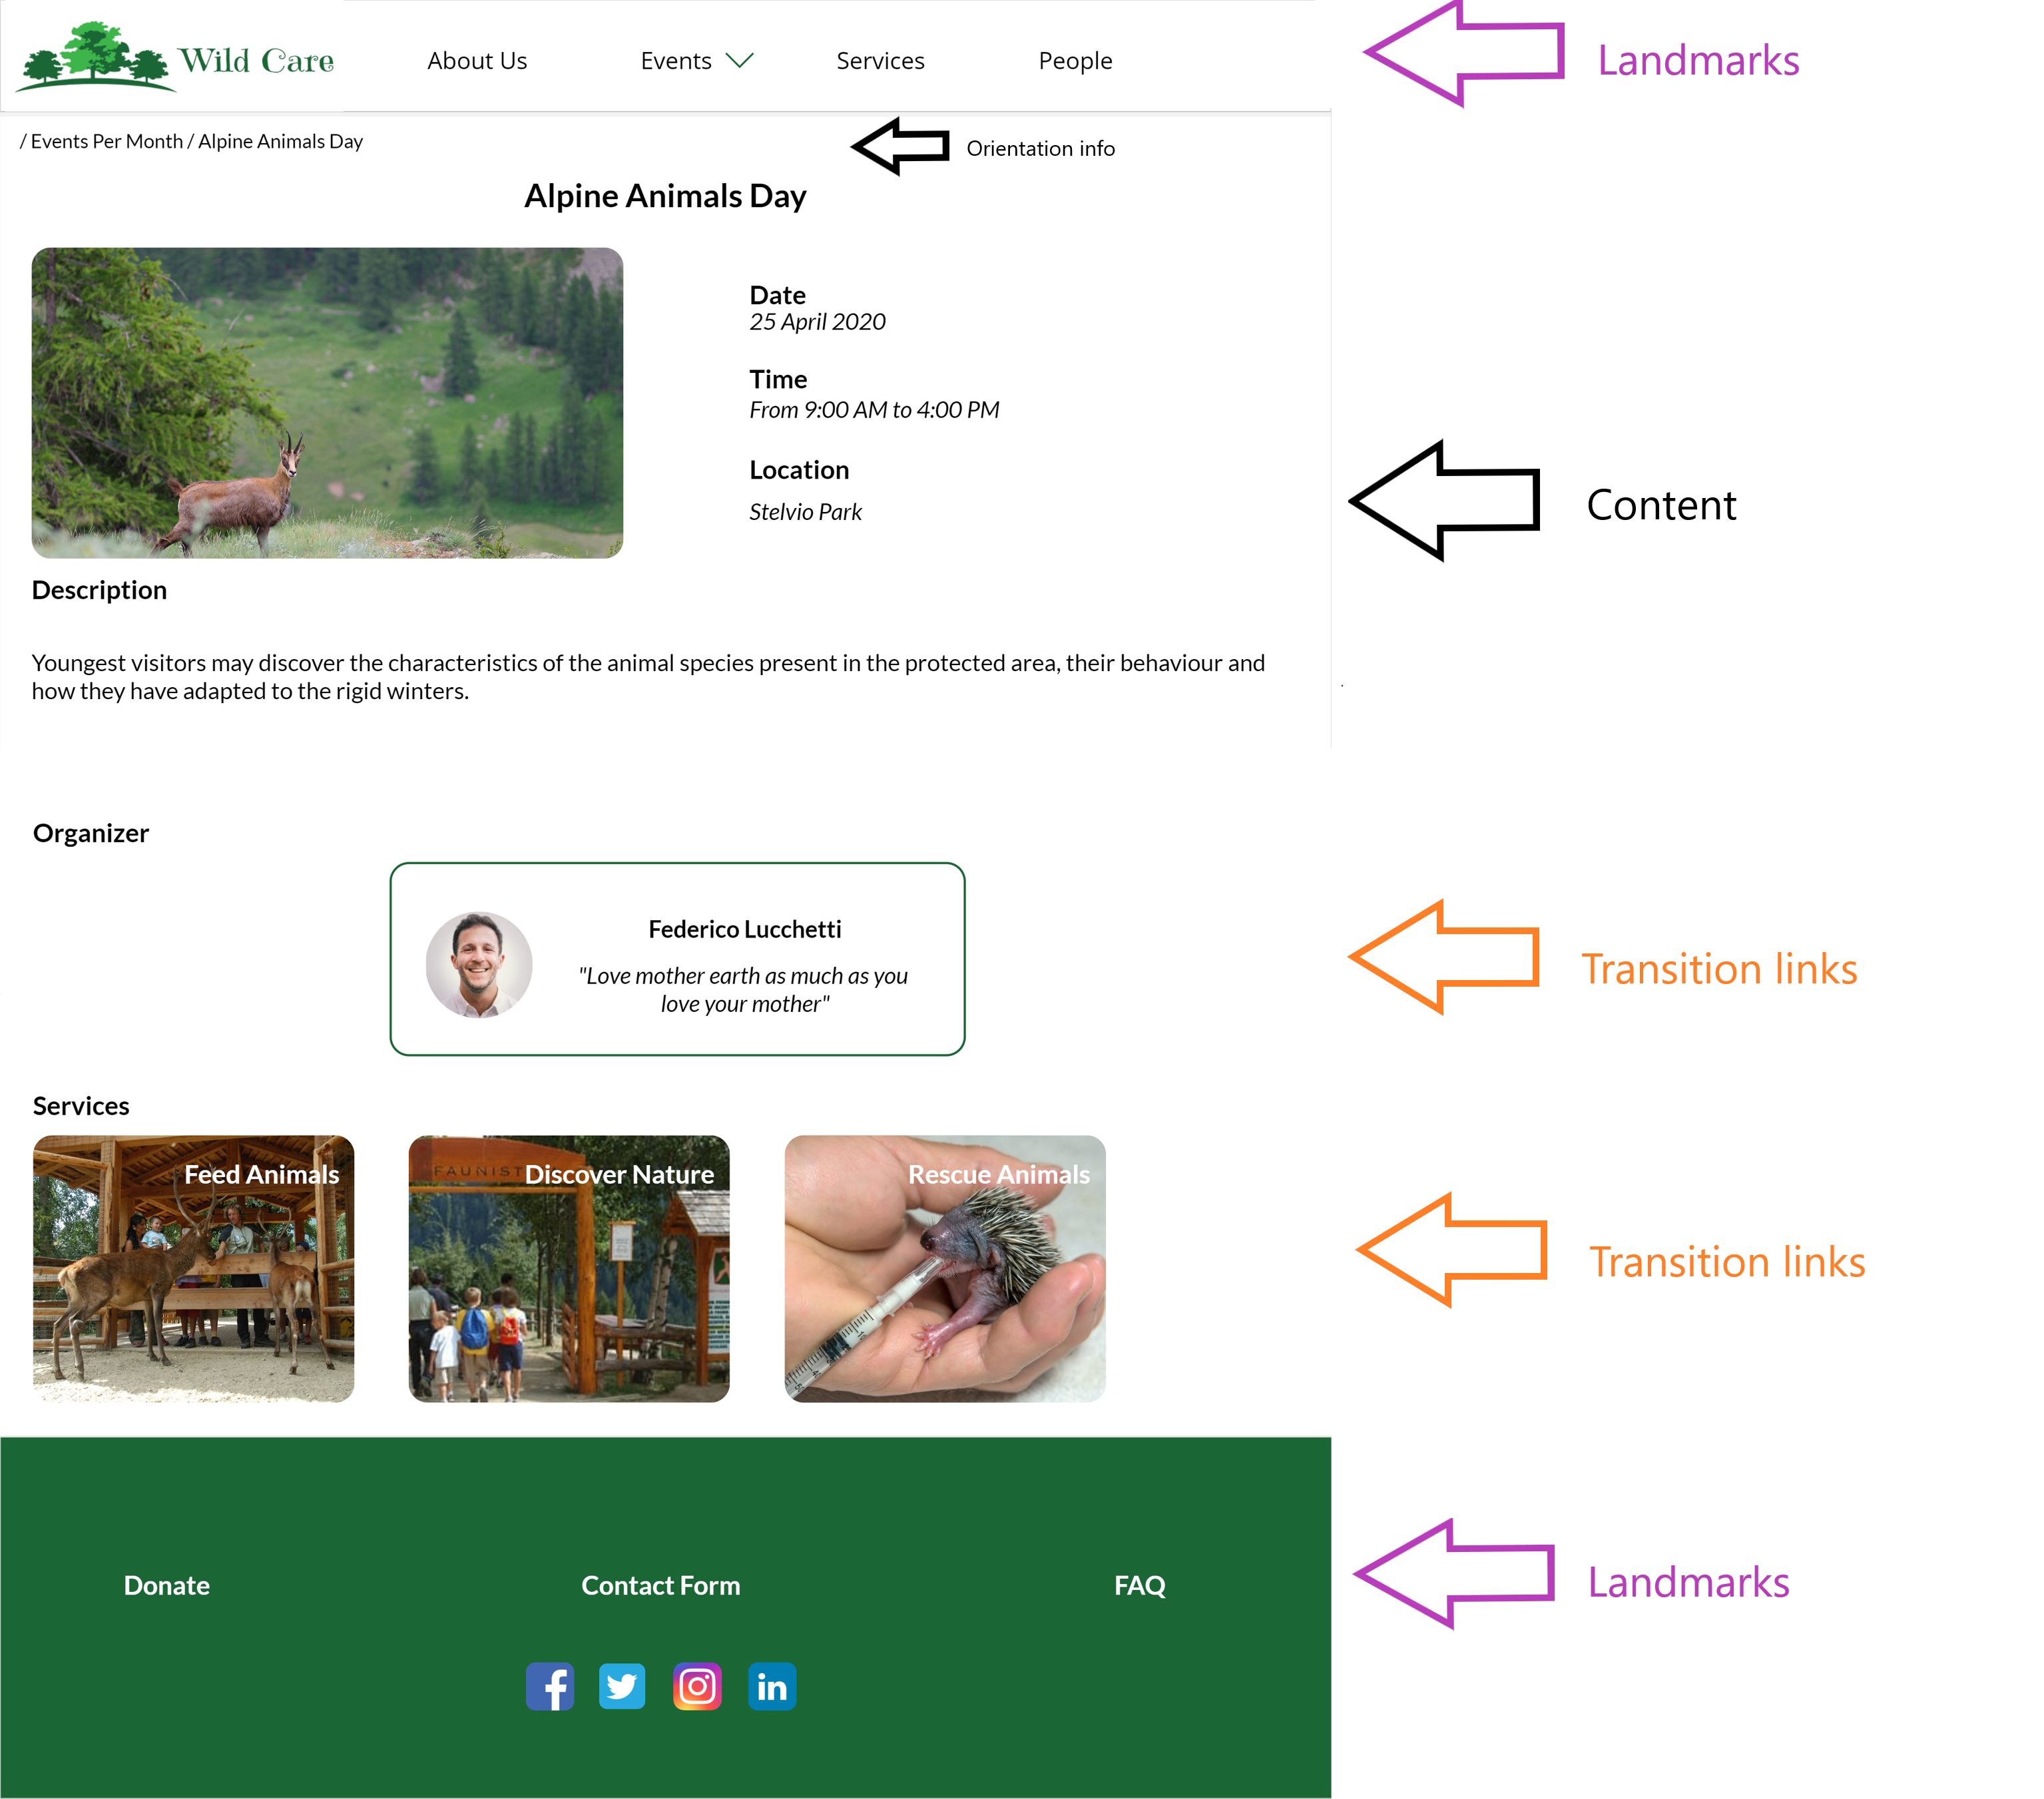
\includegraphics[width=\textwidth]{./assets/mockups/eventdetails_commented.png}
		\caption{Event Page - Screenshot commented.}
	\end{minipage}
\end{figure}
\FloatBarrier
	\clearpage

	\subsection{Services}
	The Services page aims to show all the services provided by our association. In the page is possible to click on each service image or name to access its dedicated page.

\begin{figure}[h!]
		\centering
		\begin{minipage}[b]{1\textwidth}
    			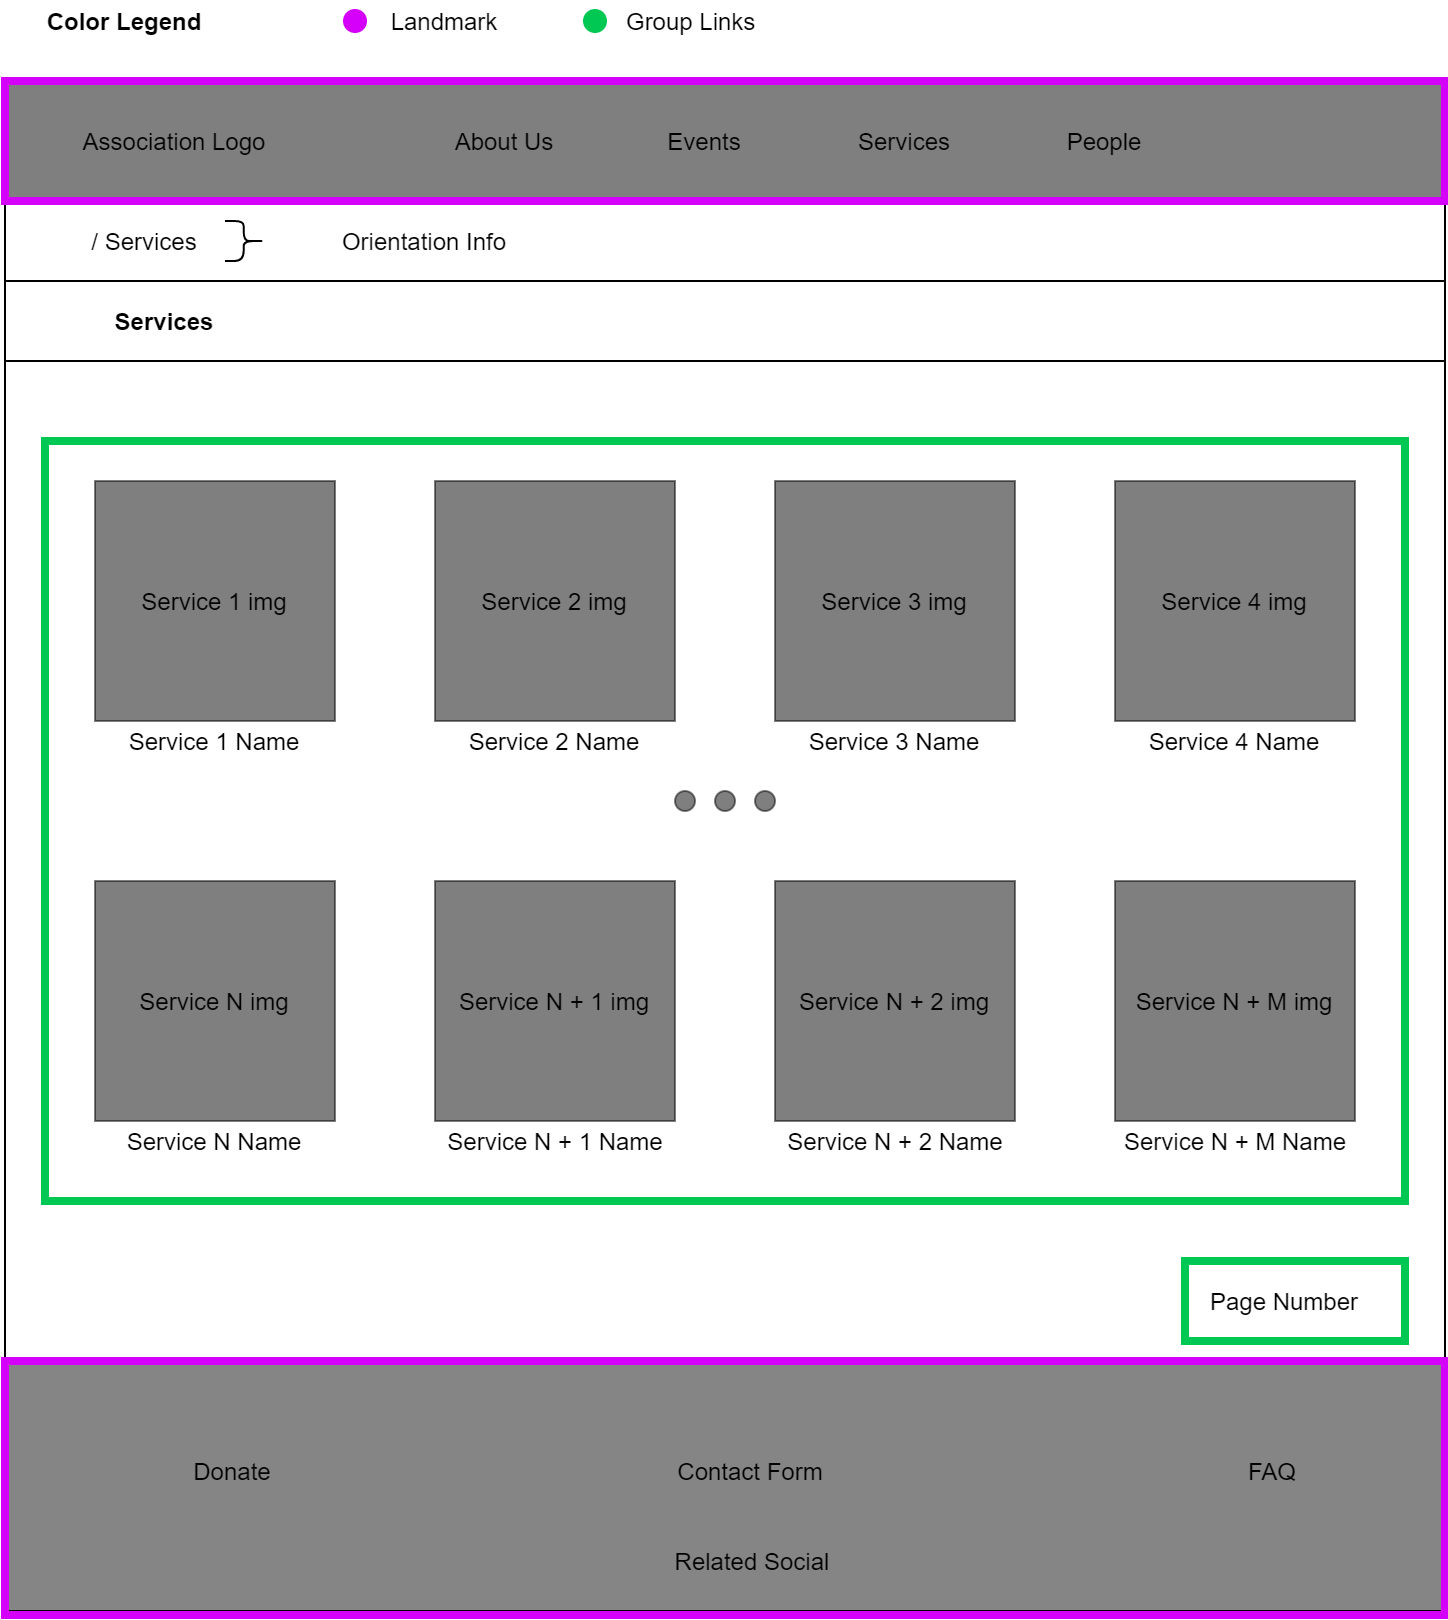
\includegraphics[width=\textwidth]{./assets/services.png}
			\caption{Services Page - Design in the small}
		\end{minipage}
	\end{figure}
\FloatBarrier
\vspace{1cm}
\hspace{-1cm}
Services' details can be found in Service page, which contains:
\begin{itemize}
	\item a carousel with all images related to the selected service, there must be at least one image and all of them are retrieved 			from the database;
	\item practical info and a brief description that explain the service purpose and all important information that users need;
	\item the transition links to the volunteer that are involved in the selected service;
	\item the transition links to the events in which the selected service is provided.
\end{itemize} 

\begin{figure}[h!]
		\centering
		\begin{minipage}[b]{1\textwidth}
    			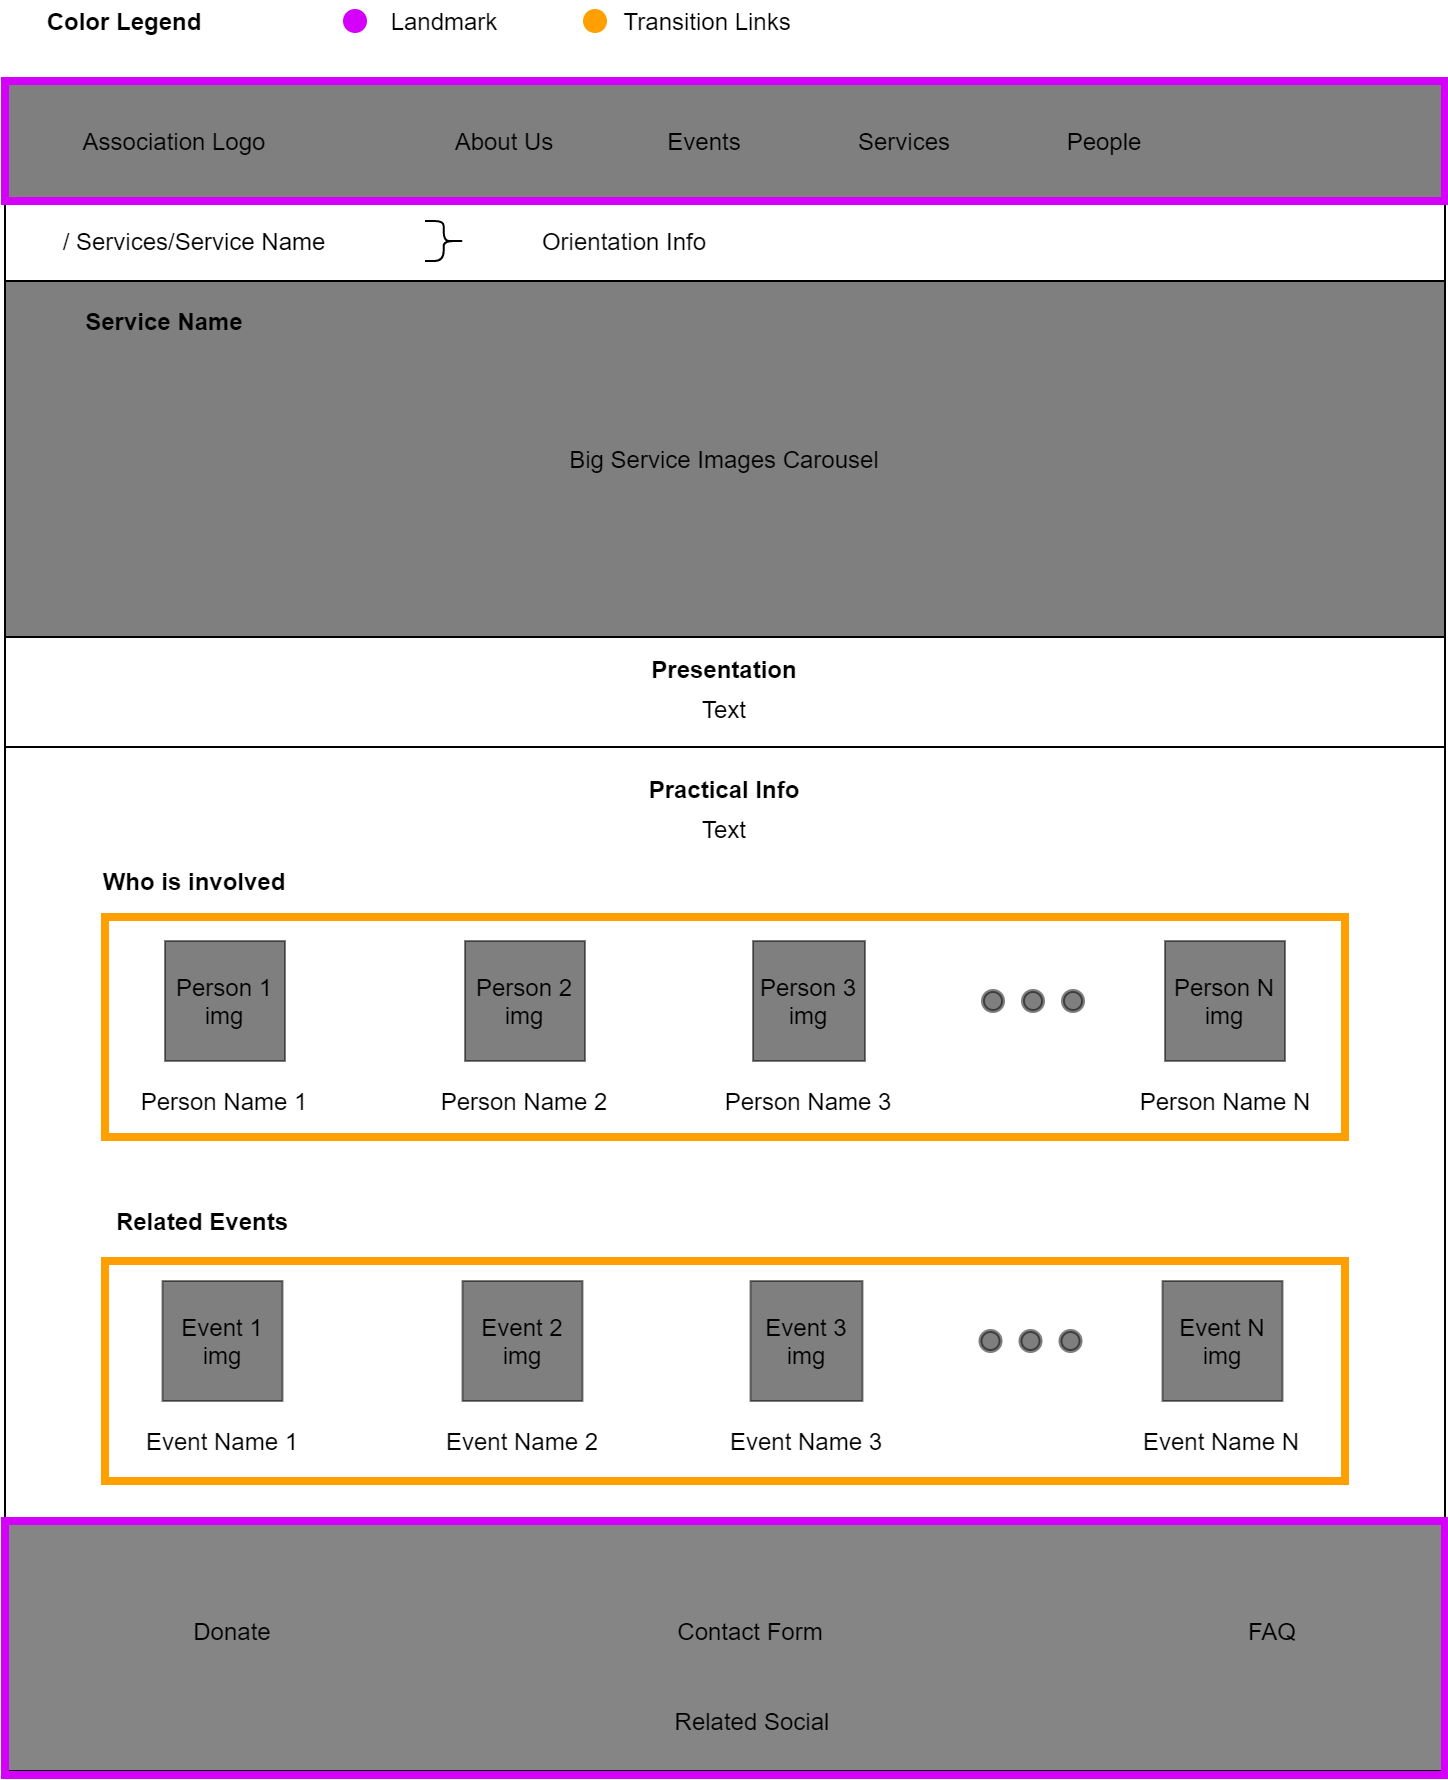
\includegraphics[width=\textwidth]{./assets/servicedetails.png}
			\caption{Service Page - Design in the small}
		\end{minipage}
\end{figure}
\FloatBarrier

	\clearpage

	\subsection{People}
	The \emph{People} page contains a grid with all volunteers that are part of our organization.  By clicking on each contact image or name, it is possible to navigate to the person's details page. It is possible to search a person by typing the name of the desired person  through the group links above the grid. 

\subsubsection{People in-the-small}
\begin{figure}[h!]
		\centering
		\begin{minipage}[b]{1\textwidth}
    			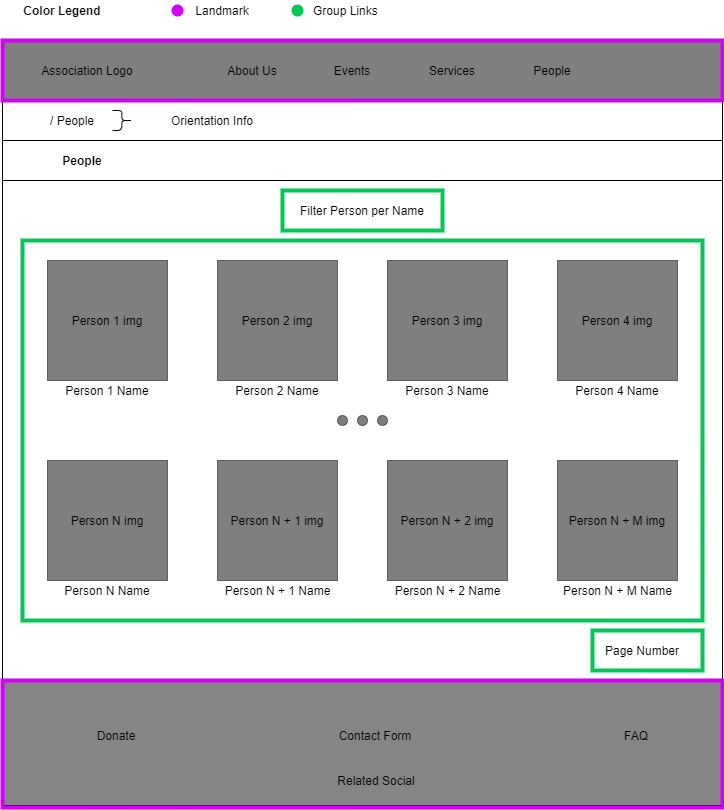
\includegraphics[width=\textwidth]{./assets/people.png}
			\caption{People Page - Design in the small.}
		\end{minipage}
	\end{figure}
	\FloatBarrier

\clearpage

\subsubsection{People screenshot}
\begin{figure}[h!]
	\centering
	\begin{minipage}[b]{1\textwidth}
    		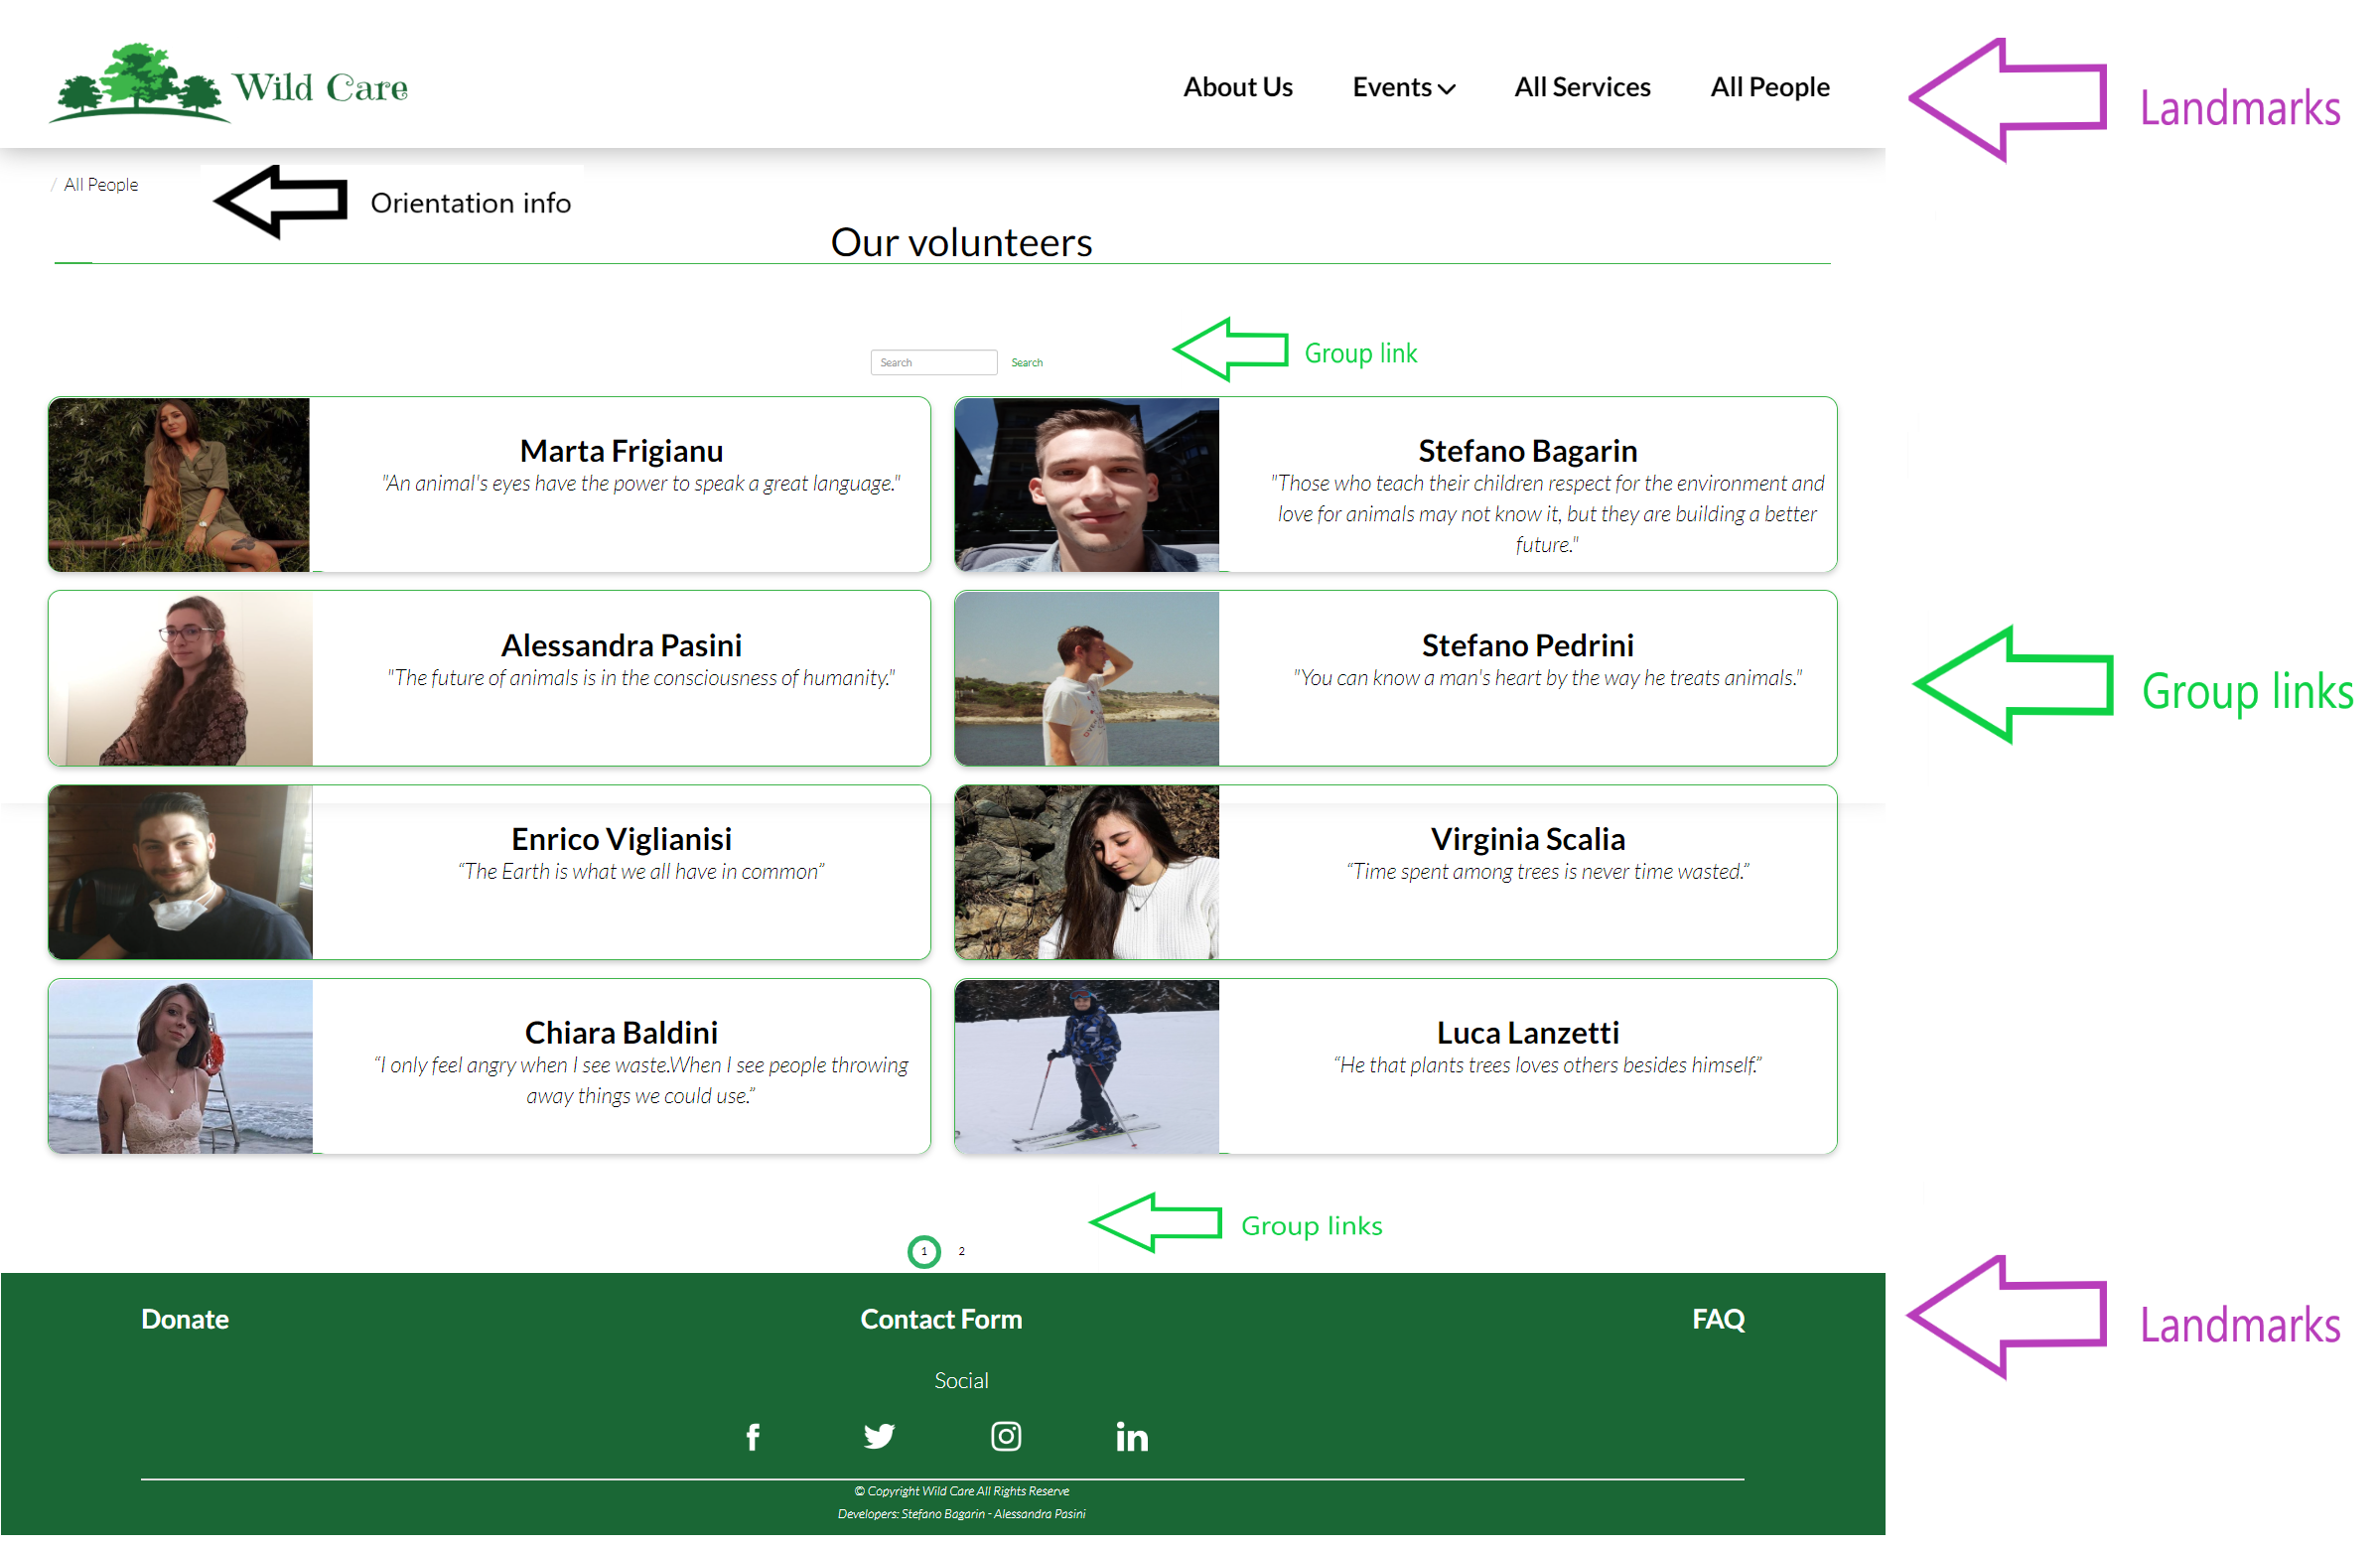
\includegraphics[width=\textwidth]{./assets/mockups/people_commented.png}
		\caption{People Page - Screenshot commented.}
	\end{minipage}
\end{figure}
\FloatBarrier

\vspace{1cm}
\hspace{-1cm}
People's details can be found in Person page, which contains:
\begin{itemize}
	\item all person's information stored into the database such as the contact image, anagraphics as name and birthday, contacts 			info as email and number,	a brief description, etc. etc.
	\item the transition links to all services the person is involved in
	\item the transition link to the events for which he/she is the point of reference. It may happen that a person doesn't have any 		transition link to events.
\end{itemize} 

\clearpage

\subsubsection{Person in-the-small}
\begin{figure}[h!]
		\centering
		\begin{minipage}[b]{1\textwidth}
    			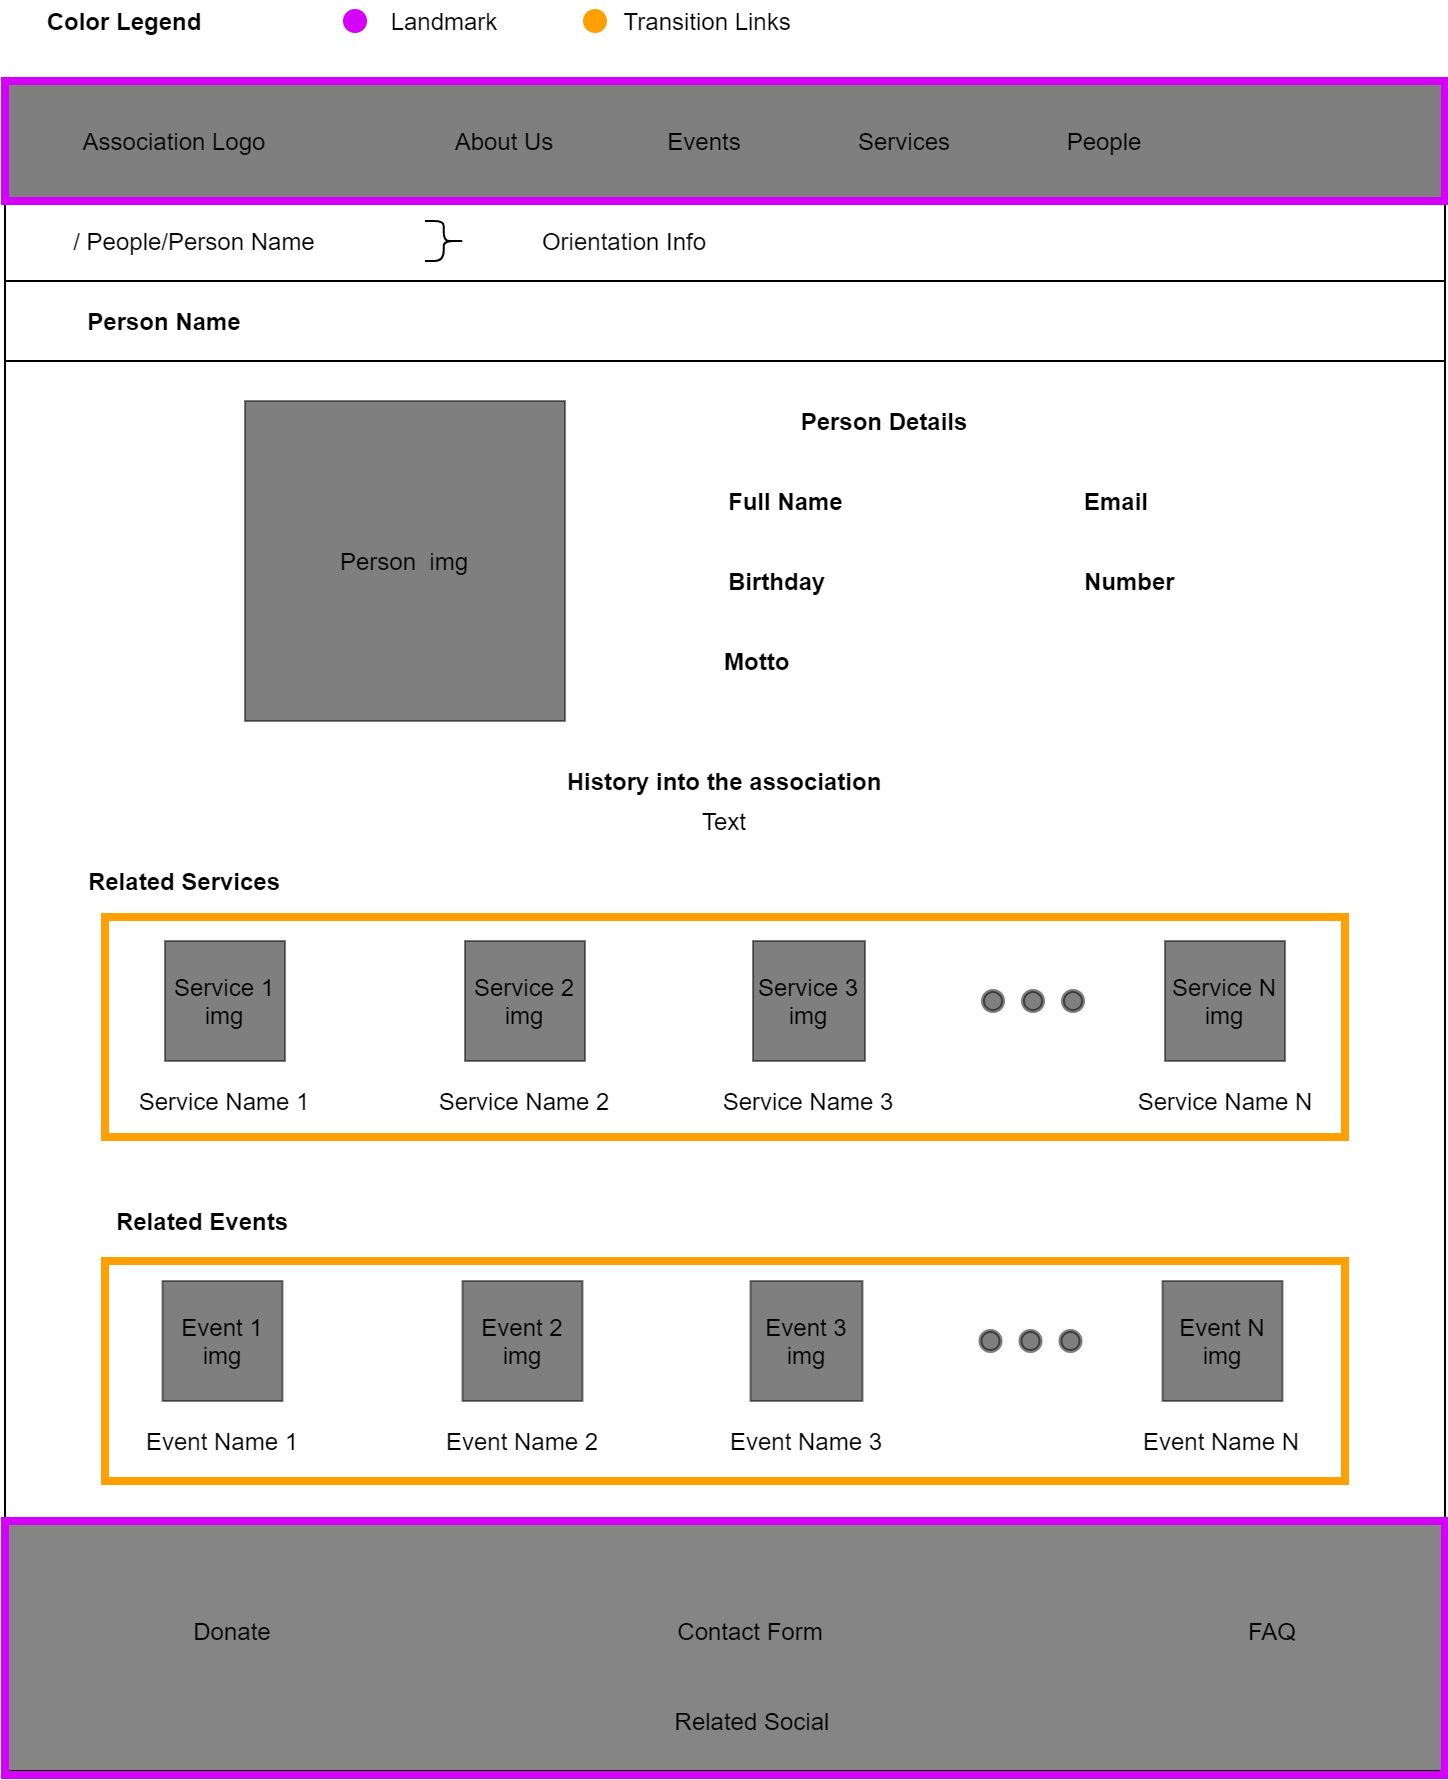
\includegraphics[width=\textwidth]{./assets/persondetails.png}
			\caption{Person Page - Design in the small.}
		\end{minipage}
\end{figure}
\FloatBarrier

\clearpage

\subsubsection{Person screenshot}
\begin{figure}[h!]
	\centering
	\begin{minipage}[b]{1\textwidth}
    		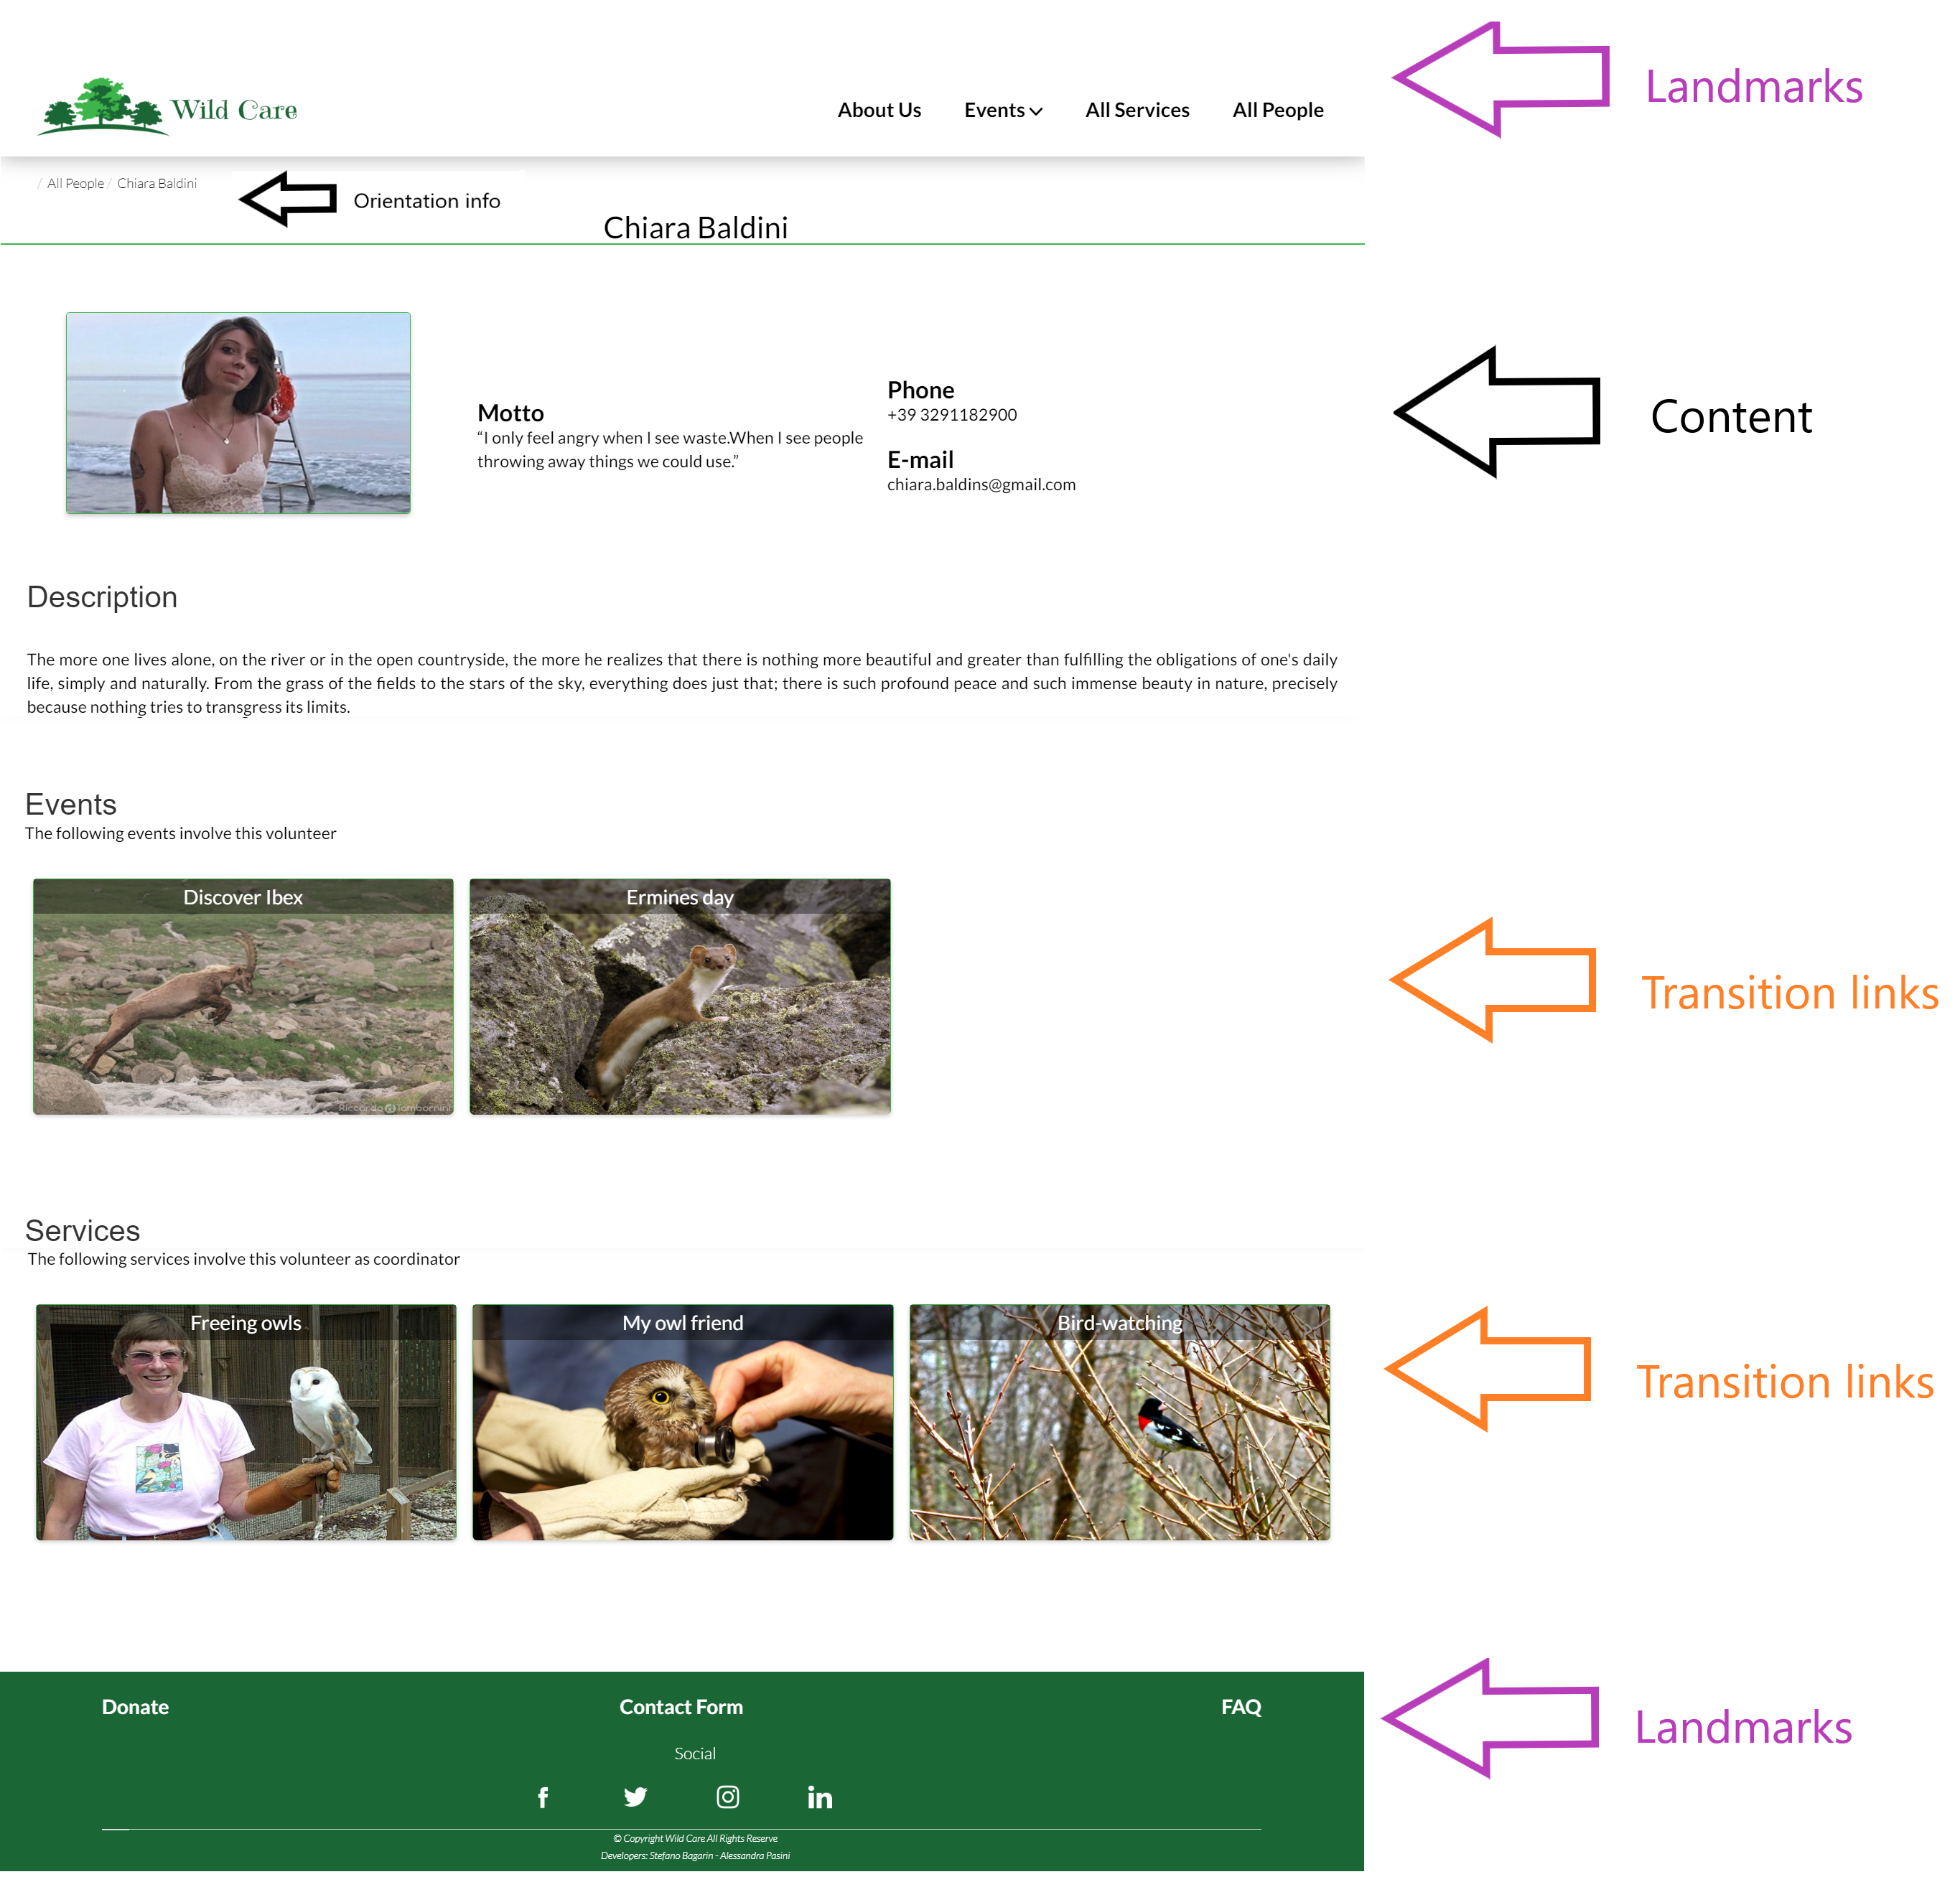
\includegraphics[width=\textwidth]{./assets/mockups/persondetails_commented.png}
		\caption{Person Page - Screenshot commented.}
	\end{minipage}
\end{figure}
\FloatBarrier

	\clearpage

	%Database Design
	\section{Database Design}	
	\subsection{Entity Relationship Diagram}
\begin{figure}[h!]
		\centering
		\begin{minipage}[b]{1\textwidth}
    			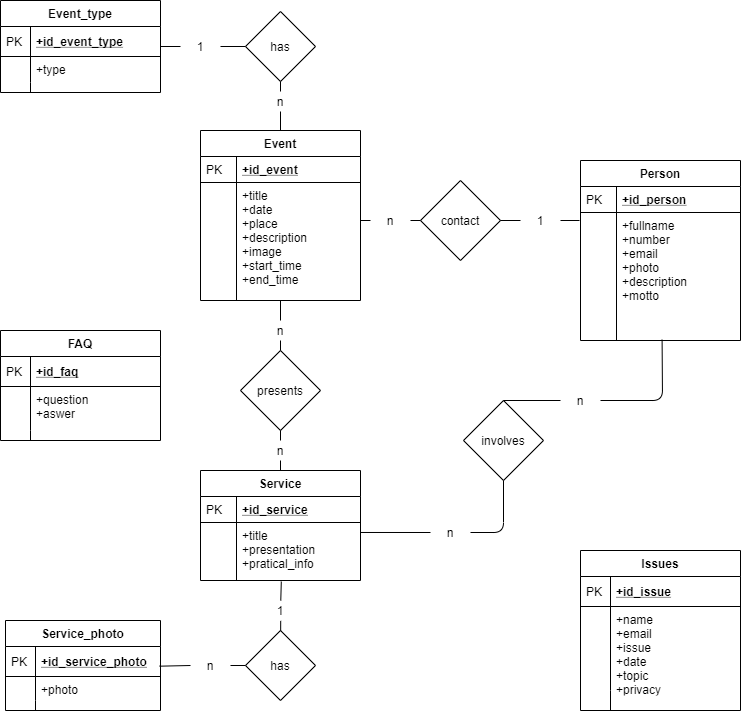
\includegraphics[width=\textwidth]{./assets/ER_diagram.png}
			\caption{Relationa database structure}
		\end{minipage}
\end{figure}
\FloatBarrier

\subsection{Logical Design}
\begin{figure}[h!]
		\centering
		\begin{minipage}[b]{1\textwidth}
    			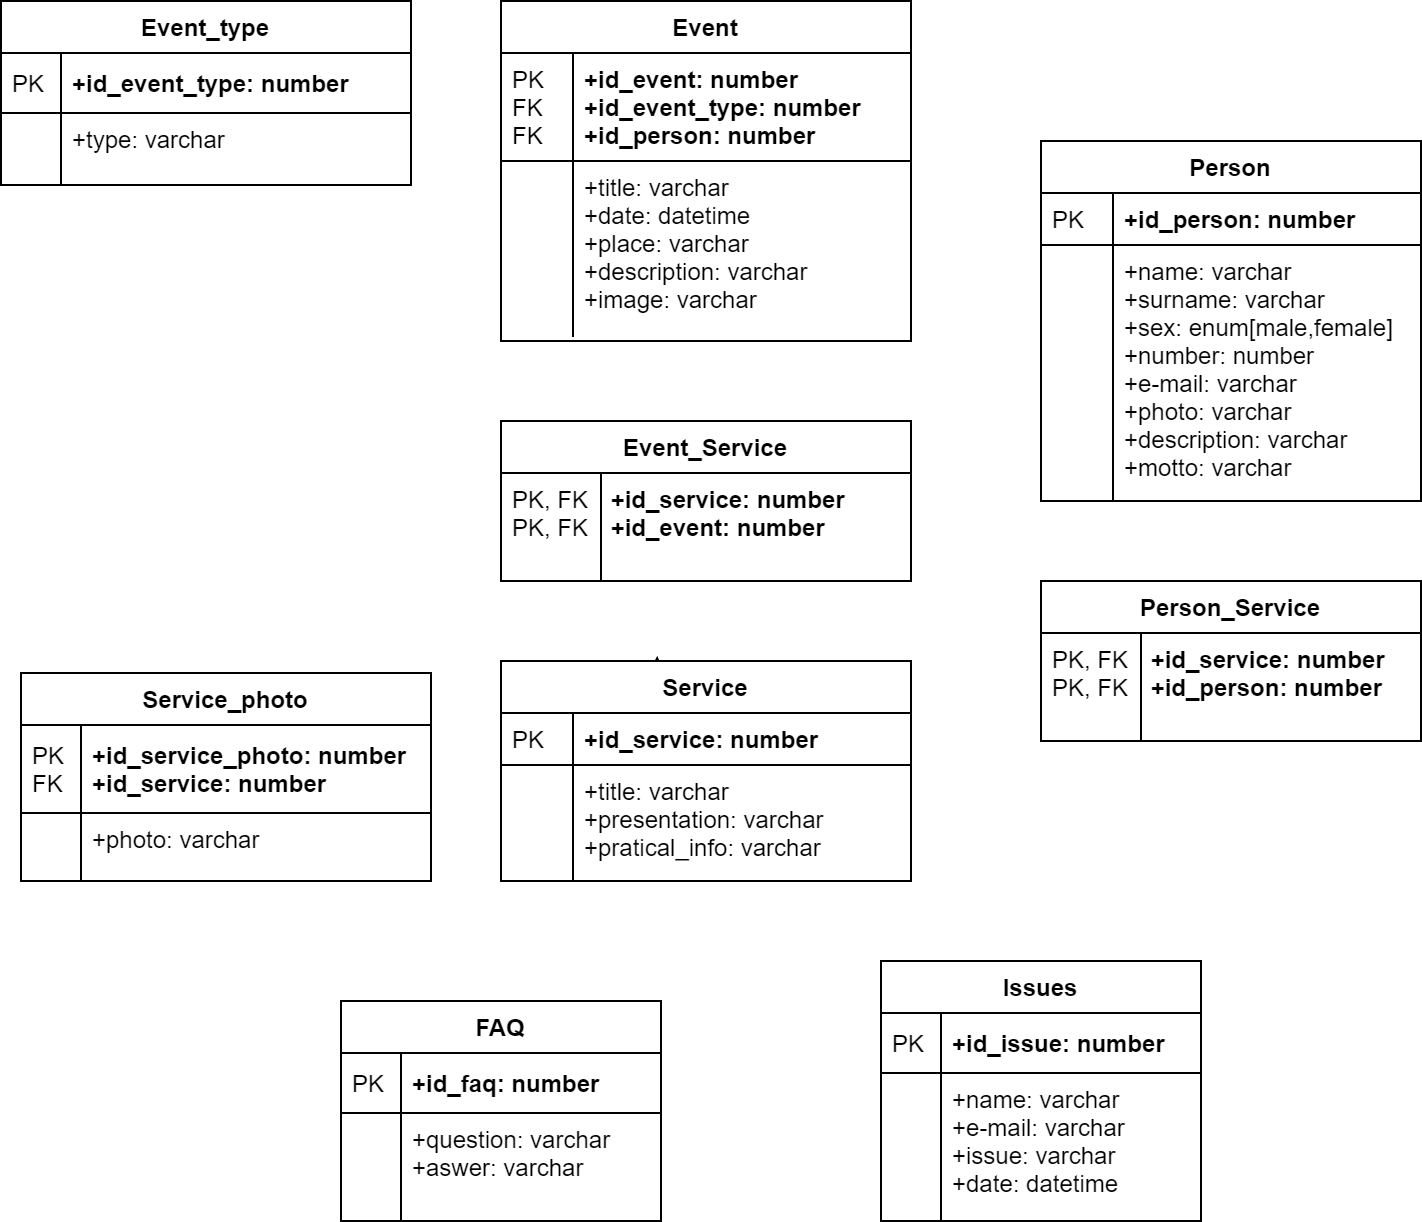
\includegraphics[width=\textwidth]{./assets/logical_diagram.png}
			\caption{Logic Diagram}
		\end{minipage}
\end{figure}
\FloatBarrier
	\clearpage

\end{document}
